%! TEX encoding = utf8
\chapter{Strojenie regulatorów}

\section{Strojenie regulatora PID}

Otrzymane metodą ZN nastawy regulatora PID: $K_p = 1.212$, $T_i = 25$, $T_d = 6$.

Wyniki symulacji o długości $n = 1000$ dla parametrów:

\begin{figure}[H]
\centering
% This file was created by matlab2tikz.
%
%The latest updates can be retrieved from
%  http://www.mathworks.com/matlabcentral/fileexchange/22022-matlab2tikz-matlab2tikz
%where you can also make suggestions and rate matlab2tikz.
%
\definecolor{mycolor1}{rgb}{0.00000,0.44700,0.74100}%
%
\begin{tikzpicture}

\begin{axis}[%
width=4.272in,
height=2.477in,
at={(0.717in,0.437in)},
scale only axis,
xmin=0,
xmax=1000,
xlabel style={font=\color{white!15!black}},
xlabel={k},
ymin=2.7,
ymax=3.3,
ylabel style={font=\color{white!15!black}},
ylabel={U(k)},
axis background/.style={fill=white}
]
\addplot[const plot, color=mycolor1, forget plot] table[row sep=crcr] {%
1	3\\
2	3\\
3	3\\
4	3\\
5	3\\
6	3\\
7	3\\
8	3\\
9	3\\
10	3\\
11	3\\
12	3.075\\
13	3\\
14	3.010908\\
15	3.021816\\
16	3.032724\\
17	3.043632\\
18	3.05454\\
19	3.065448\\
20	3.076356\\
21	3.087264\\
22	3.09191469752011\\
23	3.09741727832062\\
24	3.10835835125613\\
25	3.11750737390912\\
26	3.1250108978594\\
27	3.13100064174436\\
28	3.13559493994929\\
29	3.13890005313427\\
30	3.14101135355647\\
31	3.14201439694598\\
32	3.14250794272691\\
33	3.14294063245152\\
34	3.14278020245166\\
35	3.14177931378134\\
36	3.1402682170773\\
37	3.13852641489319\\
38	3.13678964332843\\
39	3.13525597785577\\
40	3.13409116673837\\
41	3.13343328373961\\
42	3.13335322632927\\
43	3.13383247556956\\
44	3.13486420669633\\
45	3.1365059224089\\
46	3.13880352112784\\
47	3.14175100658478\\
48	3.14530245748271\\
49	3.14938187331061\\
50	3.15389122280096\\
51	3.15871697571387\\
52	3.16373899268339\\
53	3.16884363447907\\
54	3.17392910744948\\
55	3.1788980143411\\
56	3.18365271580752\\
57	3.18810043023244\\
58	3.19216009684853\\
59	3.19576692078764\\
60	3.19887511824325\\
61	3.20145928463488\\
62	3.20351442574217\\
63	3.20505422526612\\
64	3.20610800785771\\
65	3.20671818134348\\
66	3.20693888887464\\
67	3.20683473364387\\
68	3.20647865252469\\
69	3.20594906024485\\
70	3.20532665313551\\
71	3.204691152359\\
72	3.20411820639786\\
73	3.2036766869687\\
74	3.20342658901048\\
75	3.20341754380349\\
76	3.20368775284877\\
77	3.2042632041204\\
78	3.2051572111113\\
79	3.20637037499849\\
80	3.20789102055502\\
81	3.20969609896609\\
82	3.21175251163974\\
83	3.21401877675729\\
84	3.21644693135622\\
85	3.21898455369573\\
86	3.22157681580101\\
87	3.22416851036904\\
88	3.22670600837553\\
89	3.22913909568702\\
90	3.23142262894762\\
91	3.23351795226113\\
92	3.23539402503051\\
93	3.23702822512007\\
94	3.23840680906491\\
95	3.23952503007343\\
96	3.24038693054133\\
97	3.24100483562034\\
98	3.24139857971575\\
99	3.24159450243768\\
100	3.2416242561606\\
101	3.24152347310586\\
102	3.2413303443867\\
103	3.24108416584193\\
104	3.24082390521021\\
105	3.24058684206487\\
106	3.24040732631155\\
107	3.24031569389836\\
108	3.24033737067748\\
109	3.24049218753209\\
110	3.24079392191255\\
111	3.24125007272064\\
112	3.24186186713928\\
113	3.24262448980073\\
114	3.24352751698417\\
115	3.24455553172707\\
116	3.24568889017145\\
117	3.24690460535588\\
118	3.2481773120481\\
119	3.24948027501448\\
120	3.25078640324349\\
121	3.25206923400092\\
122	3.25330385312492\\
123	3.25446772157392\\
124	3.25554138278464\\
125	3.25650903069557\\
126	3.25735892411485\\
127	3.25808363920763\\
128	3.25868015799453\\
129	3.25914979666205\\
130	3.25949798299406\\
131	3.25973389717417\\
132	3.25986999444394\\
133	3.25992143151442\\
134	3.2599054211295\\
135	3.25984054071331\\
136	3.25974602157868\\
137	3.25964104475028\\
138	3.25954406811984\\
139	3.25947220749259\\
140	3.25944069121739\\
141	3.25946240465201\\
142	3.25954753684479\\
143	3.25970333766841\\
144	3.25993398937761\\
145	3.26024059233535\\
146	3.26062126061046\\
147	3.26107131942994\\
148	3.26158359319132\\
149	3.26214877000154\\
150	3.26275582658519\\
151	3.18775582658519\\
152	3.26275582658519\\
153	3.25008041155606\\
154	3.23739527758428\\
155	3.22468807329857\\
156	3.21194754974633\\
157	3.19916391709557\\
158	3.18632913446267\\
159	3.17343712539862\\
160	3.16048391451837\\
161	3.15377810399708\\
162	3.14625809521469\\
163	3.13348055632454\\
164	3.12280047384998\\
165	3.11404825287222\\
166	3.10707344616727\\
167	3.10174270549796\\
168	3.09793787409405\\
169	3.09555421773024\\
170	3.09449879311874\\
171	3.09416247028182\\
172	3.09407943116812\\
173	3.09475080182685\\
174	3.09637395368134\\
175	3.09856511377248\\
176	3.10099918347829\\
177	3.10340136815166\\
178	3.10553990613315\\
179	3.1072197719981\\
180	3.10827724100355\\
181	3.1086191373126\\
182	3.10824555763141\\
183	3.10715010913705\\
184	3.1052694919129\\
185	3.10256058393729\\
186	3.09903964002374\\
187	3.09476854432025\\
188	3.08984355124333\\
189	3.08438612116808\\
190	3.07853551256148\\
191	3.07243917595955\\
192	3.06623897062675\\
193	3.06006505214241\\
194	3.0540423275578\\
195	3.0482939102857\\
196	3.04293493202231\\
197	3.03806491131289\\
198	3.03376275590333\\
199	3.03008380003981\\
200	3.02705839039121\\
201	3.024691933976\\
202	3.0229668082165\\
203	3.02184567058965\\
204	3.02127440295111\\
205	3.02118398469599\\
206	3.02149242843138\\
207	3.02210765743975\\
208	3.02293114543814\\
209	3.02386188364982\\
210	3.02480036480803\\
211	3.02565234519747\\
212	3.02633213883109\\
213	3.02676522460351\\
214	3.02689014813192\\
215	3.02665989847518\\
216	3.02604288512225\\
217	3.02502346671072\\
218	3.02360193182578\\
219	3.0217938900634\\
220	3.01962909424838\\
221	3.01714975642257\\
222	3.01440845351454\\
223	3.01146574760512\\
224	3.00838765362728\\
225	3.00524306241698\\
226	3.00210119328099\\
227	2.99902913827057\\
228	2.99608956746295\\
229	2.99333867039806\\
230	2.99082440450804\\
231	2.98858510911683\\
232	2.9866485263773\\
233	2.98503124976018\\
234	2.9837385987712\\
235	2.98276489991566\\
236	2.98209414157647\\
237	2.98170096275648\\
238	2.98155192884752\\
239	2.98160704023913\\
240	2.9818214126496\\
241	2.98214706296971\\
242	2.98253473203313\\
243	2.98293567652367\\
244	2.98330336631223\\
245	2.98359503043995\\
246	2.9837730037168\\
247	2.9838058354662\\
248	2.9836691318205\\
249	2.9833461131237\\
250	2.98282787843086\\
251	2.98211337961419\\
252	2.98120911783444\\
253	2.98012858467236\\
254	2.97889147859116\\
255	2.97752273422936\\
256	2.97605140707064\\
257	2.97450945924595\\
258	2.97293049366354\\
259	2.97134848343638\\
260	2.96979654177645\\
261	2.9683057742507\\
262	2.96690425067718\\
263	2.96561612816678\\
264	2.96446095012603\\
265	2.9634531387154\\
266	2.96260169061596\\
267	2.96191007830416\\
268	2.9613763516488\\
269	2.96099342777139\\
270	2.96074955095883\\
271	2.96062889916217\\
272	2.96061230940251\\
273	2.96067809134281\\
274	2.96080289643911\\
275	2.96096260947722\\
276	2.96113322990344\\
277	2.96129171209649\\
278	2.96141673649013\\
279	2.96148938709612\\
280	2.96149371532908\\
281	2.96141717491345\\
282	2.96125091786529\\
283	2.96098994689099\\
284	2.96063312483552\\
285	2.96018304686046\\
286	2.95964578566525\\
287	2.95903052413774\\
288	2.95834909320886\\
289	2.95761543530168\\
290	2.9568450155458\\
291	2.95605420384761\\
292	2.95525965096874\\
293	2.95447768100315\\
294	2.9537237211191\\
295	2.9530117872315\\
296	2.95235404149999\\
297	2.95176043432946\\
298	2.95123844001745\\
299	2.95079289148438\\
300	2.95042591577759\\
301	3.02542591577759\\
302	2.95042591577759\\
303	2.95512942908458\\
304	2.95989499919844\\
305	2.96471346489173\\
306	2.96957436038736\\
307	2.97446633800435\\
308	2.97937760437466\\
309	2.98429635417871\\
310	2.98921118611112\\
311	2.98783007750046\\
312	2.98723815650551\\
313	2.99254644075\\
314	2.99697245873784\\
315	3.00058131129338\\
316	3.0034329483037\\
317	3.00558286939169\\
318	3.00708269150639\\
319	3.00798059424612\\
320	3.00832165520727\\
321	3.00867215125167\\
322	3.00945645971642\\
323	3.01007893769673\\
324	3.01015599987653\\
325	3.00986482751503\\
326	3.00935714308678\\
327	3.00876235951009\\
328	3.00819032895181\\
329	3.00773374925175\\
330	3.00747027883543\\
331	3.00742068136657\\
332	3.00752432641724\\
333	3.00774217487303\\
334	3.00811769827039\\
335	3.00870656015214\\
336	3.00953357578893\\
337	3.01059919377235\\
338	3.01188491978975\\
339	3.01335783957974\\
340	3.01497437478075\\
341	3.0166870331934\\
342	3.01845593571681\\
343	3.02025273517867\\
344	3.02205101974527\\
345	3.02381857986731\\
346	3.02551944876457\\
347	3.02711862163017\\
348	3.0285854193973\\
349	3.02989577412236\\
350	3.03103366466919\\
351	3.03199158656542\\
352	3.03276950256207\\
353	3.03337265675386\\
354	3.03381007126073\\
355	3.03409457691489\\
356	3.03424328769332\\
357	3.03427748809872\\
358	3.03422188393634\\
359	3.03410346517824\\
360	3.0339501673144\\
361	3.03378949337594\\
362	3.0336473005721\\
363	3.03354695047589\\
364	3.03350882373911\\
365	3.03354998629113\\
366	3.03368383577379\\
367	3.03391974322731\\
368	3.03426278924895\\
369	3.03471366890098\\
370	3.03526879856596\\
371	3.0359206272797\\
372	3.0366581253909\\
373	3.0374673932672\\
374	3.03833232196624\\
375	3.03923526125113\\
376	3.04015768515945\\
377	3.04108085840625\\
378	3.04198649716753\\
379	3.04285740429348\\
380	3.0436780519899\\
381	3.04443508433414\\
382	3.045117716226\\
383	3.04571801407145\\
384	3.04623105472377\\
385	3.04665496838597\\
386	3.04699087484521\\
387	3.04724272194818\\
388	3.04741703459842\\
389	3.04752258388925\\
390	3.04756998887373\\
391	3.04757126675004\\
392	3.04753934997139\\
393	3.04748759026387\\
394	3.04742926929756\\
395	3.04737713391996\\
396	3.04734297117707\\
397	3.04733723566256\\
398	3.0473687393843\\
399	3.04744441213782\\
400	3.04756913802734\\
401	3.0477456711302\\
402	3.04797463039486\\
403	3.04825457086069\\
404	3.04858212543498\\
405	3.0489522090097\\
406	3.0493582748072\\
407	3.04979261152713\\
408	3.0502466690488\\
409	3.05071140004138\\
410	3.05117760481453\\
411	3.05163626710853\\
412	3.05207886928934\\
413	3.05249767657633\\
414	3.05288598145428\\
415	3.05323830123165\\
416	3.05355052370736\\
417	3.05381999799186\\
418	3.05404556960575\\
419	3.05422756097972\\
420	3.05436770034909\\
421	3.05446900372524\\
422	3.05453561609009\\
423	3.05457261915414\\
424	3.05458581390707\\
425	3.05458148674669\\
426	3.05456616818777\\
427	3.05454639303323\\
428	3.05452847045843\\
429	3.05451827174703\\
430	3.05452104246284\\
431	3.05454124469118\\
432	3.05458243368165\\
433	3.0546471718239\\
434	3.0547369814406\\
435	3.05485233644112\\
436	3.05499269149694\\
437	3.05515654612345\\
438	3.05534153992342\\
439	3.05554457429986\\
440	3.05576195520501\\
441	3.05598955097505\\
442	3.05622295901606\\
443	3.05645767505453\\
444	3.05668925883931\\
445	3.05691349056465\\
446	3.0571265128544\\
447	3.05732495387699\\
448	3.05750602801744\\
449	3.05766761147949\\
450	3.05780829119128\\
451	3.05792738640409\\
452	3.05802494336783\\
453	3.05810170440643\\
454	3.0581590535687\\
455	3.0581989417701\\
456	3.05822379494568\\
457	3.0582364091894\\
458	3.05823983714929\\
459	3.05823727007856\\
460	3.05823191991154\\
461	3.05822690554843\\
462	3.05822514720747\\
463	3.05822927225404\\
464	3.05824153536584\\
465	3.05826375526372\\
466	3.05829726955641\\
467	3.0583429085391\\
468	3.05840098807814\\
469	3.05847132103091\\
470	3.05855324601575\\
471	3.05864567178067\\
472	3.05874713494004\\
473	3.05885586846791\\
474	3.05896987806477\\
475	3.05908702335669\\
476	3.05920510084231\\
477	3.05932192557088\\
478	3.05943540870673\\
479	3.05954362840123\\
480	3.05964489173938\\
481	3.05973778593886\\
482	3.05982121743766\\
483	3.0598944379933\\
484	3.05995705741474\\
485	3.06000904303835\\
486	3.06005070652486\\
487	3.06008267897993\\
488	3.06010587577328\\
489	3.06012145273854\\
490	3.06013075567153\\
491	3.06013526520137\\
492	3.0601365391858\\
493	3.06013615477941\\
494	3.0601356522444\\
495	3.06013648242495\\
496	3.06013995959468\\
497	3.06014722112486\\
498	3.0601591951173\\
499	3.06017657681548\\
500	3.06019981426158\\
501	3.13519981426158\\
502	3.06019981426158\\
503	3.06145281489043\\
504	3.06271102562167\\
505	3.06397375714421\\
506	3.06524016564909\\
507	3.06650928973373\\
508	3.0677800899163\\
509	3.06905148924817\\
510	3.07032241353731\\
511	3.06533697089846\\
512	3.06120600206443\\
513	3.06332133103454\\
514	3.06514756309781\\
515	3.06670883872709\\
516	3.06802701345722\\
517	3.06912190169898\\
518	3.07001149167258\\
519	3.07071213379151\\
520	3.07123870484846\\
521	3.0721265976191\\
522	3.07376745605835\\
523	3.07551068804718\\
524	3.07687998815798\\
525	3.07795172960008\\
526	3.07879172736933\\
527	3.07945657273642\\
528	3.07999480544429\\
529	3.08044794327634\\
530	3.08085138645092\\
531	3.08119167421284\\
532	3.08138146495911\\
533	3.08136384872773\\
534	3.08117740274781\\
535	3.08088843685575\\
536	3.08054606989055\\
537	3.08018534561367\\
538	3.07982986338876\\
539	3.07949399284336\\
540	3.07918473233858\\
541	3.07890689529885\\
542	3.07867332010569\\
543	3.07850751278987\\
544	3.07843242947433\\
545	3.07846071307021\\
546	3.07859482002796\\
547	3.07883040396058\\
548	3.07915894073597\\
549	3.0795697354732\\
550	3.08005142874698\\
551	3.15505142874698\\
552	3.08005142874698\\
553	3.08188739573397\\
554	3.08374182225916\\
555	3.08559715505738\\
556	3.08743612502307\\
557	3.08924306556534\\
558	3.09100463777861\\
559	3.09271012447919\\
560	3.09435142008839\\
561	3.08971070436468\\
562	3.08593673724441\\
563	3.08837132731893\\
564	3.09043472383046\\
565	3.09215663880269\\
566	3.09356662301866\\
567	3.09469396703591\\
568	3.09556744663615\\
569	3.09621500787634\\
570	3.09666345551231\\
571	3.09745646575836\\
572	3.09898709353326\\
573	3.10060720921155\\
574	3.10185040331946\\
575	3.10280516342765\\
576	3.10354735634633\\
577	3.10414143496713\\
578	3.10464155607561\\
579	3.1050926354\\
580	3.10553135109211\\
581	3.10594385695111\\
582	3.10624176138622\\
583	3.10636694787428\\
584	3.10635593821051\\
585	3.10627143348261\\
586	3.10615751073673\\
587	3.10604319515026\\
588	3.10594552192289\\
589	3.10587214746192\\
590	3.10582356079234\\
591	3.10579854782488\\
592	3.10580453745707\\
593	3.10586024896688\\
594	3.10598449749623\\
595	3.10618656635026\\
596	3.10646650491181\\
597	3.10681862321267\\
598	3.10723414854235\\
599	3.10770319607028\\
600	3.10821618275658\\
601	3.18321618275658\\
602	3.10821618275658\\
603	3.11002077583757\\
604	3.11183077343174\\
605	3.11363306338932\\
606	3.11541490744774\\
607	3.11716509570219\\
608	3.11887451004634\\
609	3.12053627011361\\
610	3.12214559733615\\
611	3.11748797018653\\
612	3.1137129363882\\
613	3.11616320963362\\
614	3.11826085122342\\
615	3.12003545696909\\
616	3.12151578090694\\
617	3.12272969068594\\
618	3.12370398822883\\
619	3.12446418791554\\
620	3.12503431178895\\
621	3.12595496936073\\
622	3.12761609498234\\
623	3.12936657202842\\
624	3.13073703639327\\
625	3.13181313492648\\
626	3.13266820214814\\
627	3.13336454294547\\
628	3.13395460999949\\
629	3.13448210052206\\
630	3.13498298251103\\
631	3.13544321568774\\
632	3.13577471390992\\
633	3.13592011750745\\
634	3.13591710683991\\
635	3.13582989957819\\
636	3.13570438526176\\
637	3.13557161936429\\
638	3.13545080299777\\
639	3.13535181081016\\
640	3.13527732095108\\
641	3.13522820219691\\
642	3.13521378993483\\
643	3.1352544743099\\
644	3.13537045894879\\
645	3.13557209748967\\
646	3.13586016680436\\
647	3.13622934977715\\
648	3.1366708935283\\
649	3.1371745943572\\
650	3.137730237578\\
651	3.212730237578\\
652	3.137730237578\\
653	3.13959516945804\\
654	3.14146869089874\\
655	3.14333617255244\\
656	3.14518334645507\\
657	3.1469975155383\\
658	3.14876816839193\\
659	3.15048717108546\\
660	3.15214867022607\\
661	3.14754142999091\\
662	3.14381844742349\\
663	3.14631720388809\\
664	3.14845496922323\\
665	3.15026157142016\\
666	3.1517662137806\\
667	3.15299741030683\\
668	3.15398277974671\\
669	3.15474879179602\\
670	3.15532052635449\\
671	3.15623936858984\\
672	3.15789541343266\\
673	3.15963785270828\\
674	3.16099841495546\\
675	3.16206410638927\\
676	3.16290945317361\\
677	3.16359776647365\\
678	3.16418230720535\\
679	3.16470737559513\\
680	3.16520933603964\\
681	3.16567437135731\\
682	3.16601453357416\\
683	3.16617255972764\\
684	3.16618611191324\\
685	3.16611919995922\\
686	3.16601732434958\\
687	3.16591101340348\\
688	3.16581884471977\\
689	3.16575001277405\\
690	3.16570649586229\\
691	3.16568847441851\\
692	3.16570462560841\\
693	3.16577471798653\\
694	3.16591837895299\\
695	3.16614545138999\\
696	3.16645629061387\\
697	3.16684526479941\\
698	3.16730342267442\\
699	3.16782048073467\\
700	3.16838625914457\\
701	3.09338625914457\\
702	3.16838625914457\\
703	3.16782886541548\\
704	3.16727791212584\\
705	3.16671920675602\\
706	3.16613895561469\\
707	3.16552495505121\\
708	3.1648671872939\\
709	3.16415799398909\\
710	3.16339196261961\\
711	3.168873442739\\
712	3.17353766222743\\
713	3.1719306143168\\
714	3.17053286916473\\
715	3.1693251316753\\
716	3.16829229151701\\
717	3.16742288912736\\
718	3.16670848766453\\
719	3.166143040031\\
720	3.16572230771118\\
721	3.16491709891776\\
722	3.16333377792779\\
723	3.16162265196529\\
724	3.16026923200782\\
725	3.15920950604746\\
726	3.15838806703418\\
727	3.15775667385483\\
728	3.15727303733162\\
729	3.15689981858324\\
730	3.15660381668802\\
731	3.15639922425571\\
732	3.15637380413968\\
733	3.15658510712593\\
734	3.15699447226147\\
735	3.15753382921342\\
736	3.1581506722323\\
737	3.1588053994779\\
738	3.15946910943745\\
739	3.16012177749259\\
740	3.16075074559093\\
741	3.16134580502796\\
742	3.16188909674214\\
743	3.16235243474902\\
744	3.16270853016684\\
745	3.16294091497603\\
746	3.16304403413882\\
747	3.16302002187857\\
748	3.16287615310601\\
749	3.16262284184685\\
750	3.16227208172636\\
751	3.08727208172636\\
752	3.16227208172636\\
753	3.15928679446798\\
754	3.15626606362772\\
755	3.15323104783297\\
756	3.15020287585127\\
757	3.14720118194329\\
758	3.1442432277808\\
759	3.14134346168451\\
760	3.13851339794849\\
761	3.14198266487555\\
762	3.14461068120361\\
763	3.141148751265\\
764	3.13825838466042\\
765	3.13589552010942\\
766	3.13401716097623\\
767	3.1325813474225\\
768	3.13154731981568\\
769	3.13087577518039\\
770	3.13052914835221\\
771	3.12995285470545\\
772	3.12874241550991\\
773	3.12752724346137\\
774	3.1267425598046\\
775	3.12626611806007\\
776	3.12599338580103\\
777	3.12583572857396\\
778	3.1257187585803\\
779	3.12558080921382\\
780	3.12537151337651\\
781	3.12509377663692\\
782	3.12482760491158\\
783	3.1246257056599\\
784	3.12445048299082\\
785	3.12424333164525\\
786	3.1239687938606\\
787	3.12360984839411\\
788	3.12316390302639\\
789	3.12263940207017\\
790	3.12205297362487\\
791	3.12142343835362\\
792	3.12076102209257\\
793	3.12006428413587\\
794	3.11933077558619\\
795	3.11856599722876\\
796	3.1177824730391\\
797	3.11699582174616\\
798	3.11622186683859\\
799	3.11547458698401\\
800	3.11476473993689\\
801	3.03976473993689\\
802	3.11476473993689\\
803	3.11298749134232\\
804	3.11126509306891\\
805	3.1096002694755\\
806	3.10799409146334\\
807	3.10644530420699\\
808	3.10495025808806\\
809	3.10350324041508\\
810	3.10209705258123\\
811	3.10692547650091\\
812	3.11082719975435\\
813	3.10846188736298\\
814	3.10640467270728\\
815	3.104621571134\\
816	3.10308150359425\\
817	3.10175633298785\\
818	3.10062096008357\\
819	3.09965339332551\\
820	3.09883474284761\\
821	3.09763169779017\\
822	3.09566356323048\\
823	3.09359060178071\\
824	3.09189057006018\\
825	3.09048607842145\\
826	3.08931189231681\\
827	3.08831334218385\\
828	3.0874448710455\\
829	3.08666870373146\\
830	3.08595363402457\\
831	3.0853171008708\\
832	3.08484901260959\\
833	3.0846069639471\\
834	3.08455212549116\\
835	3.08461793080623\\
836	3.08475506186629\\
837	3.0849280905522\\
838	3.08511266881321\\
839	3.08529319639115\\
840	3.08546090322873\\
841	3.08560868804512\\
842	3.08572108280705\\
843	3.08577190288435\\
844	3.08573569123028\\
845	3.08559753734652\\
846	3.08535292320696\\
847	3.08500433028401\\
848	3.08455864029805\\
849	3.08402517622941\\
850	3.08341425478646\\
851	3.00841425478646\\
852	3.08341425478646\\
853	3.07294312887672\\
854	3.06244683482349\\
855	3.05194379266889\\
856	3.04145238840538\\
857	3.03098960432\\
858	3.02057024571216\\
859	3.01020659696133\\
860	2.99990837738981\\
861	2.99588362490778\\
862	2.99097465135577\\
863	2.9805620519916\\
864	2.97185025457337\\
865	2.96470350735253\\
866	2.95899684666735\\
867	2.9546151171762\\
868	2.95145225815287\\
869	2.94941075028225\\
870	2.94840115036627\\
871	2.94782433496797\\
872	2.94723911919567\\
873	2.94719103555727\\
874	2.94794424633897\\
875	2.9491850046186\\
876	2.95064747230591\\
877	2.9521076164839\\
878	2.95337781837686\\
879	2.95430209323375\\
880	2.9547518430924\\
881	2.95466524262684\\
882	2.95406859837614\\
883	2.95297425700817\\
884	2.95132741562658\\
885	2.94908204008115\\
886	2.94624165416043\\
887	2.94284794872663\\
888	2.93897133455722\\
889	2.93470315442242\\
890	2.93014931073949\\
891	2.92542149793806\\
892	2.92062428646171\\
893	2.91585010476668\\
894	2.91118711196707\\
895	2.90672426970628\\
896	2.9025465999559\\
897	2.89872856358666\\
898	2.89532965986284\\
899	2.89239176275831\\
900	2.88993779593485\\
901	2.88797172076856\\
902	2.88648026300909\\
903	2.88543590430072\\
904	2.88479933946818\\
905	2.88452066485596\\
906	2.88454044526746\\
907	2.88479160251994\\
908	2.88520202331239\\
909	2.88569751072183\\
910	2.88620480692082\\
911	2.88665447107435\\
912	2.88698338065197\\
913	2.88713664903848\\
914	2.88706895610394\\
915	2.88674549093259\\
916	2.88614265087793\\
917	2.8852484594664\\
918	2.88406260245168\\
919	2.88259602848338\\
920	2.88087011695082\\
921	2.87891545414084\\
922	2.87677029114531\\
923	2.87447878586537\\
924	2.87208913918455\\
925	2.86965170967192\\
926	2.86721715636229\\
927	2.86483464682849\\
928	2.86255017612619\\
929	2.86040505099048\\
930	2.85843459341973\\
931	2.85666711000462\\
932	2.85512316057121\\
933	2.85381514307821\\
934	2.85274719357044\\
935	2.85191538489661\\
936	2.85130819897089\\
937	2.85090724290627\\
938	2.8506881754928\\
939	2.85062180550956\\
940	2.85067531805184\\
941	2.85081358078429\\
942	2.85100047971548\\
943	2.85120023427928\\
944	2.8513786444226\\
945	2.85150422768182\\
946	2.85154921093721\\
947	2.85149034869966\\
948	2.85130954697637\\
949	2.85099427904018\\
950	2.8505377869117\\
951	2.84993906998779\\
952	2.84920266977234\\
953	2.8483382667417\\
954	2.84736011163287\\
955	2.84628631854368\\
956	2.84513805097949\\
957	2.84393863433982\\
958	2.84271262939098\\
959	2.84148490111996\\
960	2.84027971608476\\
961	2.83911989903294\\
962	2.8380260762344\\
963	2.83701602878781\\
964	2.83610417428219\\
965	2.8353011898349\\
966	2.83461378392095\\
967	2.83404461879042\\
968	2.83359237984893\\
969	2.83325198333069\\
970	2.83301490907229\\
971	2.83286964132577\\
972	2.83280219743544\\
973	2.83279672192698\\
974	2.83283612217011\\
975	2.83290272129653\\
976	2.83297890446533\\
977	2.83304773581477\\
978	2.83309352543978\\
979	2.83310232838221\\
980	2.8330623607927\\
981	2.83296432198533\\
982	2.83280161491715\\
983	2.83257046154176\\
984	2.83226991336511\\
985	2.83190176123811\\
986	2.83147035182781\\
987	2.83098232120878\\
988	2.83044625851794\\
989	2.82987231455237\\
990	2.82927177151618\\
991	2.82865659081804\\
992	2.82803895588793\\
993	2.82743082644459\\
994	2.82684351954684\\
995	2.82628733116696\\
996	2.82577121000741\\
997	2.82530249293524\\
998	2.82488670882656\\
999	2.82452745490001\\
1000	2.8242263468738\\
};
\end{axis}
\end{tikzpicture}%
\caption{Sterowanie PID dla parametrów ZN}
\end{figure}

\begin{figure}[H]
\centering
% This file was created by matlab2tikz.
%
%The latest updates can be retrieved from
%  http://www.mathworks.com/matlabcentral/fileexchange/22022-matlab2tikz-matlab2tikz
%where you can also make suggestions and rate matlab2tikz.
%
\definecolor{mycolor1}{rgb}{0.00000,0.44700,0.74100}%
\definecolor{mycolor2}{rgb}{0.85000,0.32500,0.09800}%
%
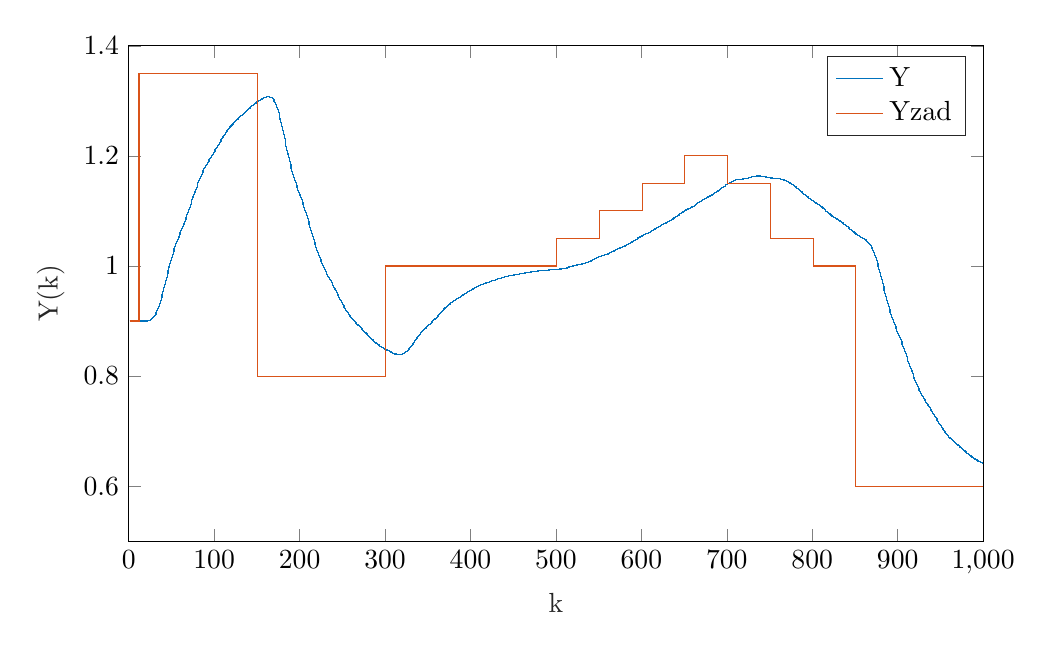
\begin{tikzpicture}

\begin{axis}[%
width=4.272in,
height=2.477in,
at={(0.717in,0.437in)},
scale only axis,
xmin=0,
xmax=1000,
xlabel style={font=\color{white!15!black}},
xlabel={k},
ymin=0.5,
ymax=1.4,
ylabel style={font=\color{white!15!black}},
ylabel={Y(k)},
axis background/.style={fill=white},
legend style={legend cell align=left, align=left, draw=white!15!black}
]
\addplot[const plot, color=mycolor1] table[row sep=crcr] {%
1	0.9\\
2	0.9\\
3	0.9\\
4	0.9\\
5	0.9\\
6	0.9\\
7	0.9\\
8	0.9\\
9	0.9\\
10	0.9\\
11	0.9\\
12	0.9\\
13	0.9\\
14	0.9\\
15	0.9\\
16	0.9\\
17	0.9\\
18	0.9\\
19	0.9\\
20	0.9\\
21	0.9\\
22	0.9003968325\\
23	0.90110505465075\\
24	0.901754499448244\\
25	0.902462381771257\\
26	0.903327432799628\\
27	0.904432123866198\\
28	0.90584465078664\\
29	0.907620702973639\\
30	0.909805039263915\\
31	0.912432890235655\\
32	0.915498096835601\\
33	0.918965853372063\\
34	0.922837193061285\\
35	0.927128134502026\\
36	0.931831863484165\\
37	0.936923734431968\\
38	0.942365468215513\\
39	0.948108657807613\\
40	0.954097679116409\\
41	0.960272091866446\\
42	0.966571366665219\\
43	0.97294065568034\\
44	0.979329694247744\\
45	0.985688442749354\\
46	0.991967881999957\\
47	0.998123300499065\\
48	1.00411656075767\\
49	1.00991755516541\\
50	1.01550502606484\\
51	1.0208668943165\\
52	1.0259999844607\\
53	1.03090892615053\\
54	1.03560478986773\\
55	1.04010429107047\\
56	1.04442934161618\\
57	1.04860630459408\\
58	1.05266486491142\\
59	1.05663669420945\\
60	1.0605540422755\\
61	1.06444835015091\\
62	1.06834897017567\\
63	1.07228209848007\\
64	1.07626998780362\\
65	1.08033038969881\\
66	1.08447613243709\\
67	1.08871482012883\\
68	1.09304869808435\\
69	1.09747471797913\\
70	1.10198480880132\\
71	1.10656634102768\\
72	1.11120275821343\\
73	1.11587433707758\\
74	1.12055902663016\\
75	1.12523332003065\\
76	1.12987312861239\\
77	1.13445463865313\\
78	1.13895513044294\\
79	1.14335373448336\\
80	1.14763209849147\\
81	1.15177494149719\\
82	1.1557704762483\\
83	1.15961068776104\\
84	1.16329146381875\\
85	1.16681258108326\\
86	1.17017755613573\\
87	1.17339337378769\\
88	1.17647010700276\\
89	1.17942044510106\\
90	1.18225914955358\\
91	1.18500245899432\\
92	1.18766746662559\\
93	1.19027149370736\\
94	1.19283148214764\\
95	1.19536342734718\\
96	1.1978818696875\\
97	1.20039945985026\\
98	1.20292660984184\\
99	1.20547123822702\\
100	1.2080386145976\\
101	1.21063130471987\\
102	1.21324921421263\\
103	1.21588972514576\\
104	1.21854791678215\\
105	1.22121685897705\\
106	1.22388796462404\\
107	1.22655138605161\\
108	1.2291964394166\\
109	1.23181204087031\\
110	1.23438713855422\\
111	1.2369111252862\\
112	1.23937421809208\\
113	1.24176779247258\\
114	1.24408466140287\\
115	1.24631929145305\\
116	1.24846795098764\\
117	1.2505287880408\\
118	1.2525018380675\\
119	1.25438896424786\\
120	1.25619373529506\\
121	1.25792124771947\\
122	1.25957790117795\\
123	1.26117113684122\\
124	1.26270914961122\\
125	1.26420058549763\\
126	1.26565423551553\\
127	1.26707873711107\\
128	1.26848229338989\\
129	1.2698724193567\\
130	1.27125572302791\\
131	1.27263772771127\\
132	1.27402274002252\\
133	1.27541376639511\\
134	1.27681247900324\\
135	1.27821923022645\\
136	1.27963311309799\\
137	1.28105206365459\\
138	1.28247299979045\\
139	1.28389199015027\\
140	1.285304445803\\
141	1.28670532693611\\
142	1.2880893566037\\
143	1.28945123364788\\
144	1.29078583727327\\
145	1.29208841636796\\
146	1.29335475749583\\
147	1.29458132649851\\
148	1.29576537979462\\
149	1.29690504270447\\
150	1.29799935341126\\
151	1.29904827244758\\
152	1.30005265882428\\
153	1.30101421505558\\
154	1.30193540434301\\
155	1.30281934403149\\
156	1.30366968011989\\
157	1.30449044807919\\
158	1.30528592549637\\
159	1.30606048211984\\
160	1.30681843273953\\
161	1.30716369682455\\
162	1.30717941725438\\
163	1.30722458102453\\
164	1.30716381414196\\
165	1.30688317044968\\
166	1.30628742896576\\
167	1.30529770217837\\
168	1.30384932587905\\
169	1.3018900031321\\
170	1.2993781767954\\
171	1.29631499574341\\
172	1.2927319090087\\
173	1.2886269424304\\
174	1.28398656026348\\
175	1.2788234391972\\
176	1.27317069285459\\
177	1.26707704408256\\
178	1.26060280915345\\
179	1.25381657523541\\
180	1.24679246780261\\
181	1.23960513258249\\
182	1.23232366515491\\
183	1.22501234716547\\
184	1.21773453022157\\
185	1.21055133104061\\
186	1.20351794537139\\
187	1.19668112903149\\
188	1.19007760151277\\
189	1.18373317014001\\
190	1.17766240879857\\
191	1.1718689880777\\
192	1.16634687067229\\
193	1.16108181655011\\
194	1.15605237449859\\
195	1.15123058867484\\
196	1.14658305274622\\
197	1.14207237455282\\
198	1.13765885013809\\
199	1.13330219926585\\
200	1.12896325677001\\
201	1.12460552784681\\
202	1.12019649736667\\
203	1.1157086215278\\
204	1.11112004815648\\
205	1.10641515354477\\
206	1.10158490527865\\
207	1.09662700428\\
208	1.0915457746403\\
209	1.08635180023695\\
210	1.08106132727517\\
211	1.07569546592208\\
212	1.07027923752917\\
213	1.0648405244653\\
214	1.05940897646577\\
215	1.05401491185706\\
216	1.04868824109481\\
217	1.04345744096653\\
218	1.03834861185122\\
219	1.0333846504378\\
220	1.02858456628647\\
221	1.02396296422117\\
222	1.01952970649721\\
223	1.01528975940691\\
224	1.01124321991638\\
225	1.00738551114763\\
226	1.00370773142582\\
227	1.00019713861747\\
228	0.99683774830098\\
229	0.993611021036291\\
230	0.990496611290706\\
231	0.987473148899105\\
232	0.984519023523776\\
233	0.981613143560161\\
234	0.978735643274665\\
235	0.975868515342502\\
236	0.97299614989132\\
237	0.970105765306768\\
238	0.967187720337565\\
239	0.964235701468817\\
240	0.961246784068318\\
241	0.958221370319641\\
242	0.955163011260938\\
243	0.952078124157511\\
244	0.948975619765714\\
245	0.945866456655265\\
246	0.94276314158254\\
247	0.939679195955599\\
248	0.936628608741493\\
249	0.93362529577704\\
250	0.930682584392817\\
251	0.927812740593989\\
252	0.92502655382839\\
253	0.922332991702936\\
254	0.919738933997245\\
255	0.917248992097394\\
256	0.91486541666791\\
257	0.912588093123838\\
258	0.910414621370712\\
259	0.908340473446145\\
260	0.906359220206614\\
261	0.904462816127511\\
262	0.902641929679672\\
263	0.900886305650784\\
264	0.8991851452154\\
265	0.897527489522673\\
266	0.895902593045374\\
267	0.894300273878\\
268	0.892711229530689\\
269	0.891127308472649\\
270	0.889541729658373\\
271	0.887949244441043\\
272	0.886346237555857\\
273	0.884730766156806\\
274	0.88310253813116\\
275	0.881462833019366\\
276	0.879814370764858\\
277	0.878161135149582\\
278	0.876508160089889\\
279	0.874861287940593\\
280	0.873226909562449\\
281	0.871611696144242\\
282	0.870022332642392\\
283	0.868465262228174\\
284	0.866946450346648\\
285	0.865471175933068\\
286	0.864043856050893\\
287	0.862667908765514\\
288	0.861345657508032\\
289	0.860078278573851\\
290	0.858865791800825\\
291	0.857707092937426\\
292	0.856600024794666\\
293	0.855541483021535\\
294	0.854527551290118\\
295	0.853553659852368\\
296	0.852614760855281\\
297	0.851705513484875\\
298	0.850820471952338\\
299	0.84995426952895\\
300	0.849101792262645\\
301	0.848258336643261\\
302	0.847419746294486\\
303	0.846582523721994\\
304	0.84574391419954\\
305	0.844901959986352\\
306	0.844055524198045\\
307	0.843204284758678\\
308	0.842348699905252\\
309	0.841489947663514\\
310	0.840629842535724\\
311	0.840169094662738\\
312	0.840027359635076\\
313	0.839805903831571\\
314	0.839567209155041\\
315	0.83936480474152\\
316	0.839244206365335\\
317	0.839243750798437\\
318	0.839395340436324\\
319	0.839725111766168\\
320	0.840254039536307\\
321	0.840965251242341\\
322	0.841815990385479\\
323	0.842804380409815\\
324	0.843952805469557\\
325	0.845270429284305\\
326	0.846755821961687\\
327	0.848399199457051\\
328	0.850184327694026\\
329	0.852090136165507\\
330	0.854092079575684\\
331	0.856166053544525\\
332	0.858293559373643\\
333	0.860459927998672\\
334	0.862648812483973\\
335	0.864841570203845\\
336	0.867019426091502\\
337	0.869165057096226\\
338	0.871263707431921\\
339	0.873303926457666\\
340	0.875278006001206\\
341	0.877181949883109\\
342	0.879014709072526\\
343	0.880777223160516\\
344	0.882472141796327\\
345	0.884104055543816\\
346	0.885679576426447\\
347	0.887207109824139\\
348	0.888696427994394\\
349	0.890158129663874\\
350	0.891603049252957\\
351	0.893041681803541\\
352	0.894483719627462\\
353	0.895937764786653\\
354	0.897411160909335\\
355	0.898909838051168\\
356	0.900438141685211\\
357	0.901998684545975\\
358	0.90359226015397\\
359	0.905217837966332\\
360	0.906872646603919\\
361	0.908552340683483\\
362	0.910251234068291\\
363	0.911962570966477\\
364	0.913678808404027\\
365	0.915391899148136\\
366	0.917093575864466\\
367	0.918775636276858\\
368	0.920430222821914\\
369	0.922050086094013\\
370	0.923628820126828\\
371	0.925161058368271\\
372	0.926642621853169\\
373	0.928070615443676\\
374	0.929443472725517\\
375	0.930760953011266\\
376	0.93202409432847\\
377	0.933235125828997\\
378	0.934397343260897\\
379	0.935514952183391\\
380	0.936592885001724\\
381	0.937636599219598\\
382	0.938651865245467\\
383	0.93964455239024\\
384	0.940620421246598\\
385	0.941584929632738\\
386	0.942543058110608\\
387	0.943499160027043\\
388	0.944456840079157\\
389	0.945418864441198\\
390	0.946387104412926\\
391	0.947362514345214\\
392	0.948345143313419\\
393	0.949334178730906\\
394	0.950328018934164\\
395	0.951324370821061\\
396	0.9523203679239\\
397	0.953312703830763\\
398	0.954297775593714\\
399	0.955271831656608\\
400	0.956231118895027\\
401	0.957172023592017\\
402	0.95809120157877\\
403	0.958985693341087\\
404	0.959853020607133\\
405	0.960691261752121\\
406	0.961499104236219\\
407	0.962275873190419\\
408	0.9630215361472\\
409	0.963736684751766\\
410	0.96442249506354\\
411	0.965080668745633\\
412	0.965713358022552\\
413	0.966323077745515\\
414	0.966912608226528\\
415	0.967484892678643\\
416	0.968042933129712\\
417	0.968589688566427\\
418	0.969127978825942\\
419	0.969660397399219\\
420	0.970189235861091\\
421	0.970716422116399\\
422	0.971243474070611\\
423	0.971771469719207\\
424	0.972301034025811\\
425	0.972832342347339\\
426	0.973365139586878\\
427	0.973898773731139\\
428	0.974432241975527\\
429	0.974964247269264\\
430	0.975493262835007\\
431	0.976017602037695\\
432	0.97653549089826\\
433	0.977045140567746\\
434	0.97754481719178\\
435	0.978032906796037\\
436	0.978507973099932\\
437	0.978968806504891\\
438	0.979414462890818\\
439	0.979844291273657\\
440	0.980257949812176\\
441	0.980655410087131\\
442	0.98103694999534\\
443	0.981403135990794\\
444	0.981754795752179\\
445	0.982092982650503\\
446	0.982418933623735\\
447	0.982734022231702\\
448	0.983039708760909\\
449	0.983337489274906\\
450	0.983628845463454\\
451	0.983915197037351\\
452	0.98419785825193\\
453	0.984477999929074\\
454	0.984756618094831\\
455	0.985034510067923\\
456	0.985312258534895\\
457	0.985590223841668\\
458	0.985868544430038\\
459	0.986147145061628\\
460	0.98642575221052\\
461	0.986703915777452\\
462	0.986981036089827\\
463	0.987256395007808\\
464	0.987529189860735\\
465	0.987798568891391\\
466	0.988063666887806\\
467	0.988323639731228\\
468	0.988577696680858\\
469	0.988825129345951\\
470	0.989065336457574\\
471	0.989297843738771\\
472	0.989522318375325\\
473	0.989738577801861\\
474	0.989946592731781\\
475	0.990146484566763\\
476	0.990338517515298\\
477	0.990523085923603\\
478	0.990700697470936\\
479	0.990871953000652\\
480	0.991037523845198\\
481	0.991198127556078\\
482	0.991354502968001\\
483	0.99150738551097\\
484	0.991657483636728\\
485	0.991805457149996\\
486	0.99195189813403\\
487	0.992097315038895\\
488	0.992242120364734\\
489	0.992386622226472\\
490	0.992531019936621\\
491	0.992675403594489\\
492	0.992819757528406\\
493	0.992963967307301\\
494	0.993107829923245\\
495	0.993251066650795\\
496	0.993393338014796\\
497	0.993534260247401\\
498	0.993673422588261\\
499	0.993810404779147\\
500	0.993944794124629\\
501	0.99407620153232\\
502	0.994204276007057\\
503	0.994328717150409\\
504	0.994449285306534\\
505	0.994565809094043\\
506	0.994678190167261\\
507	0.994786405155133\\
508	0.994890504828404\\
509	0.994990610641852\\
510	0.995086908885376\\
511	0.995576320281363\\
512	0.996373384114822\\
513	0.997056856627257\\
514	0.997652839785233\\
515	0.998184012720492\\
516	0.998670007498053\\
517	0.999127744934178\\
518	0.999571734880995\\
519	1.00001434495842\\
520	1.00046604130442\\
521	1.00090250944675\\
522	1.00127650821095\\
523	1.0015858198777\\
524	1.00185870519926\\
525	1.00211644344964\\
526	1.00237451129508\\
527	1.00264359443392\\
528	1.00293045372561\\
529	1.00323866481912\\
530	1.00356924790285\\
531	1.00392396324233\\
532	1.00430993647707\\
533	1.00473730119126\\
534	1.00521289410927\\
535	1.00573874175239\\
536	1.00631352098964\\
537	1.00693371374279\\
538	1.00759450858742\\
539	1.00829049389687\\
540	1.00901618023572\\
541	1.00976615340582\\
542	1.01053456799302\\
543	1.01131451329682\\
544	1.01209814152972\\
545	1.01287740668452\\
546	1.0136447383078\\
547	1.01439344764917\\
548	1.01511793444369\\
549	1.01581374868606\\
550	1.01647755031866\\
551	1.01710701960353\\
552	1.01770080634101\\
553	1.01825857732303\\
554	1.01878110040905\\
555	1.01927025124573\\
556	1.01972890636205\\
557	1.02016075941615\\
558	1.02057010446154\\
559	1.02096161646853\\
560	1.02134014894019\\
561	1.02210452711472\\
562	1.0231686533107\\
563	1.02411388033609\\
564	1.02497152632599\\
565	1.02576872843422\\
566	1.02652873592204\\
567	1.02727119274802\\
568	1.02801241990539\\
569	1.02876570092291\\
570	1.02954156963095\\
571	1.0303152279108\\
572	1.0310388789943\\
573	1.0317096173736\\
574	1.0323544237142\\
575	1.03299261216525\\
576	1.03363719623706\\
577	1.03429608179113\\
578	1.03497310437641\\
579	1.03566892538143\\
580	1.03638179985561\\
581	1.03711097021104\\
582	1.03786131833729\\
583	1.03864100027169\\
584	1.03945517760363\\
585	1.04030458173921\\
586	1.04118703782354\\
587	1.0420986482806\\
588	1.04303469293783\\
589	1.04399029493723\\
590	1.04496089494533\\
591	1.04594234152182\\
592	1.04693031770527\\
593	1.04791964447353\\
594	1.04890434954974\\
595	1.04987834266631\\
596	1.05083601969436\\
597	1.05177259750311\\
598	1.05268425308141\\
599	1.05356812540787\\
600	1.05442222602796\\
601	1.05524531299143\\
602	1.05603681669851\\
603	1.05679687588109\\
604	1.05752642048665\\
605	1.05822718673863\\
606	1.05890162816246\\
607	1.05955275920072\\
608	1.06018397437369\\
609	1.06079887163916\\
610	1.06140109777379\\
611	1.06238815529502\\
612	1.06367267808548\\
613	1.06483479509767\\
614	1.06590458609383\\
615	1.06690806065741\\
616	1.06786748757226\\
617	1.06880170721111\\
618	1.06972643631653\\
619	1.0706545679902\\
620	1.07159646572185\\
621	1.07252738232499\\
622	1.07339977939622\\
623	1.07421119225364\\
624	1.07498920795452\\
625	1.07575389159591\\
626	1.07651912025515\\
627	1.07729374153833\\
628	1.07808257524797\\
629	1.07888727392648\\
630	1.07970705637811\\
631	1.08054206928726\\
632	1.08139801088139\\
633	1.08228374254525\\
634	1.08320500228119\\
635	1.08416295539202\\
636	1.08515571003377\\
637	1.08617949822132\\
638	1.08722957906351\\
639	1.0883009130564\\
640	1.08938864940792\\
641	1.09048823359354\\
642	1.09159485441299\\
643	1.09270277022996\\
644	1.09380540185966\\
645	1.09489603238126\\
646	1.09596843550646\\
647	1.09701723353714\\
648	1.09803805764719\\
649	1.09902756828703\\
650	1.0999833811087\\
651	1.10090395264316\\
652	1.10178851400379\\
653	1.10263711072739\\
654	1.10345068556976\\
655	1.10423108971657\\
656	1.10498098649525\\
657	1.10570368460722\\
658	1.10640294432696\\
659	1.10708278588701\\
660	1.10774731848689\\
661	1.10879426684647\\
662	1.11013625476138\\
663	1.11135373743873\\
664	1.11247740266507\\
665	1.11353380841378\\
666	1.11454570224341\\
667	1.11553232585545\\
668	1.11650971445948\\
669	1.11749099392267\\
670	1.1184866745911\\
671	1.11947209456598\\
672	1.12039978281921\\
673	1.12126731604091\\
674	1.12210224887935\\
675	1.12292452910398\\
676	1.12374784895551\\
677	1.12458082097511\\
678	1.12542799649262\\
679	1.12629074219102\\
680	1.1271679885211\\
681	1.12805960294725\\
682	1.12897101871664\\
683	1.12991084840482\\
684	1.13088460379443\\
685	1.13189325717508\\
686	1.13293476610728\\
687	1.13400526012467\\
688	1.13509994650245\\
689	1.13621378429167\\
690	1.13734196898248\\
691	1.13848003555344\\
692	1.13962330012502\\
693	1.14076618074463\\
694	1.14190228463933\\
695	1.14302510151463\\
696	1.1441286243791\\
697	1.1452076994052\\
698	1.14625817813512\\
699	1.1472769302977\\
700	1.14826176300142\\
701	1.1492113007963\\
702	1.15012491499655\\
703	1.15100276034006\\
704	1.15184585571573\\
705	1.1526560944107\\
706	1.15343614802474\\
707	1.15418930110183\\
708	1.15491925987001\\
709	1.15562996417528\\
710	1.15632542085964\\
711	1.15660953296027\\
712	1.15656562739792\\
713	1.15661695467116\\
714	1.15674276891108\\
715	1.15692504397472\\
716	1.15714802462289\\
717	1.15739784291573\\
718	1.15766220131747\\
719	1.15793011813117\\
720	1.15819172753006\\
721	1.15847150016088\\
722	1.15881694305253\\
723	1.15923053228696\\
724	1.15968365629161\\
725	1.1601539234925\\
726	1.16062416814294\\
727	1.16108161656035\\
728	1.16151718832924\\
729	1.16192490959913\\
730	1.1623014186716\\
731	1.1626427627249\\
732	1.16293978402222\\
733	1.16318045408291\\
734	1.16335621669888\\
735	1.16346359664284\\
736	1.16350282346908\\
737	1.16347672519449\\
738	1.16338984362053\\
739	1.16324773134106\\
740	1.163056397555\\
741	1.16282210804564\\
742	1.16255184080787\\
743	1.16225387495435\\
744	1.16193762008565\\
745	1.16161282781298\\
746	1.16128885812461\\
747	1.16097420775358\\
748	1.16067623811486\\
749	1.16040105304662\\
750	1.16015348687908\\
751	1.15993715228771\\
752	1.15975446034756\\
753	1.15960655226226\\
754	1.15949320284716\\
755	1.15941280941183\\
756	1.15936250305687\\
757	1.15933834616354\\
758	1.15933557188196\\
759	1.15934883425454\\
760	1.15937244746529\\
761	1.15900607376211\\
762	1.15833390341491\\
763	1.157766928442\\
764	1.15726160581972\\
765	1.15678047243207\\
766	1.15629166314418\\
767	1.15576845944938\\
768	1.15518885488097\\
769	1.15453513065448\\
770	1.15379343983219\\
771	1.15298631693775\\
772	1.15216029934633\\
773	1.15131842387498\\
774	1.15043591462256\\
775	1.14949773433263\\
776	1.14849672806443\\
777	1.14743201403219\\
778	1.14630759444943\\
779	1.14513116345229\\
780	1.14391309205334\\
781	1.14266282588095\\
782	1.14138405286393\\
783	1.14007687579086\\
784	1.13874381743319\\
785	1.13739096119269\\
786	1.13602619733521\\
787	1.13465790136206\\
788	1.13329396838876\\
789	1.13194113837472\\
790	1.13060455643133\\
791	1.12928774967432\\
792	1.12799329248697\\
793	1.12672361640726\\
794	1.12548108141797\\
795	1.12426747371202\\
796	1.12308360208697\\
797	1.12192917631291\\
798	1.12080287991332\\
799	1.11970256885595\\
800	1.11862554336144\\
801	1.11756883382064\\
802	1.1165294097582\\
803	1.11550425217048\\
804	1.11449035090926\\
805	1.11348473943144\\
806	1.11248460083501\\
807	1.11148740806793\\
808	1.11049105718672\\
809	1.10949396858202\\
810	1.1084951429369\\
811	1.10710085710149\\
812	1.10540272560453\\
813	1.10382439704228\\
814	1.10233945785245\\
815	1.10092555673665\\
816	1.09956393938571\\
817	1.09823901149092\\
818	1.09693792473891\\
819	1.09565018629839\\
820	1.09436729538197\\
821	1.09311522578388\\
822	1.09194203083433\\
823	1.09085003884519\\
824	1.08981097364837\\
825	1.08880358084663\\
826	1.0878123445037\\
827	1.08682639548319\\
828	1.08583858950236\\
829	1.08484473542966\\
830	1.08384295586982\\
831	1.08283042539599\\
832	1.08179885254763\\
833	1.08073696622068\\
834	1.0796368794415\\
835	1.07849559783094\\
836	1.07731355050408\\
837	1.07609344275047\\
838	1.074839372482\\
839	1.07355616104324\\
840	1.07224885647259\\
841	1.07092260231086\\
842	1.06958315289201\\
843	1.0682374967167\\
844	1.0668937037547\\
845	1.06556016022923\\
846	1.06424487209224\\
847	1.06295503833647\\
848	1.06169682351523\\
849	1.0604752737494\\
850	1.05929433277565\\
851	1.05815690557293\\
852	1.05706488288663\\
853	1.05601906989174\\
854	1.05501908305764\\
855	1.05406332999805\\
856	1.05314910792501\\
857	1.0522727830289\\
858	1.0514300064048\\
859	1.05061593612723\\
860	1.04982544564154\\
861	1.04866006194682\\
862	1.04720675699953\\
863	1.04583915201055\\
864	1.04444483292963\\
865	1.04292876302134\\
866	1.04121139574632\\
867	1.0392269724676\\
868	1.03692197637707\\
869	1.03425372271224\\
870	1.03118907127479\\
871	1.02773605986978\\
872	1.0239306788736\\
873	1.0197720691455\\
874	1.01524322831835\\
875	1.0103489406592\\
876	1.00511104002655\\
877	0.999564401455219\\
878	0.993753565771211\\
879	0.987729914538255\\
880	0.981549323160261\\
881	0.975267491456203\\
882	0.96893428242139\\
883	0.962594984024355\\
884	0.956294853322811\\
885	0.95007849318461\\
886	0.943986691587205\\
887	0.93805423455346\\
888	0.932308497231893\\
889	0.926768649650635\\
890	0.921445340872772\\
891	0.916340976806125\\
892	0.911450808238994\\
893	0.906764263645407\\
894	0.902265688195684\\
895	0.897934711556627\\
896	0.893746895133604\\
897	0.889674755244686\\
898	0.885688990620384\\
899	0.881759786331988\\
900	0.877858101313884\\
901	0.873956855501901\\
902	0.870031912293237\\
903	0.866062790490992\\
904	0.862033159520349\\
905	0.857931214455777\\
906	0.853749947312385\\
907	0.849487270131541\\
908	0.845145955558932\\
909	0.84073338738237\\
910	0.836261131649344\\
911	0.831744352136894\\
912	0.827201107038398\\
913	0.822651574187706\\
914	0.818117248789103\\
915	0.813620141617379\\
916	0.809181994337698\\
917	0.804823529652822\\
918	0.800563758943257\\
919	0.7964193716131\\
920	0.792404228186671\\
921	0.788528974721117\\
922	0.784800789892824\\
923	0.781223268538993\\
924	0.777796437951791\\
925	0.774516897955673\\
926	0.771378073162333\\
927	0.76837056416608\\
928	0.765482582427319\\
929	0.762700451198557\\
930	0.760009152682474\\
931	0.757392900138492\\
932	0.754835713139305\\
933	0.752321974791951\\
934	0.749836951486375\\
935	0.747367258334212\\
936	0.744901256450578\\
937	0.742429371293228\\
938	0.739944324358326\\
939	0.737441273705462\\
940	0.73491786205511\\
941	0.732374174491128\\
942	0.729812610978711\\
943	0.72723768181921\\
944	0.724655736650958\\
945	0.722074639548534\\
946	0.719503404120612\\
947	0.716951803273966\\
948	0.714429968540231\\
949	0.711947993588959\\
950	0.709515555801358\\
951	0.707141568583377\\
952	0.704833875497243\\
953	0.702598995349443\\
954	0.700441925171891\\
955	0.698366005668534\\
956	0.696372851274094\\
957	0.694462344581607\\
958	0.692632692624408\\
959	0.690880540417061\\
960	0.689201135328303\\
961	0.687588534328345\\
962	0.686035844964175\\
963	0.684535490099561\\
964	0.683079486027715\\
965	0.68165972352496\\
966	0.680268241748796\\
967	0.678897485564674\\
968	0.677540537872084\\
969	0.676191319743302\\
970	0.67484475263212\\
971	0.673496878496058\\
972	0.672144935342448\\
973	0.670787387394415\\
974	0.669423910716804\\
975	0.6680553366876\\
976	0.666683557096194\\
977	0.66531139585244\\
978	0.663942453265141\\
979	0.662580929570544\\
980	0.661231434845904\\
981	0.659898792625496\\
982	0.658587844451669\\
983	0.657303262255805\\
984	0.656049374895924\\
985	0.654830014408904\\
986	0.653648386601519\\
987	0.652506969545916\\
988	0.651407442404593\\
989	0.650350645831398\\
990	0.649336574021993\\
991	0.648364397360974\\
992	0.647432513571419\\
993	0.646538624349309\\
994	0.645679833687972\\
995	0.644852763487643\\
996	0.644053681617327\\
997	0.643278637357637\\
998	0.642523599104896\\
999	0.641784589352077\\
1000	0.641057812268653\\
};
\addlegendentry{Y}

\addplot[const plot, color=mycolor2] table[row sep=crcr] {%
1	0.9\\
2	0.9\\
3	0.9\\
4	0.9\\
5	0.9\\
6	0.9\\
7	0.9\\
8	0.9\\
9	0.9\\
10	0.9\\
11	0.9\\
12	1.35\\
13	1.35\\
14	1.35\\
15	1.35\\
16	1.35\\
17	1.35\\
18	1.35\\
19	1.35\\
20	1.35\\
21	1.35\\
22	1.35\\
23	1.35\\
24	1.35\\
25	1.35\\
26	1.35\\
27	1.35\\
28	1.35\\
29	1.35\\
30	1.35\\
31	1.35\\
32	1.35\\
33	1.35\\
34	1.35\\
35	1.35\\
36	1.35\\
37	1.35\\
38	1.35\\
39	1.35\\
40	1.35\\
41	1.35\\
42	1.35\\
43	1.35\\
44	1.35\\
45	1.35\\
46	1.35\\
47	1.35\\
48	1.35\\
49	1.35\\
50	1.35\\
51	1.35\\
52	1.35\\
53	1.35\\
54	1.35\\
55	1.35\\
56	1.35\\
57	1.35\\
58	1.35\\
59	1.35\\
60	1.35\\
61	1.35\\
62	1.35\\
63	1.35\\
64	1.35\\
65	1.35\\
66	1.35\\
67	1.35\\
68	1.35\\
69	1.35\\
70	1.35\\
71	1.35\\
72	1.35\\
73	1.35\\
74	1.35\\
75	1.35\\
76	1.35\\
77	1.35\\
78	1.35\\
79	1.35\\
80	1.35\\
81	1.35\\
82	1.35\\
83	1.35\\
84	1.35\\
85	1.35\\
86	1.35\\
87	1.35\\
88	1.35\\
89	1.35\\
90	1.35\\
91	1.35\\
92	1.35\\
93	1.35\\
94	1.35\\
95	1.35\\
96	1.35\\
97	1.35\\
98	1.35\\
99	1.35\\
100	1.35\\
101	1.35\\
102	1.35\\
103	1.35\\
104	1.35\\
105	1.35\\
106	1.35\\
107	1.35\\
108	1.35\\
109	1.35\\
110	1.35\\
111	1.35\\
112	1.35\\
113	1.35\\
114	1.35\\
115	1.35\\
116	1.35\\
117	1.35\\
118	1.35\\
119	1.35\\
120	1.35\\
121	1.35\\
122	1.35\\
123	1.35\\
124	1.35\\
125	1.35\\
126	1.35\\
127	1.35\\
128	1.35\\
129	1.35\\
130	1.35\\
131	1.35\\
132	1.35\\
133	1.35\\
134	1.35\\
135	1.35\\
136	1.35\\
137	1.35\\
138	1.35\\
139	1.35\\
140	1.35\\
141	1.35\\
142	1.35\\
143	1.35\\
144	1.35\\
145	1.35\\
146	1.35\\
147	1.35\\
148	1.35\\
149	1.35\\
150	1.35\\
151	0.8\\
152	0.8\\
153	0.8\\
154	0.8\\
155	0.8\\
156	0.8\\
157	0.8\\
158	0.8\\
159	0.8\\
160	0.8\\
161	0.8\\
162	0.8\\
163	0.8\\
164	0.8\\
165	0.8\\
166	0.8\\
167	0.8\\
168	0.8\\
169	0.8\\
170	0.8\\
171	0.8\\
172	0.8\\
173	0.8\\
174	0.8\\
175	0.8\\
176	0.8\\
177	0.8\\
178	0.8\\
179	0.8\\
180	0.8\\
181	0.8\\
182	0.8\\
183	0.8\\
184	0.8\\
185	0.8\\
186	0.8\\
187	0.8\\
188	0.8\\
189	0.8\\
190	0.8\\
191	0.8\\
192	0.8\\
193	0.8\\
194	0.8\\
195	0.8\\
196	0.8\\
197	0.8\\
198	0.8\\
199	0.8\\
200	0.8\\
201	0.8\\
202	0.8\\
203	0.8\\
204	0.8\\
205	0.8\\
206	0.8\\
207	0.8\\
208	0.8\\
209	0.8\\
210	0.8\\
211	0.8\\
212	0.8\\
213	0.8\\
214	0.8\\
215	0.8\\
216	0.8\\
217	0.8\\
218	0.8\\
219	0.8\\
220	0.8\\
221	0.8\\
222	0.8\\
223	0.8\\
224	0.8\\
225	0.8\\
226	0.8\\
227	0.8\\
228	0.8\\
229	0.8\\
230	0.8\\
231	0.8\\
232	0.8\\
233	0.8\\
234	0.8\\
235	0.8\\
236	0.8\\
237	0.8\\
238	0.8\\
239	0.8\\
240	0.8\\
241	0.8\\
242	0.8\\
243	0.8\\
244	0.8\\
245	0.8\\
246	0.8\\
247	0.8\\
248	0.8\\
249	0.8\\
250	0.8\\
251	0.8\\
252	0.8\\
253	0.8\\
254	0.8\\
255	0.8\\
256	0.8\\
257	0.8\\
258	0.8\\
259	0.8\\
260	0.8\\
261	0.8\\
262	0.8\\
263	0.8\\
264	0.8\\
265	0.8\\
266	0.8\\
267	0.8\\
268	0.8\\
269	0.8\\
270	0.8\\
271	0.8\\
272	0.8\\
273	0.8\\
274	0.8\\
275	0.8\\
276	0.8\\
277	0.8\\
278	0.8\\
279	0.8\\
280	0.8\\
281	0.8\\
282	0.8\\
283	0.8\\
284	0.8\\
285	0.8\\
286	0.8\\
287	0.8\\
288	0.8\\
289	0.8\\
290	0.8\\
291	0.8\\
292	0.8\\
293	0.8\\
294	0.8\\
295	0.8\\
296	0.8\\
297	0.8\\
298	0.8\\
299	0.8\\
300	0.8\\
301	1\\
302	1\\
303	1\\
304	1\\
305	1\\
306	1\\
307	1\\
308	1\\
309	1\\
310	1\\
311	1\\
312	1\\
313	1\\
314	1\\
315	1\\
316	1\\
317	1\\
318	1\\
319	1\\
320	1\\
321	1\\
322	1\\
323	1\\
324	1\\
325	1\\
326	1\\
327	1\\
328	1\\
329	1\\
330	1\\
331	1\\
332	1\\
333	1\\
334	1\\
335	1\\
336	1\\
337	1\\
338	1\\
339	1\\
340	1\\
341	1\\
342	1\\
343	1\\
344	1\\
345	1\\
346	1\\
347	1\\
348	1\\
349	1\\
350	1\\
351	1\\
352	1\\
353	1\\
354	1\\
355	1\\
356	1\\
357	1\\
358	1\\
359	1\\
360	1\\
361	1\\
362	1\\
363	1\\
364	1\\
365	1\\
366	1\\
367	1\\
368	1\\
369	1\\
370	1\\
371	1\\
372	1\\
373	1\\
374	1\\
375	1\\
376	1\\
377	1\\
378	1\\
379	1\\
380	1\\
381	1\\
382	1\\
383	1\\
384	1\\
385	1\\
386	1\\
387	1\\
388	1\\
389	1\\
390	1\\
391	1\\
392	1\\
393	1\\
394	1\\
395	1\\
396	1\\
397	1\\
398	1\\
399	1\\
400	1\\
401	1\\
402	1\\
403	1\\
404	1\\
405	1\\
406	1\\
407	1\\
408	1\\
409	1\\
410	1\\
411	1\\
412	1\\
413	1\\
414	1\\
415	1\\
416	1\\
417	1\\
418	1\\
419	1\\
420	1\\
421	1\\
422	1\\
423	1\\
424	1\\
425	1\\
426	1\\
427	1\\
428	1\\
429	1\\
430	1\\
431	1\\
432	1\\
433	1\\
434	1\\
435	1\\
436	1\\
437	1\\
438	1\\
439	1\\
440	1\\
441	1\\
442	1\\
443	1\\
444	1\\
445	1\\
446	1\\
447	1\\
448	1\\
449	1\\
450	1\\
451	1\\
452	1\\
453	1\\
454	1\\
455	1\\
456	1\\
457	1\\
458	1\\
459	1\\
460	1\\
461	1\\
462	1\\
463	1\\
464	1\\
465	1\\
466	1\\
467	1\\
468	1\\
469	1\\
470	1\\
471	1\\
472	1\\
473	1\\
474	1\\
475	1\\
476	1\\
477	1\\
478	1\\
479	1\\
480	1\\
481	1\\
482	1\\
483	1\\
484	1\\
485	1\\
486	1\\
487	1\\
488	1\\
489	1\\
490	1\\
491	1\\
492	1\\
493	1\\
494	1\\
495	1\\
496	1\\
497	1\\
498	1\\
499	1\\
500	1\\
501	1.05\\
502	1.05\\
503	1.05\\
504	1.05\\
505	1.05\\
506	1.05\\
507	1.05\\
508	1.05\\
509	1.05\\
510	1.05\\
511	1.05\\
512	1.05\\
513	1.05\\
514	1.05\\
515	1.05\\
516	1.05\\
517	1.05\\
518	1.05\\
519	1.05\\
520	1.05\\
521	1.05\\
522	1.05\\
523	1.05\\
524	1.05\\
525	1.05\\
526	1.05\\
527	1.05\\
528	1.05\\
529	1.05\\
530	1.05\\
531	1.05\\
532	1.05\\
533	1.05\\
534	1.05\\
535	1.05\\
536	1.05\\
537	1.05\\
538	1.05\\
539	1.05\\
540	1.05\\
541	1.05\\
542	1.05\\
543	1.05\\
544	1.05\\
545	1.05\\
546	1.05\\
547	1.05\\
548	1.05\\
549	1.05\\
550	1.05\\
551	1.1\\
552	1.1\\
553	1.1\\
554	1.1\\
555	1.1\\
556	1.1\\
557	1.1\\
558	1.1\\
559	1.1\\
560	1.1\\
561	1.1\\
562	1.1\\
563	1.1\\
564	1.1\\
565	1.1\\
566	1.1\\
567	1.1\\
568	1.1\\
569	1.1\\
570	1.1\\
571	1.1\\
572	1.1\\
573	1.1\\
574	1.1\\
575	1.1\\
576	1.1\\
577	1.1\\
578	1.1\\
579	1.1\\
580	1.1\\
581	1.1\\
582	1.1\\
583	1.1\\
584	1.1\\
585	1.1\\
586	1.1\\
587	1.1\\
588	1.1\\
589	1.1\\
590	1.1\\
591	1.1\\
592	1.1\\
593	1.1\\
594	1.1\\
595	1.1\\
596	1.1\\
597	1.1\\
598	1.1\\
599	1.1\\
600	1.1\\
601	1.15\\
602	1.15\\
603	1.15\\
604	1.15\\
605	1.15\\
606	1.15\\
607	1.15\\
608	1.15\\
609	1.15\\
610	1.15\\
611	1.15\\
612	1.15\\
613	1.15\\
614	1.15\\
615	1.15\\
616	1.15\\
617	1.15\\
618	1.15\\
619	1.15\\
620	1.15\\
621	1.15\\
622	1.15\\
623	1.15\\
624	1.15\\
625	1.15\\
626	1.15\\
627	1.15\\
628	1.15\\
629	1.15\\
630	1.15\\
631	1.15\\
632	1.15\\
633	1.15\\
634	1.15\\
635	1.15\\
636	1.15\\
637	1.15\\
638	1.15\\
639	1.15\\
640	1.15\\
641	1.15\\
642	1.15\\
643	1.15\\
644	1.15\\
645	1.15\\
646	1.15\\
647	1.15\\
648	1.15\\
649	1.15\\
650	1.15\\
651	1.2\\
652	1.2\\
653	1.2\\
654	1.2\\
655	1.2\\
656	1.2\\
657	1.2\\
658	1.2\\
659	1.2\\
660	1.2\\
661	1.2\\
662	1.2\\
663	1.2\\
664	1.2\\
665	1.2\\
666	1.2\\
667	1.2\\
668	1.2\\
669	1.2\\
670	1.2\\
671	1.2\\
672	1.2\\
673	1.2\\
674	1.2\\
675	1.2\\
676	1.2\\
677	1.2\\
678	1.2\\
679	1.2\\
680	1.2\\
681	1.2\\
682	1.2\\
683	1.2\\
684	1.2\\
685	1.2\\
686	1.2\\
687	1.2\\
688	1.2\\
689	1.2\\
690	1.2\\
691	1.2\\
692	1.2\\
693	1.2\\
694	1.2\\
695	1.2\\
696	1.2\\
697	1.2\\
698	1.2\\
699	1.2\\
700	1.2\\
701	1.15\\
702	1.15\\
703	1.15\\
704	1.15\\
705	1.15\\
706	1.15\\
707	1.15\\
708	1.15\\
709	1.15\\
710	1.15\\
711	1.15\\
712	1.15\\
713	1.15\\
714	1.15\\
715	1.15\\
716	1.15\\
717	1.15\\
718	1.15\\
719	1.15\\
720	1.15\\
721	1.15\\
722	1.15\\
723	1.15\\
724	1.15\\
725	1.15\\
726	1.15\\
727	1.15\\
728	1.15\\
729	1.15\\
730	1.15\\
731	1.15\\
732	1.15\\
733	1.15\\
734	1.15\\
735	1.15\\
736	1.15\\
737	1.15\\
738	1.15\\
739	1.15\\
740	1.15\\
741	1.15\\
742	1.15\\
743	1.15\\
744	1.15\\
745	1.15\\
746	1.15\\
747	1.15\\
748	1.15\\
749	1.15\\
750	1.15\\
751	1.05\\
752	1.05\\
753	1.05\\
754	1.05\\
755	1.05\\
756	1.05\\
757	1.05\\
758	1.05\\
759	1.05\\
760	1.05\\
761	1.05\\
762	1.05\\
763	1.05\\
764	1.05\\
765	1.05\\
766	1.05\\
767	1.05\\
768	1.05\\
769	1.05\\
770	1.05\\
771	1.05\\
772	1.05\\
773	1.05\\
774	1.05\\
775	1.05\\
776	1.05\\
777	1.05\\
778	1.05\\
779	1.05\\
780	1.05\\
781	1.05\\
782	1.05\\
783	1.05\\
784	1.05\\
785	1.05\\
786	1.05\\
787	1.05\\
788	1.05\\
789	1.05\\
790	1.05\\
791	1.05\\
792	1.05\\
793	1.05\\
794	1.05\\
795	1.05\\
796	1.05\\
797	1.05\\
798	1.05\\
799	1.05\\
800	1.05\\
801	1\\
802	1\\
803	1\\
804	1\\
805	1\\
806	1\\
807	1\\
808	1\\
809	1\\
810	1\\
811	1\\
812	1\\
813	1\\
814	1\\
815	1\\
816	1\\
817	1\\
818	1\\
819	1\\
820	1\\
821	1\\
822	1\\
823	1\\
824	1\\
825	1\\
826	1\\
827	1\\
828	1\\
829	1\\
830	1\\
831	1\\
832	1\\
833	1\\
834	1\\
835	1\\
836	1\\
837	1\\
838	1\\
839	1\\
840	1\\
841	1\\
842	1\\
843	1\\
844	1\\
845	1\\
846	1\\
847	1\\
848	1\\
849	1\\
850	1\\
851	0.6\\
852	0.6\\
853	0.6\\
854	0.6\\
855	0.6\\
856	0.6\\
857	0.6\\
858	0.6\\
859	0.6\\
860	0.6\\
861	0.6\\
862	0.6\\
863	0.6\\
864	0.6\\
865	0.6\\
866	0.6\\
867	0.6\\
868	0.6\\
869	0.6\\
870	0.6\\
871	0.6\\
872	0.6\\
873	0.6\\
874	0.6\\
875	0.6\\
876	0.6\\
877	0.6\\
878	0.6\\
879	0.6\\
880	0.6\\
881	0.6\\
882	0.6\\
883	0.6\\
884	0.6\\
885	0.6\\
886	0.6\\
887	0.6\\
888	0.6\\
889	0.6\\
890	0.6\\
891	0.6\\
892	0.6\\
893	0.6\\
894	0.6\\
895	0.6\\
896	0.6\\
897	0.6\\
898	0.6\\
899	0.6\\
900	0.6\\
901	0.6\\
902	0.6\\
903	0.6\\
904	0.6\\
905	0.6\\
906	0.6\\
907	0.6\\
908	0.6\\
909	0.6\\
910	0.6\\
911	0.6\\
912	0.6\\
913	0.6\\
914	0.6\\
915	0.6\\
916	0.6\\
917	0.6\\
918	0.6\\
919	0.6\\
920	0.6\\
921	0.6\\
922	0.6\\
923	0.6\\
924	0.6\\
925	0.6\\
926	0.6\\
927	0.6\\
928	0.6\\
929	0.6\\
930	0.6\\
931	0.6\\
932	0.6\\
933	0.6\\
934	0.6\\
935	0.6\\
936	0.6\\
937	0.6\\
938	0.6\\
939	0.6\\
940	0.6\\
941	0.6\\
942	0.6\\
943	0.6\\
944	0.6\\
945	0.6\\
946	0.6\\
947	0.6\\
948	0.6\\
949	0.6\\
950	0.6\\
951	0.6\\
952	0.6\\
953	0.6\\
954	0.6\\
955	0.6\\
956	0.6\\
957	0.6\\
958	0.6\\
959	0.6\\
960	0.6\\
961	0.6\\
962	0.6\\
963	0.6\\
964	0.6\\
965	0.6\\
966	0.6\\
967	0.6\\
968	0.6\\
969	0.6\\
970	0.6\\
971	0.6\\
972	0.6\\
973	0.6\\
974	0.6\\
975	0.6\\
976	0.6\\
977	0.6\\
978	0.6\\
979	0.6\\
980	0.6\\
981	0.6\\
982	0.6\\
983	0.6\\
984	0.6\\
985	0.6\\
986	0.6\\
987	0.6\\
988	0.6\\
989	0.6\\
990	0.6\\
991	0.6\\
992	0.6\\
993	0.6\\
994	0.6\\
995	0.6\\
996	0.6\\
997	0.6\\
998	0.6\\
999	0.6\\
1000	0.6\\
};
\addlegendentry{Yzad}

\end{axis}
\end{tikzpicture}%
\caption{Śledzenie wartości zadanej dla parametrów ZN}
\end{figure}

Wskaźnik jakości regulacji:

\begin{equation}
E = 36,0711
\end{equation}

Zmieniając $T_i$ i $T_d$ na $15$ i $4$ odpowiednio:

\begin{figure}[H]
\centering
% This file was created by matlab2tikz.
%
%The latest updates can be retrieved from
%  http://www.mathworks.com/matlabcentral/fileexchange/22022-matlab2tikz-matlab2tikz
%where you can also make suggestions and rate matlab2tikz.
%
\definecolor{mycolor1}{rgb}{0.00000,0.44700,0.74100}%
%
\begin{tikzpicture}

\begin{axis}[%
width=4.272in,
height=2.477in,
at={(0.717in,0.437in)},
scale only axis,
xmin=0,
xmax=1000,
xlabel style={font=\color{white!15!black}},
xlabel={k},
ymin=2.7,
ymax=3.3,
ylabel style={font=\color{white!15!black}},
ylabel={U(k)},
axis background/.style={fill=white}
]
\addplot[const plot, color=mycolor1, forget plot] table[row sep=crcr] {%
1	3\\
2	3\\
3	3\\
4	3\\
5	3\\
6	3\\
7	3\\
8	3\\
9	3\\
10	3\\
11	3\\
12	3.075\\
13	3\\
14	3.01818\\
15	3.03636\\
16	3.05454\\
17	3.07272\\
18	3.0909\\
19	3.10908\\
20	3.12725999999999\\
21	3.14543999999999\\
22	3.15928333507349\\
23	3.17355539765267\\
24	3.1910399297512\\
25	3.20649030545277\\
26	3.21999621778548\\
27	3.23163838589503\\
28	3.24148942490702\\
29	3.24961463326127\\
30	3.25607270522973\\
31	3.26091637561713\\
32	3.2644437584983\\
33	3.26689853931449\\
34	3.26809019539458\\
35	3.26798668177083\\
36	3.26683749219293\\
37	3.26486990230078\\
38	3.26229161921763\\
39	3.25929313025485\\
40	3.25604978372852\\
41	3.25272363136267\\
42	3.24945055936301\\
43	3.24633153112004\\
44	3.24346248815398\\
45	3.24094931584147\\
46	3.23888260096871\\
47	3.23732436315418\\
48	3.23631178426299\\
49	3.23586041412742\\
50	3.23596692089787\\
51	3.23661144588014\\
52	3.23776045363396\\
53	3.2393706300111\\
54	3.24139133035207\\
55	3.24376440325935\\
56	3.24642465505088\\
57	3.24930243257214\\
58	3.25232659433024\\
59	3.25542696040759\\
60	3.25853632672065\\
61	3.26159211652254\\
62	3.26453768265446\\
63	3.26732319166278\\
64	3.26990613713101\\
65	3.27225173079995\\
66	3.27433328344434\\
67	3.27613241821397\\
68	3.27763898535544\\
69	3.27885069982907\\
70	3.27977256644732\\
71	3.28041614477064\\
72	3.28079869847567\\
73	3.28094227488736\\
74	3.28087275920979\\
75	3.2806189290163\\
76	3.28021151343921\\
77	3.27968226441559\\
78	3.27906306334473\\
79	3.27838509155555\\
80	3.27767808701557\\
81	3.2769697024312\\
82	3.27628497408613\\
83	3.27564590559634\\
84	3.27507116584204\\
85	3.27457589679156\\
86	3.2741716257836\\
87	3.27386627669754\\
88	3.27366427319752\\
89	3.27356672485382\\
90	3.27357168470954\\
91	3.27367446543794\\
92	3.2738680005728\\
93	3.27414323723773\\
94	3.27448954727475\\
95	3.27489514456272\\
96	3.27534749739296\\
97	3.2758337258396\\
98	3.27634097513778\\
99	3.27685675729524\\
100	3.27736925456227\\
101	3.27786757991313\\
102	3.27834199125828\\
103	3.27878405763758\\
104	3.27918677708181\\
105	3.27954464712799\\
106	3.27985369011035\\
107	3.2801114363221\\
108	3.28031686896467\\
109	3.28047033546999\\
110	3.28057343028871\\
111	3.2806288545719\\
112	3.28064025833672\\
113	3.28061207070337\\
114	3.28054932363711\\
115	3.28045747434372\\
116	3.2803422310709\\
117	3.28020938658443\\
118	3.28006466303543\\
119	3.2799135713325\\
120	3.27976128749867\\
121	3.27961254784497\\
122	3.2794715641494\\
123	3.27934195940832\\
124	3.27922672414223\\
125	3.27912819270236\\
126	3.27904803854802\\
127	3.27898728705503\\
128	3.27894634407718\\
129	3.27892503821856\\
130	3.27892267458553\\
131	3.27893809767122\\
132	3.27896976098103\\
133	3.27901580102892\\
134	3.27907411341595\\
135	3.27914242883742\\
136	3.27921838704447\\
137	3.27929960700285\\
138	3.27938375173556\\
139	3.27946858659993\\
140	3.279552030024\\
141	3.27963219600442\\
142	3.27970742794036\\
143	3.27977632363947\\
144	3.27983775157531\\
145	3.2798908586976\\
146	3.279935070292\\
147	3.27997008255229\\
148	3.27999584866321\\
149	3.28001255929547\\
150	3.2800206184856\\
151	3.2050206184856\\
152	3.2800206184856\\
153	3.25778685091219\\
154	3.23554759454058\\
155	3.21330386760868\\
156	3.19105671603973\\
157	3.16880718417757\\
158	3.14655628796322\\
159	3.124304991052\\
160	3.10205418425231\\
161	3.08414133332687\\
162	3.0658013205565\\
163	3.04448463297295\\
164	3.02564928721542\\
165	3.00918677080369\\
166	2.99499934719576\\
167	2.98299900353603\\
168	2.9731065013009\\
169	2.96525052007807\\
170	2.95936688555538\\
171	2.95514711807443\\
172	2.95233816520567\\
173	2.95110858058154\\
174	2.95144487506602\\
175	2.95304398246442\\
176	2.95562972143215\\
177	2.95894959813855\\
178	2.96277197248644\\
179	2.96688354767824\\
180	2.97108714724617\\
181	2.975214246776\\
182	2.97913343091441\\
183	2.98272100604137\\
184	2.98584791165664\\
185	2.98840646775917\\
186	2.99032351168644\\
187	2.99155589665657\\
188	2.9920866219755\\
189	2.99192151245048\\
190	2.99108637480931\\
191	2.98962372957668\\
192	2.987588556416\\
193	2.98504549749928\\
194	2.98206856859452\\
195	2.97874006381598\\
196	2.97514729736605\\
197	2.97137903911673\\
198	2.96752257697865\\
199	2.96366130305151\\
200	2.95987273581276\\
201	2.95622695222705\\
202	2.95278548796039\\
203	2.94960065189385\\
204	2.94671501047289\\
205	2.94416094363322\\
206	2.94196043850123\\
207	2.94012524666937\\
208	2.93865737036481\\
209	2.9375498001791\\
210	2.93678744190031\\
211	2.93634817957529\\
212	2.93620402266442\\
213	2.93632228757115\\
214	2.93666678314916\\
215	2.93719899009615\\
216	2.93787922018937\\
217	2.93866772539827\\
218	2.93952572315878\\
219	2.94041631168594\\
220	2.94130525785713\\
221	2.94216164705387\\
222	2.94295839031017\\
223	2.94367258962448\\
224	2.94428576631684\\
225	2.94478395895041\\
226	2.94515769805167\\
227	2.94540186671765\\
228	2.94551545909249\\
229	2.94550125126397\\
230	2.94536540071244\\
231	2.94511699113327\\
232	2.94476753944138\\
233	2.94433048115775\\
234	2.94382064930825\\
235	2.94325376066951\\
236	2.94264592186521\\
237	2.94201316642904\\
238	2.94137103238387\\
239	2.94073418810429\\
240	2.94011611231248\\
241	2.93952883210977\\
242	2.93898272105569\\
243	2.93848635753578\\
244	2.93804644205969\\
245	2.93766777072729\\
246	2.93735326089608\\
247	2.93710402406982\\
248	2.93691948021039\\
249	2.93679750706296\\
250	2.93673461768866\\
251	2.93672615921803\\
252	2.93676652586074\\
253	2.93684937941495\\
254	2.93696787088883\\
255	2.93711485735066\\
256	2.93728310873702\\
257	2.93746550004522\\
258	2.93765518509312\\
259	2.93784574882496\\
260	2.93803133595077\\
261	2.93820675450871\\
262	2.93836755371211\\
263	2.93851007616824\\
264	2.93863148521807\\
265	2.93872976873385\\
266	2.93880372121505\\
267	2.93885290643714\\
268	2.93887760322889\\
269	2.93887873718173\\
270	2.93885780123037\\
271	2.93881676809204\\
272	2.93875799751728\\
273	2.93868414119692\\
274	2.9385980479961\\
275	2.93850267195669\\
276	2.93840098523587\\
277	2.93829589784068\\
278	2.93819018568744\\
279	2.93808642817171\\
280	2.93798695608833\\
281	2.93789381040167\\
282	2.93780871204225\\
283	2.93773304260313\\
284	2.93766783553628\\
285	2.93761377720783\\
286	2.93757121696714\\
287	2.93754018521952\\
288	2.93752041836701\\
289	2.93751138939647\\
290	2.93751234284793\\
291	2.93752233288668\\
292	2.93754026322706\\
293	2.93756492771151\\
294	2.93759505042988\\
295	2.93762932436874\\
296	2.93766644770204\\
297	2.93770515696976\\
298	2.93774425653454\\
299	2.9377826438543\\
300	2.93781933025571\\
301	3.01281933025571\\
302	2.93781933025571\\
303	2.94592633395756\\
304	2.95402907287628\\
305	2.96212727714449\\
306	2.9702208202183\\
307	2.97830971013865\\
308	2.98639407801522\\
309	2.99447416426235\\
310	3.00255030313122\\
311	3.00628821444126\\
312	3.01045535075978\\
313	3.01841785586235\\
314	3.02545417467115\\
315	3.03160667195993\\
316	3.03691353265514\\
317	3.04140915202214\\
318	3.04512448922803\\
319	3.04808738803382\\
320	3.05032286797598\\
321	3.05210403043972\\
322	3.05365188346841\\
323	3.05472177981323\\
324	3.05516895751109\\
325	3.05511023837836\\
326	3.0546518434535\\
327	3.05389064794574\\
328	3.05291529573528\\
329	3.05180718868435\\
330	3.05064136436297\\
331	3.0494727816791\\
332	3.04832682869721\\
333	3.04723051946093\\
334	3.0462321363074\\
335	3.04537972999637\\
336	3.04470752339454\\
337	3.04423772382595\\
338	3.04398208336191\\
339	3.04394323957163\\
340	3.04411586525945\\
341	3.04448849019289\\
342	3.04504652262122\\
343	3.04577383911337\\
344	3.0466514578858\\
345	3.04765644013381\\
346	3.04876279848872\\
347	3.04994299778011\\
348	3.05116919644631\\
349	3.05241427051146\\
350	3.05365265591911\\
351	3.05486099126621\\
352	3.05601846550385\\
353	3.05710690212399\\
354	3.0581108388895\\
355	3.059017749334\\
356	3.05981827095312\\
357	3.06050629590489\\
358	3.06107891305455\\
359	3.06153623448734\\
360	3.06188113341998\\
361	3.06211891806702\\
362	3.06225697124741\\
363	3.06230438747948\\
364	3.06227162116957\\
365	3.06217013632639\\
366	3.06201204855726\\
367	3.06180976629106\\
368	3.061575646423\\
369	3.06132167764292\\
370	3.06105920083235\\
371	3.06079867271744\\
372	3.06054947575337\\
373	3.06031977375731\\
374	3.06011641044412\\
375	3.05994484808529\\
376	3.05980914480946\\
377	3.05971196933654\\
378	3.05965465082806\\
379	3.05963726012856\\
380	3.05965871764796\\
381	3.05971692253847\\
382	3.05980889759576\\
383	3.05993094445939\\
384	3.06007880413686\\
385	3.06024781841574\\
386	3.06043308815301\\
387	3.06062962473943\\
388	3.06083249137135\\
389	3.06103693121696\\
390	3.06123848012737\\
391	3.06143306216723\\
392	3.06161706687778\\
393	3.06178740779783\\
394	3.06194156231869\\
395	3.06207759342189\\
396	3.06219415424832\\
397	3.06229047679254\\
398	3.06236634631429\\
399	3.06242206330491\\
400	3.06245839502968\\
401	3.06247651878107\\
402	3.06247795902271\\
403	3.06246452058201\\
404	3.06243821996965\\
405	3.06240121677586\\
406	3.06235574692756\\
407	3.06230405939427\\
408	3.06224835771132\\
409	3.06219074745224\\
410	3.06213319053423\\
411	3.06207746698914\\
412	3.06202514458451\\
413	3.06197755644114\\
414	3.06193578657245\\
415	3.06190066306987\\
416	3.06187275848213\\
417	3.06185239678615\\
418	3.06183966622543\\
419	3.06183443719836\\
420	3.06183638431438\\
421	3.06184501169999\\
422	3.06185968062723\\
423	3.06187963855335\\
424	3.06190404869872\\
425	3.06193201934831\\
426	3.06196263213642\\
427	3.06199496866225\\
428	3.06202813488116\\
429	3.06206128282023\\
430	3.06209362927398\\
431	3.06212447124322\\
432	3.06215319798422\\
433	3.06217929963542\\
434	3.06220237248025\\
435	3.06222212098788\\
436	3.06223835684596\\
437	3.06225099526011\\
438	3.06226004884354\\
439	3.06226561945615\\
440	3.06226788837652\\
441	3.06226710520155\\
442	3.06226357586947\\
443	3.06225765019179\\
444	3.06224970926072\\
445	3.06224015307164\\
446	3.06222938866629\\
447	3.06221781906362\\
448	3.06220583320249\\
449	3.06219379707549\\
450	3.06218204618724\\
451	3.06217087942493\\
452	3.06216055438454\\
453	3.06215128415493\\
454	3.0621432355235\\
455	3.06213652853292\\
456	3.06213123728932\\
457	3.0621273918976\\
458	3.06212498138037\\
459	3.06212395742349\\
460	3.06212423878221\\
461	3.06212571617867\\
462	3.06212825752251\\
463	3.0621317132918\\
464	3.06213592192099\\
465	3.06214071505467\\
466	3.06214592254146\\
467	3.06215137705933\\
468	3.06215691828221\\
469	3.06216239651732\\
470	3.06216767576219\\
471	3.06217263614958\\
472	3.06217717576736\\
473	3.06218121185765\\
474	3.06218468141522\\
475	3.06218754121947\\
476	3.06218976734589\\
477	3.06219135421311\\
478	3.06219231322867\\
479	3.06219267110219\\
480	3.06219246789758\\
481	3.06219175489672\\
482	3.06219059234594\\
483	3.06218904715404\\
484	3.06218719060578\\
485	3.06218509614947\\
486	3.06218283731021\\
487	3.06218048577289\\
488	3.06217810967112\\
489	3.06217577210958\\
490	3.06217352993927\\
491	3.06217143279659\\
492	3.06216952240969\\
493	3.06216783216808\\
494	3.06216638694494\\
495	3.062165203156\\
496	3.06216428903394\\
497	3.06216364509316\\
498	3.0621632647574\\
499	3.06216313512007\\
500	3.06216323780677\\
501	3.13716323780677\\
502	3.06216323780677\\
503	3.06418388676137\\
504	3.06620465897893\\
505	3.0682255231491\\
506	3.07024644816705\\
507	3.07226740392916\\
508	3.07428836203663\\
509	3.07630929639631\\
510	3.07833018371154\\
511	3.07601435697931\\
512	3.0741272187864\\
513	3.07638688421237\\
514	3.07838872013186\\
515	3.08014576401641\\
516	3.08166976743027\\
517	3.08297131978811\\
518	3.08405996035077\\
519	3.08494427956019\\
520	3.08563201071519\\
521	3.08638086735711\\
522	3.08739828138896\\
523	3.08840718728643\\
524	3.08919499431464\\
525	3.08979867727777\\
526	3.09025168968618\\
527	3.09058437350276\\
528	3.09082432312032\\
529	3.0909967085379\\
530	3.09112456217652\\
531	3.09121453412909\\
532	3.09124691893345\\
533	3.09120760658072\\
534	3.0911105457264\\
535	3.09097850680696\\
536	3.0908292853092\\
537	3.09067635232563\\
538	3.09052941757295\\
539	3.09039491597362\\
540	3.09027642755198\\
541	3.09017587758008\\
542	3.09009603131972\\
543	3.0900415714634\\
544	3.09001708401363\\
545	3.09002502252451\\
546	3.09006561188602\\
547	3.09013746761301\\
548	3.09023811401672\\
549	3.090364416768\\
550	3.09051294316223\\
551	3.16551294316223\\
552	3.09051294316223\\
553	3.09272701911382\\
554	3.09494867920731\\
555	3.0971737846205\\
556	3.09939827384226\\
557	3.10161836150776\\
558	3.10383066540682\\
559	3.10603227579124\\
560	3.10822077865991\\
561	3.10606725242576\\
562	3.10434521996393\\
563	3.10676125954346\\
564	3.10889991427719\\
565	3.11077427753534\\
566	3.11239657844722\\
567	3.11377826839627\\
568	3.11493008026695\\
569	3.11586206934175\\
570	3.1165836428204\\
571	3.11735377946013\\
572	3.11838021487796\\
573	3.11938638827298\\
574	3.12016144035267\\
575	3.1207445830371\\
576	3.12117137542868\\
577	3.12147409967034\\
578	3.12168209703016\\
579	3.12182207014861\\
580	3.12191835606123\\
581	3.12197870667473\\
582	3.12198440467448\\
583	3.12192226209796\\
584	3.12180700576269\\
585	3.12166195143967\\
586	3.12150519799175\\
587	3.12135030539387\\
588	3.12120688686051\\
589	3.12108112547508\\
590	3.12097622433512\\
591	3.1208936345887\\
592	3.12083557007534\\
593	3.12080609601992\\
594	3.12080912748074\\
595	3.12084641494886\\
596	3.12091747391819\\
597	3.12102022776579\\
598	3.12115154538439\\
599	3.12130768916946\\
600	3.12148468682843\\
601	3.19648468682843\\
602	3.12148468682843\\
603	3.12372062829973\\
604	3.1259613865065\\
605	3.12820267766251\\
606	3.13044037640435\\
607	3.13267071020184\\
608	3.13489037993714\\
609	3.13709662130474\\
610	3.13928721919621\\
611	3.13713503491969\\
612	3.13541512745085\\
613	3.13783272333758\\
614	3.13997130803307\\
615	3.14184432101705\\
616	3.14346433259457\\
617	3.14484312263557\\
618	3.14599173296958\\
619	3.14692050247179\\
620	3.14763909189084\\
621	3.14840661089671\\
622	3.14943073697928\\
623	3.15043485120172\\
624	3.15120817669746\\
625	3.15179004457453\\
626	3.15221609184184\\
627	3.15251864025161\\
628	3.15272703594656\\
629	3.15286795572535\\
630	3.15296568441099\\
631	3.15302790502105\\
632	3.15303583278596\\
633	3.15297622370095\\
634	3.15286375104391\\
635	3.15272166939314\\
636	3.1525680092677\\
637	3.1524162597142\\
638	3.15227596442258\\
639	3.15215324174503\\
640	3.15205123762436\\
641	3.15197135551451\\
642	3.15191577127347\\
643	3.15188852056247\\
644	3.15189349605762\\
645	3.15193243296833\\
646	3.15200483907813\\
647	3.15210863780387\\
648	3.15224070553942\\
649	3.15239731897286\\
650	3.15257452592739\\
651	3.22757452592739\\
652	3.15257452592739\\
653	3.15481005686171\\
654	3.15705025962352\\
655	3.15929088301751\\
656	3.16152783413318\\
657	3.16375737197531\\
658	3.16597622730101\\
659	3.16818166335917\\
660	3.17037148972956\\
661	3.16821858761264\\
662	3.16649802049327\\
663	3.16891503194443\\
664	3.17105313118425\\
665	3.17292576442164\\
666	3.17454550519685\\
667	3.17592413332801\\
668	3.17707268758099\\
669	3.17800150108993\\
670	3.17872022656593\\
671	3.17948796384535\\
672	3.18051237998031\\
673	3.18151684509427\\
674	3.18229056978592\\
675	3.18287287168045\\
676	3.18329937448903\\
677	3.18360238718175\\
678	3.18381124392578\\
679	3.18395261059805\\
680	3.18405076235348\\
681	3.18411337394061\\
682	3.18412165376736\\
683	3.18406235243185\\
684	3.18395013928247\\
685	3.18380826650253\\
686	3.18365476371806\\
687	3.18350312047642\\
688	3.18336288222785\\
689	3.18324017018929\\
690	3.18313813410235\\
691	3.18305818197414\\
692	3.18300249478947\\
693	3.18297511373743\\
694	3.18297993725743\\
695	3.18301870639359\\
696	3.18309093467682\\
697	3.18319455103985\\
698	3.18332643703598\\
699	3.18348287405178\\
700	3.1836599140652\\
701	3.1086599140652\\
702	3.1836599140652\\
703	3.181855325186\\
704	3.18005542787664\\
705	3.17825597186081\\
706	3.17645286452442\\
707	3.17464236459044\\
708	3.17282120201189\\
709	3.17098663877652\\
710	3.16913648281741\\
711	3.17161693433186\\
712	3.17367226265268\\
713	3.17157142104711\\
714	3.16970711541176\\
715	3.16806670341545\\
716	3.16663924874393\\
717	3.16541535215383\\
718	3.16438697963411\\
719	3.16354729452496\\
720	3.16289049865479\\
721	3.16216028276214\\
722	3.16114946699055\\
723	3.16013557113051\\
724	3.15933301201175\\
725	3.15870718562443\\
726	3.1582268363195\\
727	3.15786361583148\\
728	3.15759169467945\\
729	3.15738742182927\\
730	3.15722902822336\\
731	3.15711090637515\\
732	3.15705369099118\\
733	3.15707236559546\\
734	3.15715371235498\\
735	3.15727544955314\\
736	3.15742001965333\\
737	3.15757397088407\\
738	3.15772742745258\\
739	3.15787363655595\\
740	3.15800858168841\\
741	3.15812981244654\\
742	3.15823397010027\\
743	3.15831572024996\\
744	3.15836977842288\\
745	3.15839296727759\\
746	3.15838433925667\\
747	3.15834458123642\\
748	3.15827551567526\\
749	3.15817968293044\\
750	3.15805999167226\\
751	3.08305999167226\\
752	3.15805999167226\\
753	3.15384748901815\\
754	3.14962447249787\\
755	3.14539496696323\\
756	3.14116300156456\\
757	3.13693240568458\\
758	3.13270667471721\\
759	3.12848889213943\\
760	3.12428169671773\\
761	3.12441582282422\\
762	3.12411929695867\\
763	3.11980100006546\\
764	3.11598060367966\\
765	3.11263578851134\\
766	3.10974605166408\\
767	3.10729251929232\\
768	3.10525779633867\\
769	3.10362584375501\\
770	3.10238187555046\\
771	3.10126198405073\\
772	3.10005383249602\\
773	3.09902309369567\\
774	3.09835812781653\\
775	3.09799326289157\\
776	3.09786877550906\\
777	3.09793023834539\\
778	3.09812793990053\\
779	3.09841636686734\\
780	3.09875374125946\\
781	3.09911607786738\\
782	3.09950693461202\\
783	3.0999256802395\\
784	3.10034603719357\\
785	3.10073614802967\\
786	3.1010723157384\\
787	3.10133794534454\\
788	3.10152262530733\\
789	3.10162133115936\\
790	3.10163373610568\\
791	3.10156277844039\\
792	3.10141197154911\\
793	3.10118414238041\\
794	3.10088320183554\\
795	3.10051584637755\\
796	3.10009129387624\\
797	3.09962034676259\\
798	3.09911461249478\\
799	3.09858585706474\\
800	3.0980454707139\\
801	3.0230454707139\\
802	3.0980454707139\\
803	3.09551036725303\\
804	3.09300094001939\\
805	3.09052432554039\\
806	3.08808647170253\\
807	3.0856919781166\\
808	3.08334403602529\\
809	3.08104444683006\\
810	3.07879370203392\\
811	3.08089646804434\\
812	3.08255791189342\\
813	3.08009107257592\\
814	3.07792715913701\\
815	3.07604857749722\\
816	3.07443855603176\\
817	3.07308117109742\\
818	3.07196138932417\\
819	3.07106511577157\\
820	3.0703792397174\\
821	3.06964272674201\\
822	3.06864840306822\\
823	3.06767336155104\\
824	3.06692695406528\\
825	3.06636789786401\\
826	3.06595913224217\\
827	3.06566741214978\\
828	3.06546293252564\\
829	3.06531897895874\\
830	3.06521160170661\\
831	3.06513370573289\\
832	3.06510468417924\\
833	3.06513828089807\\
834	3.06522033313495\\
835	3.06532824384766\\
836	3.06544478123466\\
837	3.06555733474998\\
838	3.06565726412121\\
839	3.06573933141387\\
840	3.06580120739385\\
841	3.06584221208826\\
842	3.06586079138556\\
843	3.06585344132044\\
844	3.06581672182579\\
845	3.06574926697864\\
846	3.06565184352616\\
847	3.06552670050487\\
848	3.0653770311493\\
849	3.06520653034654\\
850	3.0650190330565\\
851	2.9900190330565\\
852	3.0650190330565\\
853	3.04864260539933\\
854	3.0322640043045\\
855	3.01588710839536\\
856	2.99951561977009\\
857	2.98315288130692\\
858	2.96680176772084\\
859	2.95046463502666\\
860	2.93414331570686\\
861	2.92216420266549\\
862	2.90975176387691\\
863	2.89401852289708\\
864	2.88011774736357\\
865	2.86796875290447\\
866	2.8574984969627\\
867	2.84864084648191\\
868	2.84133593276998\\
869	2.8355295787995\\
870	2.83117278678954\\
871	2.827971191951\\
872	2.82568554996108\\
873	2.82451691504569\\
874	2.82451822611928\\
875	2.82546433784754\\
876	2.82715016671122\\
877	2.82938834733955\\
878	2.83200715162871\\
879	2.83484864039277\\
880	2.83776702123227\\
881	2.8406416500937\\
882	2.84338582776702\\
883	2.84591658273513\\
884	2.84813885706858\\
885	2.84997009943684\\
886	2.85135360874691\\
887	2.85225515776283\\
888	2.85266008531448\\
889	2.8525707965863\\
890	2.85200461856869\\
891	2.85099112823653\\
892	2.84956841203262\\
893	2.84778078163584\\
894	2.84567917104905\\
895	2.84332096549282\\
896	2.84076772907512\\
897	2.83808250561286\\
898	2.83532759263768\\
899	2.83256271155662\\
900	2.82984350824506\\
901	2.82722037643869\\
902	2.82473767721148\\
903	2.82243330912972\\
904	2.8203383778919\\
905	2.81847684726806\\
906	2.81686532497574\\
907	2.81551311725546\\
908	2.81442253670579\\
909	2.81358940451444\\
910	2.81300369942501\\
911	2.81265031233217\\
912	2.81250986366578\\
913	2.81255954139205\\
914	2.81277393637241\\
915	2.81312587334599\\
916	2.81358723332569\\
917	2.81412974712076\\
918	2.81472573404441\\
919	2.81534876508776\\
920	2.81597423650113\\
921	2.81657984505706\\
922	2.81714596108561\\
923	2.81765590002356\\
924	2.81809609653902\\
925	2.81845618620316\\
926	2.81872899954087\\
927	2.8189104742488\\
928	2.81899949351337\\
929	2.81899766044197\\
930	2.81890901996749\\
931	2.81873974023382\\
932	2.81849776555293\\
933	2.81819245260577\\
934	2.81783420074616\\
935	2.81743408628615\\
936	2.81700350968887\\
937	2.81655386366061\\
938	2.81609622908365\\
939	2.81564110450678\\
940	2.81519817356102\\
941	2.81477611327633\\
942	2.81438244491057\\
943	2.81402342761837\\
944	2.81370399412925\\
945	2.81342772659325\\
946	2.81319686988672\\
947	2.81301237894001\\
948	2.81287399605048\\
949	2.81278035368746\\
950	2.81272909799069\\
951	2.81271702801218\\
952	2.81274024574684\\
953	2.81279431212828\\
954	2.81287440441456\\
955	2.81297547073602\\
956	2.81309237800306\\
957	2.81322004985888\\
958	2.81335359189367\\
959	2.81348840189773\\
960	2.81362026350436\\
961	2.81374542214418\\
962	2.81386064278402\\
963	2.8139632494442\\
964	2.81405114696447\\
965	2.81412282591363\\
966	2.81417735190336\\
967	2.81421434086959\\
968	2.81423392212147\\
969	2.81423669112868\\
970	2.81422365412315\\
971	2.81419616663375\\
972	2.81415586805558\\
973	2.81410461428609\\
974	2.81404441034211\\
975	2.81397734471477\\
976	2.81390552702843\\
977	2.81383103035436\\
978	2.81375583929696\\
979	2.81368180472728\\
980	2.81361060579323\\
981	2.81354371959396\\
982	2.81348239867376\\
983	2.81342765627453\\
984	2.81338025908795\\
985	2.81334072707471\\
986	2.81330933976942\\
987	2.81328614836873\\
988	2.81327099280749\\
989	2.81326352296343\\
990	2.81326322309428\\
991	2.81326943860083\\
992	2.81328140422415\\
993	2.81329827282106\\
994	2.81331914391816\\
995	2.81334309131623\\
996	2.81336918910225\\
997	2.81339653552076\\
998	2.81342427425759\\
999	2.81345161279367\\
1000	2.81347783759117\\
};
\end{axis}
\end{tikzpicture}%
\caption{Sterowanie PID dla parametrów $K = 1,212$, $T_i = 15$, $T_d = 4$}
\end{figure}

\begin{figure}[H]
\centering
% This file was created by matlab2tikz.
%
%The latest updates can be retrieved from
%  http://www.mathworks.com/matlabcentral/fileexchange/22022-matlab2tikz-matlab2tikz
%where you can also make suggestions and rate matlab2tikz.
%
\definecolor{mycolor1}{rgb}{0.00000,0.44700,0.74100}%
\definecolor{mycolor2}{rgb}{0.85000,0.32500,0.09800}%
%
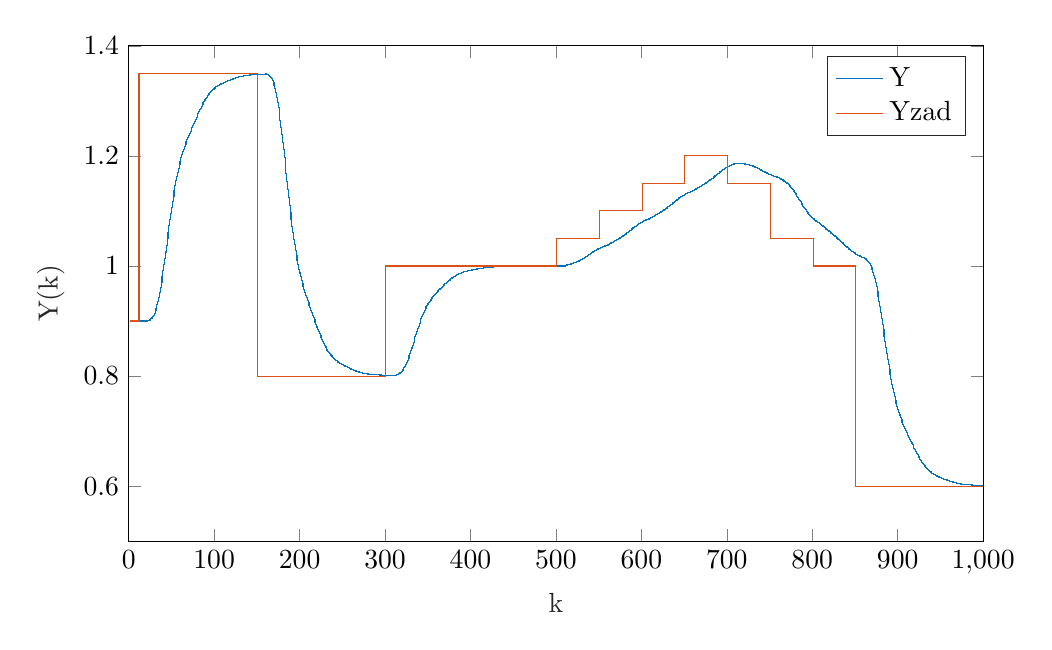
\begin{tikzpicture}

\begin{axis}[%
width=4.272in,
height=2.477in,
at={(0.717in,0.437in)},
scale only axis,
xmin=0,
xmax=1000,
xlabel style={font=\color{white!15!black}},
xlabel={k},
ymin=0.5,
ymax=1.4,
ylabel style={font=\color{white!15!black}},
ylabel={Y(k)},
axis background/.style={fill=white},
legend style={legend cell align=left, align=left, draw=white!15!black}
]
\addplot[const plot, color=mycolor1] table[row sep=crcr] {%
1	0.9\\
2	0.9\\
3	0.9\\
4	0.9\\
5	0.9\\
6	0.9\\
7	0.9\\
8	0.9\\
9	0.9\\
10	0.9\\
11	0.9\\
12	0.9\\
13	0.9\\
14	0.9\\
15	0.9\\
16	0.9\\
17	0.9\\
18	0.9\\
19	0.9\\
20	0.9\\
21	0.9\\
22	0.9003968325\\
23	0.90110505465075\\
24	0.901792976327444\\
25	0.902646481628594\\
26	0.903821675824292\\
27	0.90544848711148\\
28	0.907633879431284\\
29	0.910464715877318\\
30	0.914010308352824\\
31	0.918324685633407\\
32	0.923425663098293\\
33	0.929303840647585\\
34	0.935965438923209\\
35	0.943416013287854\\
36	0.951634745712284\\
37	0.960579528545015\\
38	0.970191311315836\\
39	0.980397805132888\\
40	0.991116627926128\\
41	1.00225796377292\\
42	1.01372812744431\\
43	1.02543354268672\\
44	1.03728153540572\\
45	1.04917966462057\\
46	1.06103743783932\\
47	1.07276903997461\\
48	1.08429539600579\\
49	1.09554568280648\\
50	1.10645838832648\\
51	1.1169820014422\\
52	1.12707532624939\\
53	1.13670736608879\\
54	1.14585695891761\\
55	1.15451243356308\\
56	1.16267122714802\\
57	1.1703392756374\\
58	1.17753016980654\\
59	1.18426415389599\\
60	1.19056702825782\\
61	1.19646900406982\\
62	1.20200355171508\\
63	1.20720628606024\\
64	1.21211392252238\\
65	1.21676331098508\\
66	1.22119054329472\\
67	1.22543014467057\\
68	1.22951436988186\\
69	1.23347262033773\\
70	1.23733099005462\\
71	1.24111194231149\\
72	1.24483411402396\\
73	1.24851224055036\\
74	1.25215718994361\\
75	1.2557760941581\\
76	1.2593725653644\\
77	1.26294698587274\\
78	1.26649685905318\\
79	1.2700172072387\\
80	1.27350100195094\\
81	1.27693961193569\\
82	1.28032325521044\\
83	1.28364144248476\\
84	1.28688340083927\\
85	1.29003846826683\\
86	1.29309645134434\\
87	1.29604793982105\\
88	1.29888457339305\\
89	1.30159925748491\\
90	1.30418632645296\\
91	1.30664165417363\\
92	1.30896271341634\\
93	1.31114858667364\\
94	1.31319993219844\\
95	1.31511890985804\\
96	1.31690907206215\\
97	1.31857522547928\\
98	1.32012326954189\\
99	1.32156001786129\\
100	1.32289300862979\\
101	1.32413030988634\\
102	1.32528032517879\\
103	1.32635160469043\\
104	1.32735266633564\\
105	1.32829183069443\\
106	1.32917707297408\\
107	1.33001589448023\\
108	1.33081521536968\\
109	1.33158128975868\\
110	1.33231964359104\\
111	1.33303503504382\\
112	1.33373143667863\\
113	1.33441203804415\\
114	1.33507926700861\\
115	1.33573482775472\\
116	1.33637975310617\\
117	1.33701446867403\\
118	1.33763886621073\\
119	1.33825238353507\\
120	1.3388540884376\\
121	1.33944276408553\\
122	1.34001699361179\\
123	1.34057524178494\\
124	1.34111593190635\\
125	1.34163751635832\\
126	1.34213853952223\\
127	1.34261769209022\\
128	1.34307385609862\\
129	1.34350614030807\\
130	1.34391390583757\\
131	1.34429678222091\\
132	1.34465467428926\\
133	1.34498776048878\\
134	1.34529648341476\\
135	1.34558153348147\\
136	1.34584382674907\\
137	1.34608447799663\\
138	1.34630477016301\\
139	1.34650612127905\\
140	1.34669004998619\\
141	1.34685814068223\\
142	1.34701200925797\\
143	1.34715327029247\\
144	1.34728350646447\\
145	1.34740424081598\\
146	1.34751691237662\\
147	1.3476228555266\\
148	1.3477232833471\\
149	1.34781927508116\\
150	1.34791176771032\\
151	1.34800155154383\\
152	1.3480892696202\\
153	1.34817542063768\\
154	1.34826036506068\\
155	1.34834433399507\\
156	1.34842744038619\\
157	1.34850969206888\\
158	1.34859100618924\\
159	1.34867122452092\\
160	1.34875012921456\\
161	1.34843062605893\\
162	1.34779790638695\\
163	1.34716201046868\\
164	1.34629858865274\\
165	1.34501935835889\\
166	1.34316774735261\\
167	1.34061500731763\\
168	1.33725674965034\\
169	1.33300986015298\\
170	1.32780975360351\\
171	1.32163087879629\\
172	1.31447733980858\\
173	1.30634095742823\\
174	1.29721934245738\\
175	1.2871417498446\\
176	1.27616294238912\\
177	1.26435794461572\\
178	1.25181757257629\\
179	1.23864463902656\\
180	1.22495074555071\\
181	1.21085225716361\\
182	1.19646593931354\\
183	1.18190777447857\\
184	1.16729311278276\\
185	1.1527343604117\\
186	1.13833773744747\\
187	1.12420083605252\\
188	1.11041083998539\\
189	1.09704328720659\\
190	1.08416127526453\\
191	1.07181510132204\\
192	1.06004237942099\\
193	1.04886844732197\\
194	1.03830679929219\\
195	1.02835961410069\\
196	1.01901856346322\\
197	1.01026589434154\\
198	1.00207569286305\\
199	0.99441525678027\\
200	0.987246519257727\\
201	0.980527475425177\\
202	0.974213563276706\\
203	0.968258961047482\\
204	0.962617790148347\\
205	0.957245223310229\\
206	0.952098482771791\\
207	0.947137703948856\\
208	0.942326646464351\\
209	0.937633244101546\\
210	0.933029992505431\\
211	0.928494179027628\\
212	0.924007963969099\\
213	0.919558326530308\\
214	0.915136890559486\\
215	0.91073964485583\\
216	0.906366572795652\\
217	0.90202120746144\\
218	0.897710129990085\\
219	0.893442429459254\\
220	0.889229142305992\\
221	0.885082688289417\\
222	0.881016318529722\\
223	0.877043589281272\\
224	0.873177873015803\\
225	0.869431916351998\\
226	0.865817452457291\\
227	0.862344873654896\\
228	0.859022968003598\\
229	0.855858721625072\\
230	0.852857186634102\\
231	0.850021412761617\\
232	0.847352439202266\\
233	0.844849341904303\\
234	0.842509330469255\\
235	0.840327888037158\\
236	0.838298946976964\\
237	0.8364150928618\\
238	0.834667789078279\\
239	0.833047614494705\\
240	0.831544506883561\\
241	0.830148005238913\\
242	0.828847484722811\\
243	0.827632378686407\\
244	0.826492383009918\\
245	0.825417638859881\\
246	0.824398890844884\\
247	0.823427618437965\\
248	0.822496139403636\\
249	0.82159768479983\\
250	0.820726445901373\\
251	0.819877594095656\\
252	0.8190472754199\\
253	0.818232581933204\\
254	0.817431502539435\\
255	0.816642856196359\\
256	0.815866210662862\\
257	0.815101790052719\\
258	0.814350374485473\\
259	0.813613195059669\\
260	0.81289182722976\\
261	0.812188085455559\\
262	0.811503921723339\\
263	0.810841330222326\\
264	0.810202260111545\\
265	0.809588537941525\\
266	0.809001800914883\\
267	0.808443441789924\\
268	0.807914565861989\\
269	0.807415960107068\\
270	0.806948074248767\\
271	0.806511013219192\\
272	0.806104540231688\\
273	0.805728089472016\\
274	0.805380787246615\\
275	0.805061480302851\\
276	0.80476876995621\\
277	0.804501050621638\\
278	0.80425655134821\\
279	0.804033378994675\\
280	0.803829561754153\\
281	0.803643091834832\\
282	0.803471966225085\\
283	0.80331422461087\\
284	0.803167983665529\\
285	0.803031467092108\\
286	0.802903030961207\\
287	0.802781184048775\\
288	0.802664603033969\\
289	0.802552142563663\\
290	0.802442840324401\\
291	0.802335917381945\\
292	0.802230774151343\\
293	0.802126982445107\\
294	0.802024274113195\\
295	0.801922526835577\\
296	0.801821747656825\\
297	0.801722054862931\\
298	0.801623658794884\\
299	0.801526842172671\\
300	0.801431940469357\\
301	0.801339322829474\\
302	0.801249373971504\\
303	0.801162477452665\\
304	0.801079000607945\\
305	0.800999281406322\\
306	0.800923617397467\\
307	0.800852256853822\\
308	0.800785392147407\\
309	0.80072315533958\\
310	0.800665615906437\\
311	0.801009432405365\\
312	0.801668802419266\\
313	0.802258407929274\\
314	0.80286868743879\\
315	0.803575929057992\\
316	0.804443966475922\\
317	0.805525694042367\\
318	0.806864419105877\\
319	0.808495067966452\\
320	0.810445260190617\\
321	0.812713329298985\\
322	0.815276397923495\\
323	0.818135464426882\\
324	0.821303566983216\\
325	0.824780441254627\\
326	0.828554991320856\\
327	0.832607407208244\\
328	0.836910973889249\\
329	0.84143361130848\\
330	0.846139180280623\\
331	0.850989911101292\\
332	0.855949432944834\\
333	0.860982601805241\\
334	0.86605354590501\\
335	0.871125901558076\\
336	0.876164268406323\\
337	0.881135331169228\\
338	0.886008704426848\\
339	0.890757548631504\\
340	0.895358998344706\\
341	0.899794360797135\\
342	0.904049000146178\\
343	0.908112074305717\\
344	0.911976408823433\\
345	0.915638471955449\\
346	0.919098255955204\\
347	0.922359021390467\\
348	0.925426944610205\\
349	0.928310700481362\\
350	0.931021005858244\\
351	0.93357014816443\\
352	0.935971529506032\\
353	0.93823925036363\\
354	0.940387730347073\\
355	0.942431350263339\\
356	0.944384113805218\\
357	0.946259340480476\\
358	0.948069400997142\\
359	0.949825501867965\\
360	0.951537522588247\\
361	0.953213905921664\\
362	0.9548615988465\\
363	0.956486038898269\\
364	0.958091179825445\\
365	0.959679551891123\\
366	0.961252353397458\\
367	0.962809569644816\\
368	0.964350114472765\\
369	0.96587198878026\\
370	0.967372450132479\\
371	0.968848187619044\\
372	0.970295496494612\\
373	0.971710447794478\\
374	0.973089048938837\\
375	0.974427392076537\\
376	0.975721787466361\\
377	0.976968879664437\\
378	0.978165744813555\\
379	0.979309967933086\\
380	0.980399699740986\\
381	0.981433693157042\\
382	0.982411320204611\\
383	0.983332570516038\\
384	0.98419803303441\\
385	0.985008862792712\\
386	0.985766734861524\\
387	0.986473787706858\\
388	0.987132558294246\\
389	0.987745911308887\\
390	0.988316964831212\\
391	0.988849014714398\\
392	0.989345459761372\\
393	0.989809729602797\\
394	0.990245216946151\\
395	0.990655215611379\\
396	0.99104286550074\\
397	0.991411105377096\\
398	0.991762634051733\\
399	0.992099880315799\\
400	0.992424981694512\\
401	0.992739771866375\\
402	0.993045776375933\\
403	0.99334421608236\\
404	0.993636017630296\\
405	0.993921830105389\\
406	0.994202046945357\\
407	0.994476832117392\\
408	0.994746149543269\\
409	0.995009794752803\\
410	0.995267427772114\\
411	0.995518606302736\\
412	0.995762818317789\\
413	0.995999513288717\\
414	0.996228131356646\\
415	0.996448129872632\\
416	0.996659006847055\\
417	0.996860320966798\\
418	0.9970517079563\\
419	0.99723289317215\\
420	0.997403700427938\\
421	0.997564057144436\\
422	0.997713996007861\\
423	0.997853653394707\\
424	0.99798326488428\\
425	0.998103158229202\\
426	0.998213744189543\\
427	0.998315505658072\\
428	0.998408985513067\\
429	0.998494773631901\\
430	0.998573493484367\\
431	0.998645788700735\\
432	0.998712309977194\\
433	0.99877370264225\\
434	0.998830595163324\\
435	0.99888358882487\\
436	0.998933248759328\\
437	0.998980096461647\\
438	0.999024603868284\\
439	0.999067189033805\\
440	0.999108213393495\\
441	0.999147980559674\\
442	0.999186736563474\\
443	0.999224671423136\\
444	0.999261921894839\\
445	0.999298575242889\\
446	0.999334673852745\\
447	0.999370220502713\\
448	0.999405184107965\\
449	0.999439505753393\\
450	0.999473104839233\\
451	0.999505885174797\\
452	0.999537740870424\\
453	0.999568561895227\\
454	0.999598239187677\\
455	0.999626669226933\\
456	0.999653757994291\\
457	0.999679424275753\\
458	0.99970360227776\\
459	0.999726243548265\\
460	0.999747318213877\\
461	0.999766815560692\\
462	0.999784744001079\\
463	0.999801130481108\\
464	0.999816019393256\\
465	0.999829471066452\\
466	0.999841559910491\\
467	0.999852372294374\\
468	0.999862004238387\\
469	0.99987055899789\\
470	0.999878144613066\\
471	0.999884871493521\\
472	0.999890850099949\\
473	0.99989618877728\\
474	0.999900991785206\\
475	0.999905357562963\\
476	0.999909377255975\\
477	0.999913133522795\\
478	0.999916699631873\\
479	0.999920138849216\\
480	0.999923504110326\\
481	0.999926837962792\\
482	0.999930172759977\\
483	0.999933531081192\\
484	0.999936926349862\\
485	0.999940363618286\\
486	0.999943840485815\\
487	0.999947348116464\\
488	0.999950872322155\\
489	0.999954394678819\\
490	0.999957893644386\\
491	0.999961345650168\\
492	0.999964726140156\\
493	0.999968010536166\\
494	0.999971175110496\\
495	0.999974197751661\\
496	0.999977058612702\\
497	0.999979740635494\\
498	0.999982229948198\\
499	0.999984516136535\\
500	0.999986592392781\\
501	0.999988455549186\\
502	0.999990106005001\\
503	0.999991547558265\\
504	0.999992787155045\\
505	0.999993834569912\\
506	0.999994702032071\\
507	0.999995403811769\\
508	0.999995955781397\\
509	0.999996374965183\\
510	0.99999667909049\\
511	1.00039371700121\\
512	1.00110205978487\\
513	1.00170452890047\\
514	1.00223442784612\\
515	1.00272038028179\\
516	1.00318686955165\\
517	1.0036547213546\\
518	1.00414153526502\\
519	1.0046620702517\\
520	1.00522858884009\\
521	1.00582821847735\\
522	1.00643043429556\\
523	1.00703349693446\\
524	1.00765531343145\\
525	1.00830831897024\\
526	1.00900037010485\\
527	1.00973551670104\\
528	1.0105146676046\\
529	1.0113361632921\\
530	1.0121962672022\\
531	1.01309091283139\\
532	1.01401816767096\\
533	1.01497748771482\\
534	1.01596699536437\\
535	1.01698282948864\\
536	1.01801983858944\\
537	1.01907214104967\\
538	1.02013357339064\\
539	1.02119804450322\\
540	1.02225981124717\\
541	1.02331361186821\\
542	1.02435455430727\\
543	1.02537791714391\\
544	1.02637915665831\\
545	1.02735409872487\\
546	1.02829911650706\\
547	1.0292112294243\\
548	1.03008814115479\\
549	1.03092823124144\\
550	1.03173051217918\\
551	1.03249456604228\\
552	1.03322048342288\\
553	1.03390882289695\\
554	1.0345605828393\\
555	1.0351771630118\\
556	1.03576030705612\\
557	1.03631203200471\\
558	1.03683455310695\\
559	1.03733021005661\\
560	1.03780139894673\\
561	1.03864646009087\\
562	1.03978062933444\\
563	1.04078845569021\\
564	1.04170584153618\\
565	1.04256377732673\\
566	1.04338885994869\\
567	1.04420376095814\\
568	1.04502765111153\\
569	1.04587658622872\\
570	1.04676385836263\\
571	1.04767742089744\\
572	1.04858747919757\\
573	1.04949291812835\\
574	1.05041206033849\\
575	1.05135752372197\\
576	1.05233715226248\\
577	1.05335482517619\\
578	1.05441115872375\\
579	1.05550411329506\\
580	1.05662951687788\\
581	1.05778283856339\\
582	1.05896166786602\\
583	1.06016497857712\\
584	1.06139042209532\\
585	1.06263369927022\\
586	1.06388927360866\\
587	1.06515094659502\\
588	1.06641231640585\\
589	1.06766713837913\\
590	1.06890960306704\\
591	1.07013446895497\\
592	1.07133694801071\\
593	1.07251250283952\\
594	1.07365684893903\\
595	1.07476614009545\\
596	1.07583713770013\\
597	1.07686729990107\\
598	1.0778548089296\\
599	1.07879855167543\\
600	1.07969806582385\\
601	1.08055346597064\\
602	1.08136537272994\\
603	1.0821348631683\\
604	1.08286343444368\\
605	1.08355295816932\\
606	1.08420561677659\\
607	1.08482382811431\\
608	1.08541016664575\\
609	1.08596728733359\\
610	1.08649785649315\\
611	1.08740029874762\\
612	1.08858979157341\\
613	1.08965096349308\\
614	1.09061989152446\\
615	1.09152769606599\\
616	1.0924010642635\\
617	1.09326272354918\\
618	1.09413187163108\\
619	1.09502456783777\\
620	1.09595408966757\\
621	1.09690837119914\\
622	1.09785761164597\\
623	1.09880070141734\\
624	1.09975596619931\\
625	1.10073602132407\\
626	1.10174870703268\\
627	1.10279790126932\\
628	1.10388422439776\\
629	1.10500564847573\\
630	1.10615802224048\\
631	1.1073368450397\\
632	1.10853974483626\\
633	1.10976573995174\\
634	1.11101253131745\\
635	1.11227587427123\\
636	1.11355029165787\\
637	1.1148296486198\\
638	1.11610761046075\\
639	1.11737800203711\\
640	1.11863508459076\\
641	1.11987368720899\\
642	1.12108909123382\\
643	1.12227682652874\\
644	1.12343267306638\\
645	1.12455284575047\\
646	1.12563416319222\\
647	1.12667413638053\\
648	1.12767099562436\\
649	1.12862367086563\\
650	1.12953173769107\\
651	1.130395343462\\
652	1.13121513656646\\
653	1.13199221710025\\
654	1.13272810082519\\
655	1.13342467390489\\
656	1.13408412968347\\
657	1.13470889373864\\
658	1.1353015455611\\
659	1.13586474293777\\
660	1.13640115330537\\
661	1.13730920133227\\
662	1.13850406499274\\
663	1.1395703725617\\
664	1.14054419953204\\
665	1.14145666520854\\
666	1.14233445634978\\
667	1.14320030092966\\
668	1.14407339829573\\
669	1.14496981062909\\
670	1.14590281955634\\
671	1.1468603645655\\
672	1.14781265145131\\
673	1.14875857826562\\
674	1.14971647939645\\
675	1.15069897987251\\
676	1.15171393046093\\
677	1.15276522028194\\
678	1.15385348133693\\
679	1.15497669759129\\
680	1.1561307297708\\
681	1.15731108911111\\
682	1.15851541519744\\
683	1.15974273756478\\
684	1.16099076781911\\
685	1.16225527131521\\
686	1.16353078015669\\
687	1.16481116791043\\
688	1.16609010741786\\
689	1.16736143015747\\
690	1.16861940307084\\
691	1.1698588600365\\
692	1.17107508631148\\
693	1.17226361484566\\
694	1.17342022792995\\
695	1.17454114208971\\
696	1.17562317694168\\
697	1.17666384395119\\
698	1.17766137346496\\
699	1.17861469511554\\
700	1.17952338392319\\
701	1.18038758651215\\
702	1.18120795044366\\
703	1.18198557497114\\
704	1.18272197506439\\
705	1.1834190362023\\
706	1.184078951199\\
707	1.18470414529443\\
708	1.18529719786099\\
709	1.18586076680438\\
710	1.18639751992523\\
711	1.18651221831475\\
712	1.18629092785924\\
713	1.18615266683395\\
714	1.18606693990674\\
715	1.18600765286384\\
716	1.18595255672064\\
717	1.18588275575563\\
718	1.18578227434336\\
719	1.18563767719582\\
720	1.18543773756889\\
721	1.18519615310595\\
722	1.18494418921743\\
723	1.1846842295491\\
724	1.18439879803255\\
725	1.18407564975217\\
726	1.18370691998225\\
727	1.18328839333299\\
728	1.18281887737155\\
729	1.18229966683755\\
730	1.18173408620468\\
731	1.18112576964288\\
732	1.18047621133567\\
733	1.17978551836803\\
734	1.17905514733567\\
735	1.17828857620041\\
736	1.17749063122264\\
737	1.17666694138931\\
738	1.17582349986878\\
739	1.17496631501848\\
740	1.17410113607155\\
741	1.1732333177918\\
742	1.17236792827358\\
743	1.17150994331535\\
744	1.17066423386293\\
745	1.16983536700897\\
746	1.16902741933029\\
747	1.16824386756392\\
748	1.16748753947557\\
749	1.16676061088764\\
750	1.16606463744184\\
751	1.16540060740034\\
752	1.16476899294972\\
753	1.16416978188346\\
754	1.16360249786905\\
755	1.16306623195307\\
756	1.16255969430794\\
757	1.16208128022535\\
758	1.16162914211492\\
759	1.16120126141339\\
760	1.16079551601878\\
761	1.16001365145738\\
762	1.15894037457367\\
763	1.15798052877069\\
764	1.15707931156364\\
765	1.15618992529156\\
766	1.15527268133295\\
767	1.15429419618655\\
768	1.1532266686384\\
769	1.15204722902929\\
770	1.15073735308466\\
771	1.1493052366589\\
772	1.14777803356319\\
773	1.14615587666895\\
774	1.14442199873985\\
775	1.14256794553579\\
776	1.14059212541136\\
777	1.13849855678803\\
778	1.1362957892123\\
779	1.13399597668459\\
780	1.13161408450484\\
781	1.12916588880959\\
782	1.12666530645259\\
783	1.12412493653425\\
784	1.12155850920695\\
785	1.11898121798116\\
786	1.11640875182568\\
787	1.11385653142127\\
788	1.11133911657954\\
789	1.10886975653239\\
790	1.10646005885781\\
791	1.10411983289513\\
792	1.10185720361568\\
793	1.09967883431872\\
794	1.09758996761927\\
795	1.09559431135825\\
796	1.09369396722249\\
797	1.0918894590782\\
798	1.09017983527501\\
799	1.08856282402788\\
800	1.08703502504983\\
801	1.08559211957906\\
802	1.08422907321397\\
803	1.08294031123552\\
804	1.08171987260122\\
805	1.08056156278147\\
806	1.07945911175469\\
807	1.0784063290746\\
808	1.07739724665759\\
809	1.07642624295296\\
810	1.07548814451595\\
811	1.07418433515173\\
812	1.07260125407848\\
813	1.07115400700819\\
814	1.06980490870859\\
815	1.06852177024251\\
816	1.06727732297586\\
817	1.06604868700549\\
818	1.06481687942964\\
819	1.06356635924957\\
820	1.06228460667134\\
821	1.06098451533583\\
822	1.05969655059005\\
823	1.05842234209261\\
824	1.05714412786465\\
825	1.05584994110756\\
826	1.05453261466811\\
827	1.05318891719762\\
828	1.05181880653853\\
829	1.05042478747156\\
830	1.04901136229311\\
831	1.04758324662967\\
832	1.04614290411372\\
833	1.04469130814368\\
834	1.04323065994807\\
835	1.04176501379597\\
836	1.04029956211728\\
837	1.03884006510026\\
838	1.03739240207448\\
839	1.03596222500649\\
840	1.03455469707677\\
841	1.03317437778697\\
842	1.03182535416059\\
843	1.0305114573318\\
844	1.02923627138778\\
845	1.02800295817699\\
846	1.02681409807654\\
847	1.02567161037729\\
848	1.02457673432857\\
849	1.02353005532998\\
850	1.02253156367392\\
851	1.02158073130043\\
852	1.02067658363713\\
853	1.01981774850737\\
854	1.01900249060918\\
855	1.01822875428551\\
856	1.01749422339825\\
857	1.01679639213189\\
858	1.01613263848402\\
859	1.01550029452341\\
860	1.0148967093382\\
861	1.01392353205634\\
862	1.01266568549135\\
863	1.01146379194913\\
864	1.01014830344722\\
865	1.00857659232235\\
866	1.00662974385191\\
867	1.00420968986861\\
868	1.00123664753952\\
869	0.997646831740664\\
870	0.993390413119296\\
871	0.988452581380834\\
872	0.982844607621753\\
873	0.9765605717512\\
874	0.969592876250273\\
875	0.961957909878341\\
876	0.953691446749461\\
877	0.944844706977621\\
878	0.935480994812871\\
879	0.925672840303994\\
880	0.915499579409624\\
881	0.90504399207581\\
882	0.894388501716754\\
883	0.883614569599948\\
884	0.872803608165325\\
885	0.862035541126998\\
886	0.851386310405085\\
887	0.840925987841813\\
888	0.83071738761177\\
889	0.820815090658765\\
890	0.811264805808438\\
891	0.802103080205753\\
892	0.793357418552412\\
893	0.785046631350171\\
894	0.777181139683411\\
895	0.769763292308008\\
896	0.762787884762076\\
897	0.756242894860035\\
898	0.750110364153481\\
899	0.744367369391171\\
900	0.738987040002324\\
901	0.733939583114274\\
902	0.729193275221195\\
903	0.724715388508976\\
904	0.720473046675956\\
905	0.716434016746523\\
906	0.712567428819872\\
907	0.708844404630999\\
908	0.705238579707156\\
909	0.701726511398523\\
910	0.698287970715558\\
911	0.694906120329759\\
912	0.691567585169746\\
913	0.68826242557543\\
914	0.684984024338255\\
915	0.681728898155307\\
916	0.678496443502662\\
917	0.675288627904062\\
918	0.672109638909076\\
919	0.66896550375867\\
920	0.665863692647641\\
921	0.662812717896865\\
922	0.659821740332846\\
923	0.65690019280369\\
924	0.654057429206078\\
925	0.651302405904297\\
926	0.648643401084628\\
927	0.646087776293423\\
928	0.643641783046377\\
929	0.641310415988031\\
930	0.639097312702113\\
931	0.63700469899082\\
932	0.635033377299871\\
933	0.633182755000572\\
934	0.631450908469906\\
935	0.629834678331045\\
936	0.628329790807601\\
937	0.626930999886161\\
938	0.625632244867703\\
939	0.624426817919554\\
940	0.623307536410482\\
941	0.622266915109787\\
942	0.621297333739002\\
943	0.62039119586067\\
944	0.619541075649477\\
945	0.618739849693879\\
946	0.617980811601001\\
947	0.617257767806917\\
948	0.616565113613426\\
949	0.615897889067111\\
950	0.615251814853368\\
951	0.614623308885504\\
952	0.614009484717019\\
953	0.613408133286624\\
954	0.612817689815588\\
955	0.612237187913612\\
956	0.611666203112794\\
957	0.611104788141406\\
958	0.610553402273809\\
959	0.610012837054638\\
960	0.609484140600628\\
961	0.6089685425389\\
962	0.608467381454282\\
963	0.607982036498353\\
964	0.607513864568163\\
965	0.607064144201329\\
966	0.606634027064722\\
967	0.606224497643939\\
968	0.605836341477269\\
969	0.605470122027138\\
970	0.605126166049681\\
971	0.604804557113496\\
972	0.604505136735531\\
973	0.604227512447966\\
974	0.603971071986485\\
975	0.603735002698274\\
976	0.60351831520709\\
977	0.603319870341987\\
978	0.603138408333929\\
979	0.602972579308368\\
980	0.602820974149068\\
981	0.602682154875911\\
982	0.602554683763622\\
983	0.602437150525799\\
984	0.602328196995612\\
985	0.602226538847511\\
986	0.602130984019804\\
987	0.602040447612789\\
988	0.601953963148308\\
989	0.601870690181603\\
990	0.601789918352816\\
991	0.601711068051767\\
992	0.601633687944194\\
993	0.601557449669557\\
994	0.601482140069199\\
995	0.601407651338948\\
996	0.601333969522305\\
997	0.601261161769759\\
998	0.601189362787216\\
999	0.601118760883205\\
1000	0.601049584001516\\
};
\addlegendentry{Y}

\addplot[const plot, color=mycolor2] table[row sep=crcr] {%
1	0.9\\
2	0.9\\
3	0.9\\
4	0.9\\
5	0.9\\
6	0.9\\
7	0.9\\
8	0.9\\
9	0.9\\
10	0.9\\
11	0.9\\
12	1.35\\
13	1.35\\
14	1.35\\
15	1.35\\
16	1.35\\
17	1.35\\
18	1.35\\
19	1.35\\
20	1.35\\
21	1.35\\
22	1.35\\
23	1.35\\
24	1.35\\
25	1.35\\
26	1.35\\
27	1.35\\
28	1.35\\
29	1.35\\
30	1.35\\
31	1.35\\
32	1.35\\
33	1.35\\
34	1.35\\
35	1.35\\
36	1.35\\
37	1.35\\
38	1.35\\
39	1.35\\
40	1.35\\
41	1.35\\
42	1.35\\
43	1.35\\
44	1.35\\
45	1.35\\
46	1.35\\
47	1.35\\
48	1.35\\
49	1.35\\
50	1.35\\
51	1.35\\
52	1.35\\
53	1.35\\
54	1.35\\
55	1.35\\
56	1.35\\
57	1.35\\
58	1.35\\
59	1.35\\
60	1.35\\
61	1.35\\
62	1.35\\
63	1.35\\
64	1.35\\
65	1.35\\
66	1.35\\
67	1.35\\
68	1.35\\
69	1.35\\
70	1.35\\
71	1.35\\
72	1.35\\
73	1.35\\
74	1.35\\
75	1.35\\
76	1.35\\
77	1.35\\
78	1.35\\
79	1.35\\
80	1.35\\
81	1.35\\
82	1.35\\
83	1.35\\
84	1.35\\
85	1.35\\
86	1.35\\
87	1.35\\
88	1.35\\
89	1.35\\
90	1.35\\
91	1.35\\
92	1.35\\
93	1.35\\
94	1.35\\
95	1.35\\
96	1.35\\
97	1.35\\
98	1.35\\
99	1.35\\
100	1.35\\
101	1.35\\
102	1.35\\
103	1.35\\
104	1.35\\
105	1.35\\
106	1.35\\
107	1.35\\
108	1.35\\
109	1.35\\
110	1.35\\
111	1.35\\
112	1.35\\
113	1.35\\
114	1.35\\
115	1.35\\
116	1.35\\
117	1.35\\
118	1.35\\
119	1.35\\
120	1.35\\
121	1.35\\
122	1.35\\
123	1.35\\
124	1.35\\
125	1.35\\
126	1.35\\
127	1.35\\
128	1.35\\
129	1.35\\
130	1.35\\
131	1.35\\
132	1.35\\
133	1.35\\
134	1.35\\
135	1.35\\
136	1.35\\
137	1.35\\
138	1.35\\
139	1.35\\
140	1.35\\
141	1.35\\
142	1.35\\
143	1.35\\
144	1.35\\
145	1.35\\
146	1.35\\
147	1.35\\
148	1.35\\
149	1.35\\
150	1.35\\
151	0.8\\
152	0.8\\
153	0.8\\
154	0.8\\
155	0.8\\
156	0.8\\
157	0.8\\
158	0.8\\
159	0.8\\
160	0.8\\
161	0.8\\
162	0.8\\
163	0.8\\
164	0.8\\
165	0.8\\
166	0.8\\
167	0.8\\
168	0.8\\
169	0.8\\
170	0.8\\
171	0.8\\
172	0.8\\
173	0.8\\
174	0.8\\
175	0.8\\
176	0.8\\
177	0.8\\
178	0.8\\
179	0.8\\
180	0.8\\
181	0.8\\
182	0.8\\
183	0.8\\
184	0.8\\
185	0.8\\
186	0.8\\
187	0.8\\
188	0.8\\
189	0.8\\
190	0.8\\
191	0.8\\
192	0.8\\
193	0.8\\
194	0.8\\
195	0.8\\
196	0.8\\
197	0.8\\
198	0.8\\
199	0.8\\
200	0.8\\
201	0.8\\
202	0.8\\
203	0.8\\
204	0.8\\
205	0.8\\
206	0.8\\
207	0.8\\
208	0.8\\
209	0.8\\
210	0.8\\
211	0.8\\
212	0.8\\
213	0.8\\
214	0.8\\
215	0.8\\
216	0.8\\
217	0.8\\
218	0.8\\
219	0.8\\
220	0.8\\
221	0.8\\
222	0.8\\
223	0.8\\
224	0.8\\
225	0.8\\
226	0.8\\
227	0.8\\
228	0.8\\
229	0.8\\
230	0.8\\
231	0.8\\
232	0.8\\
233	0.8\\
234	0.8\\
235	0.8\\
236	0.8\\
237	0.8\\
238	0.8\\
239	0.8\\
240	0.8\\
241	0.8\\
242	0.8\\
243	0.8\\
244	0.8\\
245	0.8\\
246	0.8\\
247	0.8\\
248	0.8\\
249	0.8\\
250	0.8\\
251	0.8\\
252	0.8\\
253	0.8\\
254	0.8\\
255	0.8\\
256	0.8\\
257	0.8\\
258	0.8\\
259	0.8\\
260	0.8\\
261	0.8\\
262	0.8\\
263	0.8\\
264	0.8\\
265	0.8\\
266	0.8\\
267	0.8\\
268	0.8\\
269	0.8\\
270	0.8\\
271	0.8\\
272	0.8\\
273	0.8\\
274	0.8\\
275	0.8\\
276	0.8\\
277	0.8\\
278	0.8\\
279	0.8\\
280	0.8\\
281	0.8\\
282	0.8\\
283	0.8\\
284	0.8\\
285	0.8\\
286	0.8\\
287	0.8\\
288	0.8\\
289	0.8\\
290	0.8\\
291	0.8\\
292	0.8\\
293	0.8\\
294	0.8\\
295	0.8\\
296	0.8\\
297	0.8\\
298	0.8\\
299	0.8\\
300	0.8\\
301	1\\
302	1\\
303	1\\
304	1\\
305	1\\
306	1\\
307	1\\
308	1\\
309	1\\
310	1\\
311	1\\
312	1\\
313	1\\
314	1\\
315	1\\
316	1\\
317	1\\
318	1\\
319	1\\
320	1\\
321	1\\
322	1\\
323	1\\
324	1\\
325	1\\
326	1\\
327	1\\
328	1\\
329	1\\
330	1\\
331	1\\
332	1\\
333	1\\
334	1\\
335	1\\
336	1\\
337	1\\
338	1\\
339	1\\
340	1\\
341	1\\
342	1\\
343	1\\
344	1\\
345	1\\
346	1\\
347	1\\
348	1\\
349	1\\
350	1\\
351	1\\
352	1\\
353	1\\
354	1\\
355	1\\
356	1\\
357	1\\
358	1\\
359	1\\
360	1\\
361	1\\
362	1\\
363	1\\
364	1\\
365	1\\
366	1\\
367	1\\
368	1\\
369	1\\
370	1\\
371	1\\
372	1\\
373	1\\
374	1\\
375	1\\
376	1\\
377	1\\
378	1\\
379	1\\
380	1\\
381	1\\
382	1\\
383	1\\
384	1\\
385	1\\
386	1\\
387	1\\
388	1\\
389	1\\
390	1\\
391	1\\
392	1\\
393	1\\
394	1\\
395	1\\
396	1\\
397	1\\
398	1\\
399	1\\
400	1\\
401	1\\
402	1\\
403	1\\
404	1\\
405	1\\
406	1\\
407	1\\
408	1\\
409	1\\
410	1\\
411	1\\
412	1\\
413	1\\
414	1\\
415	1\\
416	1\\
417	1\\
418	1\\
419	1\\
420	1\\
421	1\\
422	1\\
423	1\\
424	1\\
425	1\\
426	1\\
427	1\\
428	1\\
429	1\\
430	1\\
431	1\\
432	1\\
433	1\\
434	1\\
435	1\\
436	1\\
437	1\\
438	1\\
439	1\\
440	1\\
441	1\\
442	1\\
443	1\\
444	1\\
445	1\\
446	1\\
447	1\\
448	1\\
449	1\\
450	1\\
451	1\\
452	1\\
453	1\\
454	1\\
455	1\\
456	1\\
457	1\\
458	1\\
459	1\\
460	1\\
461	1\\
462	1\\
463	1\\
464	1\\
465	1\\
466	1\\
467	1\\
468	1\\
469	1\\
470	1\\
471	1\\
472	1\\
473	1\\
474	1\\
475	1\\
476	1\\
477	1\\
478	1\\
479	1\\
480	1\\
481	1\\
482	1\\
483	1\\
484	1\\
485	1\\
486	1\\
487	1\\
488	1\\
489	1\\
490	1\\
491	1\\
492	1\\
493	1\\
494	1\\
495	1\\
496	1\\
497	1\\
498	1\\
499	1\\
500	1\\
501	1.05\\
502	1.05\\
503	1.05\\
504	1.05\\
505	1.05\\
506	1.05\\
507	1.05\\
508	1.05\\
509	1.05\\
510	1.05\\
511	1.05\\
512	1.05\\
513	1.05\\
514	1.05\\
515	1.05\\
516	1.05\\
517	1.05\\
518	1.05\\
519	1.05\\
520	1.05\\
521	1.05\\
522	1.05\\
523	1.05\\
524	1.05\\
525	1.05\\
526	1.05\\
527	1.05\\
528	1.05\\
529	1.05\\
530	1.05\\
531	1.05\\
532	1.05\\
533	1.05\\
534	1.05\\
535	1.05\\
536	1.05\\
537	1.05\\
538	1.05\\
539	1.05\\
540	1.05\\
541	1.05\\
542	1.05\\
543	1.05\\
544	1.05\\
545	1.05\\
546	1.05\\
547	1.05\\
548	1.05\\
549	1.05\\
550	1.05\\
551	1.1\\
552	1.1\\
553	1.1\\
554	1.1\\
555	1.1\\
556	1.1\\
557	1.1\\
558	1.1\\
559	1.1\\
560	1.1\\
561	1.1\\
562	1.1\\
563	1.1\\
564	1.1\\
565	1.1\\
566	1.1\\
567	1.1\\
568	1.1\\
569	1.1\\
570	1.1\\
571	1.1\\
572	1.1\\
573	1.1\\
574	1.1\\
575	1.1\\
576	1.1\\
577	1.1\\
578	1.1\\
579	1.1\\
580	1.1\\
581	1.1\\
582	1.1\\
583	1.1\\
584	1.1\\
585	1.1\\
586	1.1\\
587	1.1\\
588	1.1\\
589	1.1\\
590	1.1\\
591	1.1\\
592	1.1\\
593	1.1\\
594	1.1\\
595	1.1\\
596	1.1\\
597	1.1\\
598	1.1\\
599	1.1\\
600	1.1\\
601	1.15\\
602	1.15\\
603	1.15\\
604	1.15\\
605	1.15\\
606	1.15\\
607	1.15\\
608	1.15\\
609	1.15\\
610	1.15\\
611	1.15\\
612	1.15\\
613	1.15\\
614	1.15\\
615	1.15\\
616	1.15\\
617	1.15\\
618	1.15\\
619	1.15\\
620	1.15\\
621	1.15\\
622	1.15\\
623	1.15\\
624	1.15\\
625	1.15\\
626	1.15\\
627	1.15\\
628	1.15\\
629	1.15\\
630	1.15\\
631	1.15\\
632	1.15\\
633	1.15\\
634	1.15\\
635	1.15\\
636	1.15\\
637	1.15\\
638	1.15\\
639	1.15\\
640	1.15\\
641	1.15\\
642	1.15\\
643	1.15\\
644	1.15\\
645	1.15\\
646	1.15\\
647	1.15\\
648	1.15\\
649	1.15\\
650	1.15\\
651	1.2\\
652	1.2\\
653	1.2\\
654	1.2\\
655	1.2\\
656	1.2\\
657	1.2\\
658	1.2\\
659	1.2\\
660	1.2\\
661	1.2\\
662	1.2\\
663	1.2\\
664	1.2\\
665	1.2\\
666	1.2\\
667	1.2\\
668	1.2\\
669	1.2\\
670	1.2\\
671	1.2\\
672	1.2\\
673	1.2\\
674	1.2\\
675	1.2\\
676	1.2\\
677	1.2\\
678	1.2\\
679	1.2\\
680	1.2\\
681	1.2\\
682	1.2\\
683	1.2\\
684	1.2\\
685	1.2\\
686	1.2\\
687	1.2\\
688	1.2\\
689	1.2\\
690	1.2\\
691	1.2\\
692	1.2\\
693	1.2\\
694	1.2\\
695	1.2\\
696	1.2\\
697	1.2\\
698	1.2\\
699	1.2\\
700	1.2\\
701	1.15\\
702	1.15\\
703	1.15\\
704	1.15\\
705	1.15\\
706	1.15\\
707	1.15\\
708	1.15\\
709	1.15\\
710	1.15\\
711	1.15\\
712	1.15\\
713	1.15\\
714	1.15\\
715	1.15\\
716	1.15\\
717	1.15\\
718	1.15\\
719	1.15\\
720	1.15\\
721	1.15\\
722	1.15\\
723	1.15\\
724	1.15\\
725	1.15\\
726	1.15\\
727	1.15\\
728	1.15\\
729	1.15\\
730	1.15\\
731	1.15\\
732	1.15\\
733	1.15\\
734	1.15\\
735	1.15\\
736	1.15\\
737	1.15\\
738	1.15\\
739	1.15\\
740	1.15\\
741	1.15\\
742	1.15\\
743	1.15\\
744	1.15\\
745	1.15\\
746	1.15\\
747	1.15\\
748	1.15\\
749	1.15\\
750	1.15\\
751	1.05\\
752	1.05\\
753	1.05\\
754	1.05\\
755	1.05\\
756	1.05\\
757	1.05\\
758	1.05\\
759	1.05\\
760	1.05\\
761	1.05\\
762	1.05\\
763	1.05\\
764	1.05\\
765	1.05\\
766	1.05\\
767	1.05\\
768	1.05\\
769	1.05\\
770	1.05\\
771	1.05\\
772	1.05\\
773	1.05\\
774	1.05\\
775	1.05\\
776	1.05\\
777	1.05\\
778	1.05\\
779	1.05\\
780	1.05\\
781	1.05\\
782	1.05\\
783	1.05\\
784	1.05\\
785	1.05\\
786	1.05\\
787	1.05\\
788	1.05\\
789	1.05\\
790	1.05\\
791	1.05\\
792	1.05\\
793	1.05\\
794	1.05\\
795	1.05\\
796	1.05\\
797	1.05\\
798	1.05\\
799	1.05\\
800	1.05\\
801	1\\
802	1\\
803	1\\
804	1\\
805	1\\
806	1\\
807	1\\
808	1\\
809	1\\
810	1\\
811	1\\
812	1\\
813	1\\
814	1\\
815	1\\
816	1\\
817	1\\
818	1\\
819	1\\
820	1\\
821	1\\
822	1\\
823	1\\
824	1\\
825	1\\
826	1\\
827	1\\
828	1\\
829	1\\
830	1\\
831	1\\
832	1\\
833	1\\
834	1\\
835	1\\
836	1\\
837	1\\
838	1\\
839	1\\
840	1\\
841	1\\
842	1\\
843	1\\
844	1\\
845	1\\
846	1\\
847	1\\
848	1\\
849	1\\
850	1\\
851	0.6\\
852	0.6\\
853	0.6\\
854	0.6\\
855	0.6\\
856	0.6\\
857	0.6\\
858	0.6\\
859	0.6\\
860	0.6\\
861	0.6\\
862	0.6\\
863	0.6\\
864	0.6\\
865	0.6\\
866	0.6\\
867	0.6\\
868	0.6\\
869	0.6\\
870	0.6\\
871	0.6\\
872	0.6\\
873	0.6\\
874	0.6\\
875	0.6\\
876	0.6\\
877	0.6\\
878	0.6\\
879	0.6\\
880	0.6\\
881	0.6\\
882	0.6\\
883	0.6\\
884	0.6\\
885	0.6\\
886	0.6\\
887	0.6\\
888	0.6\\
889	0.6\\
890	0.6\\
891	0.6\\
892	0.6\\
893	0.6\\
894	0.6\\
895	0.6\\
896	0.6\\
897	0.6\\
898	0.6\\
899	0.6\\
900	0.6\\
901	0.6\\
902	0.6\\
903	0.6\\
904	0.6\\
905	0.6\\
906	0.6\\
907	0.6\\
908	0.6\\
909	0.6\\
910	0.6\\
911	0.6\\
912	0.6\\
913	0.6\\
914	0.6\\
915	0.6\\
916	0.6\\
917	0.6\\
918	0.6\\
919	0.6\\
920	0.6\\
921	0.6\\
922	0.6\\
923	0.6\\
924	0.6\\
925	0.6\\
926	0.6\\
927	0.6\\
928	0.6\\
929	0.6\\
930	0.6\\
931	0.6\\
932	0.6\\
933	0.6\\
934	0.6\\
935	0.6\\
936	0.6\\
937	0.6\\
938	0.6\\
939	0.6\\
940	0.6\\
941	0.6\\
942	0.6\\
943	0.6\\
944	0.6\\
945	0.6\\
946	0.6\\
947	0.6\\
948	0.6\\
949	0.6\\
950	0.6\\
951	0.6\\
952	0.6\\
953	0.6\\
954	0.6\\
955	0.6\\
956	0.6\\
957	0.6\\
958	0.6\\
959	0.6\\
960	0.6\\
961	0.6\\
962	0.6\\
963	0.6\\
964	0.6\\
965	0.6\\
966	0.6\\
967	0.6\\
968	0.6\\
969	0.6\\
970	0.6\\
971	0.6\\
972	0.6\\
973	0.6\\
974	0.6\\
975	0.6\\
976	0.6\\
977	0.6\\
978	0.6\\
979	0.6\\
980	0.6\\
981	0.6\\
982	0.6\\
983	0.6\\
984	0.6\\
985	0.6\\
986	0.6\\
987	0.6\\
988	0.6\\
989	0.6\\
990	0.6\\
991	0.6\\
992	0.6\\
993	0.6\\
994	0.6\\
995	0.6\\
996	0.6\\
997	0.6\\
998	0.6\\
999	0.6\\
1000	0.6\\
};
\addlegendentry{Yzad}

\end{axis}
\end{tikzpicture}%
\caption{Śledzenie wartości zadanej dla parametrów $K = 1,212$, $T_i = 15$, $T_d = 4$}
\end{figure}

Wskaźnik jakości regulacji:

\begin{equation}
E = 25,6710
\end{equation}

Wartości parametrów dla których wartość wyjścia najlepiej śledzi wartość zadaną (na oko) to:

\begin{equation}
K = 1,3; T_i = 10; T_d = 3;
\end{equation}

\begin{figure}[H]
\centering
% This file was created by matlab2tikz.
%
%The latest updates can be retrieved from
%  http://www.mathworks.com/matlabcentral/fileexchange/22022-matlab2tikz-matlab2tikz
%where you can also make suggestions and rate matlab2tikz.
%
\definecolor{mycolor1}{rgb}{0.00000,0.44700,0.74100}%
%
\begin{tikzpicture}

\begin{axis}[%
width=4.272in,
height=2.477in,
at={(0.717in,0.437in)},
scale only axis,
xmin=0,
xmax=1000,
xlabel style={font=\color{white!15!black}},
xlabel={k},
ymin=2.7,
ymax=3.3,
ylabel style={font=\color{white!15!black}},
ylabel={U(k)},
axis background/.style={fill=white}
]
\addplot[const plot, color=mycolor1, forget plot] table[row sep=crcr] {%
1	3\\
2	3\\
3	3\\
4	3\\
5	3\\
6	3\\
7	3\\
8	3\\
9	3\\
10	3\\
11	3\\
12	3.075\\
13	3\\
14	3.02925\\
15	3.0585\\
16	3.08775\\
17	3.117\\
18	3.14625\\
19	3.1755\\
20	3.20475\\
21	3.234\\
22	3.25962592719375\\
23	3.28547758778953\\
24	3.3\\
25	3.3\\
26	3.3\\
27	3.3\\
28	3.3\\
29	3.3\\
30	3.3\\
31	3.3\\
32	3.3\\
33	3.3\\
34	3.3\\
35	3.3\\
36	3.3\\
37	3.3\\
38	3.3\\
39	3.3\\
40	3.3\\
41	3.3\\
42	3.3\\
43	3.3\\
44	3.3\\
45	3.3\\
46	3.3\\
47	3.3\\
48	3.3\\
49	3.3\\
50	3.3\\
51	3.3\\
52	3.3\\
53	3.29999906788716\\
54	3.29989615394184\\
55	3.29969413415641\\
56	3.29939607445979\\
57	3.29900518175031\\
58	3.29852476159182\\
59	3.29795818181419\\
60	3.29730884133915\\
61	3.29658014362351\\
62	3.2957754741763\\
63	3.29489822670512\\
64	3.2939566673918\\
65	3.29296343597744\\
66	3.29193075207795\\
67	3.29087041086821\\
68	3.28979378207084\\
69	3.28871181170071\\
70	3.28763502609109\\
71	3.28657353779293\\
72	3.28553705299544\\
73	3.28453487799008\\
74	3.28357568874757\\
75	3.28266710362615\\
76	3.28181551294273\\
77	3.28102612746637\\
78	3.28030302497752\\
79	3.27964919493\\
80	3.27906658126531\\
81	3.27855612343809\\
82	3.27811779571788\\
83	3.27775064494117\\
84	3.27745283837678\\
85	3.27722174210043\\
86	3.27705402636426\\
87	3.27694577561768\\
88	3.27689259344666\\
89	3.27688970284671\\
90	3.27693204220213\\
91	3.27701435730552\\
92	3.27713128971614\\
93	3.27727746171895\\
94	3.27744755755259\\
95	3.27763639904149\\
96	3.2778390130042\\
97	3.27805068905315\\
98	3.2782670278833\\
99	3.27848398055016\\
100	3.27869787917931\\
101	3.27890545949888\\
102	3.27910387554193\\
103	3.27929070682806\\
104	3.27946395832833\\
105	3.27962205361544\\
106	3.27976382180672\\
107	3.27988847908774\\
108	3.27999560565695\\
109	3.28008511889793\\
110	3.28015724353904\\
111	3.2802124795202\\
112	3.28025156825236\\
113	3.28027545792607\\
114	3.2802852684994\\
115	3.28028225696565\\
116	3.28026778345733\\
117	3.28024327868175\\
118	3.28021021311212\\
119	3.28017006828628\\
120	3.28012431049755\\
121	3.28007436709875\\
122	3.28002160558078\\
123	3.27996731552982\\
124	3.27991269351272\\
125	3.2798588308879\\
126	3.27980670448984\\
127	3.27975717009078\\
128	3.27971095850442\\
129	3.27966867416406\\
130	3.27963079598116\\
131	3.2795976802692\\
132	3.27956956550261\\
133	3.27954657866953\\
134	3.27952874297145\\
135	3.27951598662136\\
136	3.27950815249504\\
137	3.27950500839691\\
138	3.27950625771235\\
139	3.27951155023166\\
140	3.27952049294683\\
141	3.27953266063978\\
142	3.2795476061003\\
143	3.2795648698318\\
144	3.27958398912433\\
145	3.27960450639507\\
146	3.27962597671786\\
147	3.27964797448368\\
148	3.27967009915378\\
149	3.27969198008599\\
150	3.279713280432\\
151	3.204713280432\\
152	3.279713280432\\
153	3.24398119531552\\
154	3.20824756674577\\
155	3.17251225450489\\
156	3.13677515772019\\
157	3.10103621332434\\
158	3.06529539399956\\
159	3.02955270568525\\
160	2.99380818472878\\
161	2.96168695426391\\
162	2.92934016572859\\
163	2.8952734647236\\
164	2.8645656615514\\
165	2.83719207628773\\
166	2.81313444750751\\
167	2.79238005668261\\
168	2.77492095208089\\
169	2.7607532618056\\
170	2.74987658664479\\
171	2.74211829793672\\
172	2.73732996063767\\
173	2.73561413989766\\
174	2.73689662253244\\
175	2.74087402965821\\
176	2.74724811725953\\
177	2.75572439904582\\
178	2.76601096397938\\
179	2.77781746497988\\
180	2.7908542579651\\
181	2.80484013696361\\
182	2.81950860756262\\
183	2.83459424736055\\
184	2.84982955641432\\
185	2.86496395010145\\
186	2.87977370408541\\
187	2.89406124465062\\
188	2.90765463892406\\
189	2.92040725560769\\
190	2.93219757060098\\
191	2.9429286861945\\
192	2.95252723709803\\
193	2.96094271043784\\
194	2.9681475722768\\
195	2.97413663949405\\
196	2.97892512506239\\
197	2.98254629097426\\
198	2.98504918259913\\
199	2.98649642002157\\
200	2.9869620256497\\
201	2.98652929038304\\
202	2.98528871680607\\
203	2.98333604350024\\
204	2.98077028927413\\
205	2.97769181467166\\
206	2.97420049750389\\
207	2.97039409972362\\
208	2.96636683726382\\
209	2.96220814448397\\
210	2.9580016275838\\
211	2.95382420267113\\
212	2.94974541261903\\
213	2.94582691525464\\
214	2.9421221385113\\
215	2.93867610133961\\
216	2.93552539479219\\
217	2.93269830971696\\
218	2.93021509360259\\
219	2.92808831917948\\
220	2.92632334817118\\
221	2.92491887414612\\
222	2.92386752894845\\
223	2.92315653782996\\
224	2.92276840894212\\
225	2.92268164306659\\
226	2.92287144973165\\
227	2.92331045670227\\
228	2.92396940120878\\
229	2.92481779281356\\
230	2.92582453929555\\
231	2.92695852833971\\
232	2.92818915916978\\
233	2.92948681955584\\
234	2.93082330486692\\
235	2.93217217704446\\
236	2.93350906256003\\
237	2.93481188956012\\
238	2.93606106544315\\
239	2.93723959702664\\
240	2.93833315624342\\
241	2.93933009496195\\
242	2.94022141306311\\
243	2.94100068433087\\
244	2.94166394503144\\
245	2.94220955026974\\
246	2.94263800332421\\
247	2.94295176317534\\
248	2.94315503536418\\
249	2.94325355115678\\
250	2.94325433975836\\
251	2.94316549802989\\
252	2.94299596181925\\
253	2.94275528263926\\
254	2.94245341301512\\
255	2.94210050339325\\
256	2.94170671306028\\
257	2.94128203707407\\
258	2.94083615076609\\
259	2.94037827294323\\
260	2.93991704850421\\
261	2.93946045079626\\
262	2.93901570367611\\
263	2.93858922290926\\
264	2.93818657624609\\
265	2.93781246125401\\
266	2.93747069976339\\
267	2.93716424760175\\
268	2.9368952181457\\
269	2.93666491811189\\
270	2.93647389393676\\
271	2.93632198705672\\
272	2.93620839639428\\
273	2.93613174637888\\
274	2.93609015888021\\
275	2.93608132750444\\
276	2.93610259279623\\
277	2.9361510169985\\
278	2.9362234571447\\
279	2.93631663539095\\
280	2.93642720563573\\
281	2.93655181561836\\
282	2.93668716383358\\
283	2.93683005074301\\
284	2.93697742390559\\
285	2.9371264167836\\
286	2.9372743811087\\
287	2.93741891281093\\
288	2.93755787162226\\
289	2.9376893945632\\
290	2.93781190360694\\
291	2.93792410788819\\
292	2.93802500088495\\
293	2.9381138530497\\
294	2.93819020040247\\
295	2.93825382962286\\
296	2.93830476019126\\
297	2.93834322413233\\
298	2.93836964390695\\
299	2.93838460898374\\
300	2.93838885159786\\
301	3.01338885159786\\
302	2.93838885159786\\
303	2.95136638032129\\
304	2.96433705568201\\
305	2.97730196307516\\
306	2.99026219224518\\
307	3.0032188185203\\
308	3.01617288589561\\
309	3.02912539209232\\
310	3.04207727567605\\
311	3.0514050604503\\
312	3.0609586561571\\
313	3.07333183824591\\
314	3.08447715169318\\
315	3.0944052788983\\
316	3.10312434884923\\
317	3.11064026866244\\
318	3.11695701914318\\
319	3.12207691811333\\
320	3.12600085485576\\
321	3.12890363052781\\
322	3.13093724181877\\
323	3.13195077161946\\
324	3.13187146399642\\
325	3.13081121944737\\
326	3.12887977544918\\
327	3.12618524548746\\
328	3.12283458378199\\
329	3.11893398450637\\
330	3.11458922330713\\
331	3.10989748550455\\
332	3.10494072870328\\
333	3.09980158402992\\
334	3.09457347125021\\
335	3.08934806661633\\
336	3.08420704162948\\
337	3.07922236230775\\
338	3.07445651024709\\
339	3.06996263676065\\
340	3.06578465995624\\
341	3.06195772227656\\
342	3.05850932315462\\
343	3.0554599653383\\
344	3.05282257250837\\
345	3.05060204921352\\
346	3.04879581038139\\
347	3.04739466422155\\
348	3.04638366046292\\
349	3.04574291352426\\
350	3.04544840877026\\
351	3.04547277899342\\
352	3.04578600380786\\
353	3.04635602648835\\
354	3.047149371439\\
355	3.04813181218646\\
356	3.04926903667085\\
357	3.0505272490004\\
358	3.05187369411603\\
359	3.05327710897594\\
360	3.05470810279951\\
361	3.05613946896147\\
362	3.05754643383201\\
363	3.05890685011858\\
364	3.06020133833962\\
365	3.06141337375284\\
366	3.06252931632448\\
367	3.06353838667122\\
368	3.06443259427652\\
369	3.06520662465066\\
370	3.06585769175482\\
371	3.06638536172648\\
372	3.06679135354417\\
373	3.06707932165211\\
374	3.06725462504869\\
375	3.06732408732115\\
376	3.06729575236777\\
377	3.06717864053892\\
378	3.06698250951579\\
379	3.06671762366658\\
380	3.06639453504785\\
381	3.06602387868025\\
382	3.06561618422433\\
383	3.06518170572878\\
384	3.06473027072234\\
385	3.06427114954431\\
386	3.06381294541834\\
387	3.06336350537096\\
388	3.06292985171175\\
389	3.0625181334511\\
390	3.0621335967425\\
391	3.06178057319517\\
392	3.06146248470769\\
393	3.06118186331825\\
394	3.06094038444894\\
395	3.06073891183549\\
396	3.06057755237999\\
397	3.06045571914435\\
398	3.0603722007154\\
399	3.06032523521703\\
400	3.06031258731528\\
401	3.06033162665511\\
402	3.06037940627856\\
403	3.06045273969878\\
404	3.0605482754408\\
405	3.06066256800394\\
406	3.06079214435047\\
407	3.06093356517743\\
408	3.06108348038058\\
409	3.0612386782685\\
410	3.06139612822864\\
411	3.06155301668362\\
412	3.06170677630313\\
413	3.0618551085539\\
414	3.06199599977561\\
415	3.06212773106406\\
416	3.06224888232354\\
417	3.06235833091794\\
418	3.06245524540496\\
419	3.06253907487921\\
420	3.06260953447964\\
421	3.06266658763368\\
422	3.0627104256171\\
423	3.06274144500405\\
424	3.06276022356874\\
425	3.06276749517806\\
426	3.06276412418559\\
427	3.06275107980227\\
428	3.0627294108788\\
429	3.0627002214905\\
430	3.06266464766891\\
431	3.06262383557499\\
432	3.06257892135989\\
433	3.06253101290915\\
434	3.06248117361819\\
435	3.06243040829959\\
436	3.0623796512783\\
437	3.0623297566892\\
438	3.06228149095275\\
439	3.06223552737017\\
440	3.06219244274833\\
441	3.06215271593842\\
442	3.0621167281495\\
443	3.0620847648806\\
444	3.06205701930032\\
445	3.06203359689365\\
446	3.06201452118949\\
447	3.0619997403799\\
448	3.06198913464348\\
449	3.06198252398919\\
450	3.06197967644393\\
451	3.06198031641643\\
452	3.06198413308134\\
453	3.06199078864049\\
454	3.0619999263323\\
455	3.06201117807602\\
456	3.06202417165285\\
457	3.06203853734257\\
458	3.0620539139502\\
459	3.06206995417309\\
460	3.06208632927452\\
461	3.06210273304393\\
462	3.06211888503829\\
463	3.06213453311111\\
464	3.0621494552475\\
465	3.06216346073362\\
466	3.06217639069763\\
467	3.06218811806688\\
468	3.06219854699187\\
469	3.06220761179245\\
470	3.06221527548468\\
471	3.06222152794934\\
472	3.06222638380343\\
473	3.06222988003619\\
474	3.06223207346946\\
475	3.06223303810049\\
476	3.06223286238197\\
477	3.06223164649066\\
478	3.0622294996316\\
479	3.06222653742049\\
480	3.0622228793817\\
481	3.06221864659421\\
482	3.06221395951263\\
483	3.06220893598521\\
484	3.06220368948522\\
485	3.06219832756761\\
486	3.06219295055746\\
487	3.06218765047282\\
488	3.06218251017986\\
489	3.06217760277486\\
490	3.06217299118408\\
491	3.06216872796956\\
492	3.06216485532659\\
493	3.06216140525652\\
494	3.06215839989688\\
495	3.06215585199002\\
496	3.06215376547022\\
497	3.06215213614951\\
498	3.06215095248195\\
499	3.06215019638696\\
500	3.06214984411257\\
501	3.13714984411257\\
502	3.06214984411257\\
503	3.06540051736922\\
504	3.06865146041689\\
505	3.07190263430655\\
506	3.07515399952075\\
507	3.0784055166891\\
508	3.08165714724024\\
509	3.08490885398453\\
510	3.08816060162372\\
511	3.08778828549059\\
512	3.08764169911338\\
513	3.09078471061612\\
514	3.09361032516374\\
515	3.09612240179603\\
516	3.09832403485554\\
517	3.10021765274573\\
518	3.10180510565805\\
519	3.10308774340715\\
520	3.10406648440206\\
521	3.10491699534205\\
522	3.10579281026965\\
523	3.10652236827626\\
524	3.10697011961753\\
525	3.10716619676496\\
526	3.10713990529602\\
527	3.10691989240234\\
528	3.10653429277736\\
529	3.10601085456495\\
530	3.1053770477505\\
531	3.10465169520409\\
532	3.10383817140328\\
533	3.10294126719137\\
534	3.10198028240997\\
535	3.10097925332008\\
536	3.09995940607793\\
537	3.09893927546674\\
538	3.0979347985322\\
539	3.09695938663515\\
540	3.09602397899335\\
541	3.09513748928303\\
542	3.09430795465323\\
543	3.09354316795145\\
544	3.09284990086502\\
545	3.09223300768589\\
546	3.09169534633163\\
547	3.09123803654083\\
548	3.09086070378409\\
549	3.09056171204323\\
550	3.09033838815033\\
551	3.16533838815033\\
552	3.09033838815033\\
553	3.09356816522335\\
554	3.09685542048747\\
555	3.10019410920517\\
556	3.10357785382701\\
557	3.10700010683685\\
558	3.1104542901916\\
559	3.11393391290791\\
560	3.11743266798853\\
561	3.11731313314355\\
562	3.11741582879676\\
563	3.12080651624004\\
564	3.12387714679692\\
565	3.12662715725574\\
566	3.1290557446455\\
567	3.13116198487819\\
568	3.13294492740047\\
569	3.13440366907786\\
570	3.13553741026537\\
571	3.13652096743284\\
572	3.13750801759787\\
573	3.13832741079033\\
574	3.13884391449792\\
575	3.13908819082967\\
576	3.13909042124781\\
577	3.13888042870239\\
578	3.13848777622729\\
579	3.13794184569313\\
580	3.13727189992887\\
581	3.13649865202802\\
582	3.13562738114572\\
583	3.13466474380551\\
584	3.13363186350349\\
585	3.13255455620304\\
586	3.1314557608509\\
587	3.13035563091936\\
588	3.12927160494744\\
589	3.12821845960524\\
590	3.1272083482865\\
591	3.12625123749617\\
592	3.12535605210898\\
593	3.12453130982701\\
594	3.1237843487569\\
595	3.12312043549272\\
596	3.12254269135678\\
597	3.12205235792109\\
598	3.12164905037271\\
599	3.12133100151569\\
600	3.12109529874635\\
601	3.19609529874635\\
602	3.12109529874635\\
603	3.12433042007437\\
604	3.12762793565554\\
605	3.13098122862226\\
606	3.13438332315585\\
607	3.13782705968147\\
608	3.14130524590918\\
609	3.1448107851086\\
610	3.1483367826758\\
611	3.1482449637451\\
612	3.14837533477248\\
613	3.15179344759509\\
614	3.15489081502782\\
615	3.15766647916134\\
616	3.16011929353074\\
617	3.16224804323727\\
618	3.1640515400654\\
619	3.16552869589147\\
620	3.16667857742365\\
621	3.16767593082786\\
622	3.1686744219035\\
623	3.16950291847267\\
624	3.17002623238654\\
625	3.17027510545468\\
626	3.17027983003388\\
627	3.17007036664434\\
628	3.16967643798352\\
629	3.16912760311536\\
630	3.16845331512251\\
631	3.1676744854239\\
632	3.16679659423842\\
633	3.16582649820046\\
634	3.16478551774033\\
635	3.16369966000525\\
636	3.16259204656768\\
637	3.1614830025364\\
638	3.16039012506099\\
639	3.15932833475409\\
640	3.15830991303027\\
641	3.15734493764873\\
642	3.15644242757638\\
643	3.15561097743626\\
644	3.15485798531715\\
645	3.15418876128341\\
646	3.15360645426751\\
647	3.15311231846352\\
648	3.15270596775142\\
649	3.15238562091048\\
650	3.15214833992511\\
651	3.22714833992511\\
652	3.15214833992511\\
653	3.15538379747363\\
654	3.15868218233104\\
655	3.16203681697278\\
656	3.16544066214849\\
657	3.16888649338445\\
658	3.17236705324685\\
659	3.17587518073879\\
660	3.17940391887866\\
661	3.17931489001346\\
662	3.17944803500039\\
663	3.18286889565918\\
664	3.18596894914234\\
665	3.18874719531262\\
666	3.19120245087521\\
667	3.1933334696562\\
668	3.19513903776959\\
669	3.19661804697723\\
670	3.19776954929066\\
671	3.19876828346635\\
672	3.19976791522642\\
673	3.20059731526782\\
674	3.20112130001588\\
675	3.20137061909885\\
676	3.20137557601588\\
677	3.20116614527683\\
678	3.20077206593299\\
679	3.2002229152854\\
680	3.19954816606593\\
681	3.1987687501998\\
682	3.19789016862674\\
683	3.19691929848372\\
684	3.19587748031072\\
685	3.1947907407751\\
686	3.19368222010451\\
687	3.19257226093875\\
688	3.19147847661663\\
689	3.19041580242229\\
690	3.18939653278924\\
691	3.18843075675263\\
692	3.18752750277473\\
693	3.18669537320201\\
694	3.18594177210808\\
695	3.1852720138509\\
696	3.18468925003201\\
697	3.18419473597922\\
698	3.18378808528006\\
699	3.18346751512074\\
700	3.1832300847304\\
701	3.1082300847304\\
702	3.1832300847304\\
703	3.17996558869726\\
704	3.1767640742409\\
705	3.17361885752295\\
706	3.17052289270769\\
707	3.16746894859863\\
708	3.1644497610271\\
709	3.16145816236429\\
710	3.15848718920314\\
711	3.15914659954517\\
712	3.15957671565273\\
713	3.15671528250431\\
714	3.15416768080096\\
715	3.15192514647494\\
716	3.14998026899486\\
717	3.14832691415707\\
718	3.14696014370133\\
719	3.14587613278901\\
720	3.14507208635069\\
721	3.14437140586862\\
722	3.14362068933386\\
723	3.14299193337607\\
724	3.14262106440393\\
725	3.14247858323136\\
726	3.14253620181586\\
727	3.1427666227557\\
728	3.143143340424\\
729	3.14364046217316\\
730	3.14423254815107\\
731	3.14490291242287\\
732	3.14565033490823\\
733	3.14647213872654\\
734	3.14735109170671\\
735	3.1482651737507\\
736	3.14919509693093\\
737	3.15012415661846\\
738	3.15103811229211\\
739	3.1519250945249\\
740	3.15277553500038\\
741	3.15358170870591\\
742	3.15433658071479\\
743	3.15503317620849\\
744	3.15566536208399\\
745	3.15622874806967\\
746	3.15672077176915\\
747	3.15714044890677\\
748	3.15748814021129\\
749	3.15776533138371\\
750	3.1579744230602\\
751	3.0829744230602\\
752	3.1579744230602\\
753	3.15150049586754\\
754	3.14497466059113\\
755	3.13840231395042\\
756	3.1317891560784\\
757	3.12514104164032\\
758	3.11846385350115\\
759	3.11176339720695\\
760	3.1050453149398\\
761	3.10194605404686\\
762	3.09862450344938\\
763	3.09217171873033\\
764	3.0863425234196\\
765	3.08113493980514\\
766	3.07654785200255\\
767	3.07258081160866\\
768	3.06923387503733\\
769	3.06650746847083\\
770	3.06440227673618\\
771	3.06274369754099\\
772	3.06137855107439\\
773	3.06047110750045\\
774	3.06013566373521\\
775	3.06031431015968\\
776	3.06095008507163\\
777	3.06198672665302\\
778	3.06336846558485\\
779	3.06503985262636\\
780	3.06694561618765\\
781	3.06903902372658\\
782	3.07128870639486\\
783	3.07366216563695\\
784	3.07611367584403\\
785	3.07859497856845\\
786	3.08106308877988\\
787	3.08348014136496\\
788	3.08581327654943\\
789	3.08803455813448\\
790	3.09012091928189\\
791	3.09205372164367\\
792	3.09381761510268\\
793	3.09539989852443\\
794	3.09679122740368\\
795	3.09798635377328\\
796	3.09898399724277\\
797	3.09978637148878\\
798	3.10039872983849\\
799	3.10082892498516\\
800	3.10108697865892\\
801	3.02608697865892\\
802	3.10108697865892\\
803	3.0976548334746\\
804	3.09410533449312\\
805	3.09045446389088\\
806	3.08671847788706\\
807	3.08291358598153\\
808	3.07905567221248\\
809	3.0751600563492\\
810	3.07124129350288\\
811	3.07094180386846\\
812	3.07042166382942\\
813	3.06662402987709\\
814	3.06316828103195\\
815	3.06005935698585\\
816	3.05730160581801\\
817	3.05489867838528\\
818	3.0528534592576\\
819	3.05116802937548\\
820	3.04984365592842\\
821	3.0487054584146\\
822	3.04759951866133\\
823	3.04669635789476\\
824	3.04612968844683\\
825	3.04586665957387\\
826	3.04587458541131\\
827	3.04612089225813\\
828	3.04657308764095\\
829	3.04719874646948\\
830	3.04796551021583\\
831	3.04884956854556\\
832	3.04984256965903\\
833	3.05093482979791\\
834	3.05210229911914\\
835	3.05331640430451\\
836	3.05455165921757\\
837	3.05578559561464\\
838	3.05699870909246\\
839	3.0581744169485\\
840	3.05929902522706\\
841	3.06036129332085\\
842	3.06135128668567\\
843	3.06225973867763\\
844	3.06307881609907\\
845	3.06380299882773\\
846	3.06442913657515\\
847	3.06495616376155\\
848	3.06538482503511\\
849	3.06571740911794\\
850	3.06595748909644\\
851	2.99095748909644\\
852	3.06595748909644\\
853	3.03995128084709\\
854	3.01387609690061\\
855	2.98773957148429\\
856	2.9615497058229\\
857	2.93531467480522\\
858	2.90904265959399\\
859	2.88274170488916\\
860	2.85641959984382\\
861	2.83371520809073\\
862	2.81078864314956\\
863	2.78567460471992\\
864	2.76301362468652\\
865	2.74279250422169\\
866	2.72500209426488\\
867	2.70963663421356\\
868	2.7\\
869	2.7\\
870	2.7\\
871	2.7\\
872	2.7\\
873	2.7\\
874	2.70068386755232\\
875	2.70335620397188\\
876	2.7077981234437\\
877	2.71379322022177\\
878	2.72096696791065\\
879	2.72860712638253\\
880	2.73629260774248\\
881	2.7440431613736\\
882	2.75187506891676\\
883	2.75980157583426\\
884	2.76780023058451\\
885	2.7757522452233\\
886	2.78348873019314\\
887	2.79086059732757\\
888	2.79774585727672\\
889	2.80407292974679\\
890	2.80982165011378\\
891	2.81498839972649\\
892	2.81956622859607\\
893	2.82354542412813\\
894	2.8269156028247\\
895	2.82967218092949\\
896	2.83182331019682\\
897	2.83339126245219\\
898	2.83441026386935\\
899	2.83492289490932\\
900	2.83497540750078\\
901	2.83461471281005\\
902	2.83388793229955\\
903	2.83284281429495\\
904	2.8315280024085\\
905	2.82999287839742\\
906	2.82828676231396\\
907	2.826457723048\\
908	2.82455142726765\\
909	2.82261025705467\\
910	2.8206728112853\\
911	2.81877375644418\\
912	2.81694382468237\\
913	2.81520980039928\\
914	2.81359446459179\\
915	2.81211652600254\\
916	2.81079059082235\\
917	2.80962721984457\\
918	2.80863308930971\\
919	2.80781124093091\\
920	2.80716139070742\\
921	2.80668026281518\\
922	2.80636192644084\\
923	2.80619813041557\\
924	2.80617863915685\\
925	2.80629157327614\\
926	2.80652375425086\\
927	2.80686104774727\\
928	2.80728869712376\\
929	2.80779163858679\\
930	2.80835479157952\\
931	2.8089633209553\\
932	2.80960287002673\\
933	2.81025976475574\\
934	2.81092118933036\\
935	2.81157533297777\\
936	2.81221150767801\\
937	2.8128202366808\\
938	2.81339331433901\\
939	2.81392383852709\\
940	2.81440621757063\\
941	2.81483615403277\\
942	2.81521060787016\\
943	2.81552774147164\\
944	2.815786849048\\
945	2.81598827282341\\
946	2.81613330849416\\
947	2.81622410243658\\
948	2.81626354312633\\
949	2.81625514915062\\
950	2.81620295605151\\
951	2.81611140404854\\
952	2.81598522847459\\
953	2.8158293545394\\
954	2.81564879782055\\
955	2.81544857167042\\
956	2.815233602518\\
957	2.8150086538336\\
958	2.81477825931359\\
959	2.8145466656365\\
960	2.81431778494556\\
961	2.81409515703163\\
962	2.81388192102733\\
963	2.81368079627882\\
964	2.81349407193622\\
965	2.81332360469699\\
966	2.81317082404683\\
967	2.81303674427226\\
968	2.81292198246521\\
969	2.81282678170511\\
970	2.81275103858508\\
971	2.812694334247\\
972	2.81265596810207\\
973	2.81263499343857\\
974	2.81263025415515\\
975	2.81264042190356\\
976	2.81266403297908\\
977	2.81269952435732\\
978	2.81274526834184\\
979	2.81279960535613\\
980	2.81286087448454\\
981	2.81292744143873\\
982	2.81299772369706\\
983	2.81307021263383\\
984	2.81314349252157\\
985	2.81321625635234\\
986	2.81328731848236\\
987	2.81335562415738\\
988	2.81342025602411\\
989	2.81348043777487\\
990	2.81353553510831\\
991	2.81358505421899\\
992	2.81362863805194\\
993	2.81366606057598\\
994	2.8136972193413\\
995	2.81372212659315\\
996	2.81374089921451\\
997	2.81375374776737\\
998	2.81376096489404\\
999	2.81376291332867\\
1000	2.81376001375439\\
};
\end{axis}
\end{tikzpicture}%
\caption{Sterowanie PID dla parametrów $K = 1,3$, $T_i = 10$, $T_d = 3$}
\end{figure}

\begin{figure}[H]
\centering
% This file was created by matlab2tikz.
%
%The latest updates can be retrieved from
%  http://www.mathworks.com/matlabcentral/fileexchange/22022-matlab2tikz-matlab2tikz
%where you can also make suggestions and rate matlab2tikz.
%
\definecolor{mycolor1}{rgb}{0.00000,0.44700,0.74100}%
\definecolor{mycolor2}{rgb}{0.85000,0.32500,0.09800}%
%
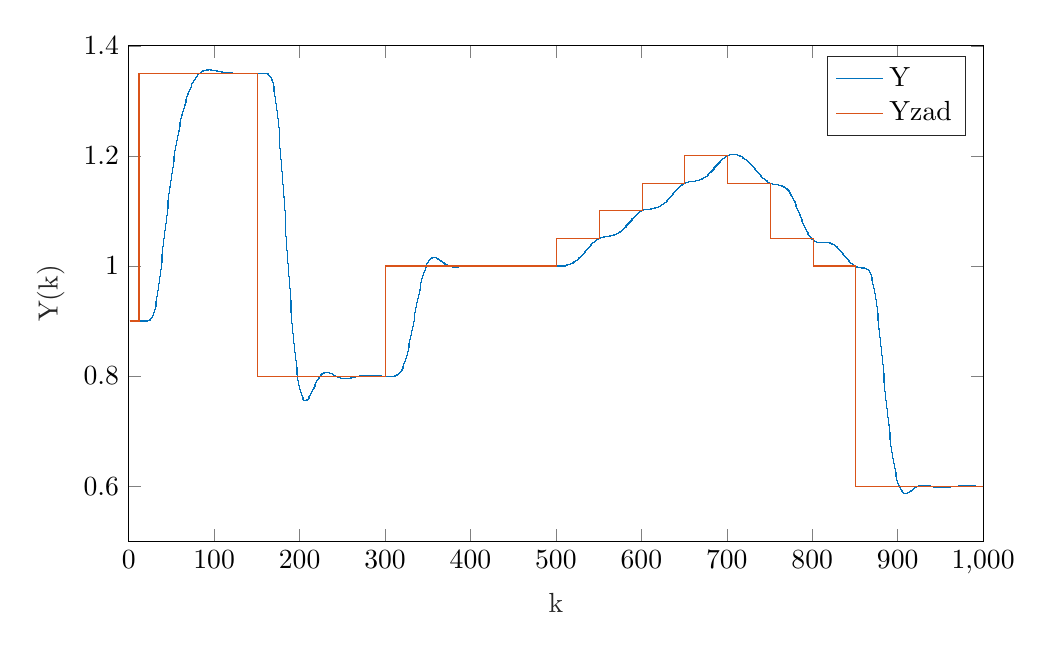
\begin{tikzpicture}

\begin{axis}[%
width=4.272in,
height=2.477in,
at={(0.717in,0.437in)},
scale only axis,
xmin=0,
xmax=1000,
xlabel style={font=\color{white!15!black}},
xlabel={k},
ymin=0.5,
ymax=1.4,
ylabel style={font=\color{white!15!black}},
ylabel={Y(k)},
axis background/.style={fill=white},
legend style={legend cell align=left, align=left, draw=white!15!black}
]
\addplot[const plot, color=mycolor1] table[row sep=crcr] {%
1	0.9\\
2	0.9\\
3	0.9\\
4	0.9\\
5	0.9\\
6	0.9\\
7	0.9\\
8	0.9\\
9	0.9\\
10	0.9\\
11	0.9\\
12	0.9\\
13	0.9\\
14	0.9\\
15	0.9\\
16	0.9\\
17	0.9\\
18	0.9\\
19	0.9\\
20	0.9\\
21	0.9\\
22	0.9003968325\\
23	0.90110505465075\\
24	0.901851548804444\\
25	0.902926732649044\\
26	0.9045740507257\\
27	0.906995673734868\\
28	0.910357581452216\\
29	0.91479409195594\\
30	0.92041189372332\\
31	0.927293631597811\\
32	0.935481917271842\\
33	0.944987479442384\\
34	0.955752143856375\\
35	0.967585143897724\\
36	0.980245690511738\\
37	0.993524900254613\\
38	1.00724220273058\\
39	1.02124212187654\\
40	1.03539139393444\\
41	1.04957638853821\\
42	1.06370080258905\\
43	1.07768359953247\\
44	1.09145716931113\\
45	1.10496568667539\\
46	1.11816364771215\\
47	1.13101456642337\\
48	1.1434898149686\\
49	1.15556759279779\\
50	1.16723201135847\\
51	1.17847228237882\\
52	1.18928199891931\\
53	1.19965849946121\\
54	1.20960230627283\\
55	1.21911663017192\\
56	1.22820693459549\\
57	1.23688055260421\\
58	1.24514635109392\\
59	1.25301443706996\\
60	1.26049590136546\\
61	1.26760259565856\\
62	1.27434693907117\\
63	1.28074174608457\\
64	1.28679954411603\\
65	1.29253204733993\\
66	1.29795023797434\\
67	1.3030644413896\\
68	1.3078843950437\\
69	1.31241931135295\\
70	1.31667793468543\\
71	1.32066859272397\\
72	1.32439924248811\\
73	1.32787751157148\\
74	1.33111076093811\\
75	1.33410618724198\\
76	1.33687093004876\\
77	1.33941215850932\\
78	1.34173714007823\\
79	1.34385329361559\\
80	1.34576822897515\\
81	1.34748977496456\\
82	1.34902599736423\\
83	1.3503852084965\\
84	1.35157596840274\\
85	1.35260707550363\\
86	1.35348754538761\\
87	1.35422657910142\\
88	1.3548335232566\\
89	1.35531782394082\\
90	1.35568897613632\\
91	1.35595647009444\\
92	1.35612973589315\\
93	1.35621808720922\\
94	1.35623066522872\\
95	1.35617638368734\\
96	1.35606387616748\\
97	1.35590144675004\\
98	1.35569702492415\\
99	1.35545812544111\\
100	1.35519181361515\\
101	1.35490467641866\\
102	1.35460279958943\\
103	1.35429175085935\\
104	1.35397656932081\\
105	1.35366176085724\\
106	1.35335129946519\\
107	1.35304863419235\\
108	1.35275670132403\\
109	1.35247794137879\\
110	1.35221432042028\\
111	1.35196735515504\\
112	1.35173814126113\\
113	1.35152738437876\\
114	1.35133543318901\\
115	1.35116231400986\\
116	1.35100776635043\\
117	1.35087127888471\\
118	1.35075212533525\\
119	1.35064939979385\\
120	1.35056205104808\\
121	1.35048891552808\\
122	1.35042874853686\\
123	1.35038025347687\\
124	1.35034210883664\\
125	1.35031299275196\\
126	1.35029160500585\\
127	1.3502766863805\\
128	1.35026703532044\\
129	1.35026152190965\\
130	1.35025909920554\\
131	1.35025881200833\\
132	1.35025980317699\\
133	1.35026131763001\\
134	1.3502627041929\\
135	1.35026341547329\\
136	1.35026300595865\\
137	1.35026112854246\\
138	1.35025752969034\\
139	1.35025204346031\\
140	1.35024458458987\\
141	1.35023514085807\\
142	1.35022376492329\\
143	1.35021056582744\\
144	1.35019570034494\\
145	1.35017936434093\\
146	1.35016178428769\\
147	1.35014320907172\\
148	1.35012390220676\\
149	1.35010413455032\\
150	1.35008417760403\\
151	1.35006429746031\\
152	1.35004474944139\\
153	1.35002577346057\\
154	1.35000759012025\\
155	1.34999039754741\\
156	1.34997436895457\\
157	1.34995965090253\\
158	1.34994636223132\\
159	1.34993459361745\\
160	1.34992440770813\\
161	1.34951889923522\\
162	1.34880333328902\\
163	1.34801637133565\\
164	1.34680623564434\\
165	1.34487818982496\\
166	1.34198761101855\\
167	1.33793381210464\\
168	1.33255453756716\\
169	1.32572106414159\\
170	1.31733384413307\\
171	1.30733781596696\\
172	1.29571365605078\\
173	1.2824452175893\\
174	1.26753853904809\\
175	1.25104365760431\\
176	1.23304727100621\\
177	1.21366635998876\\
178	1.19304265516873\\
179	1.1713378458413\\
180	1.14872944006864\\
181	1.12540626923593\\
182	1.10156388099674\\
183	1.07740205013679\\
184	1.05312296740804\\
185	1.02892759572966\\
186	1.00501147782133\\
187	0.98156127181985\\
188	0.958751911430767\\
189	0.936744301032577\\
190	0.915683468219405\\
191	0.895697151551403\\
192	0.87689483720541\\
193	0.859367140555324\\
194	0.843185398442461\\
195	0.828401526929037\\
196	0.815048252072926\\
197	0.803139700616667\\
198	0.792672284955702\\
199	0.783625826910249\\
200	0.775964873487657\\
201	0.769640163035288\\
202	0.764590200971363\\
203	0.760742909007944\\
204	0.758017323223758\\
205	0.75632531988144\\
206	0.755573340172202\\
207	0.755664080816826\\
208	0.75649812124768\\
209	0.757975463734339\\
210	0.759996967501476\\
211	0.762465661879657\\
212	0.765287927215516\\
213	0.768374535670495\\
214	0.771641546661306\\
215	0.775011053627311\\
216	0.778411780963361\\
217	0.781779532677985\\
218	0.785057497075944\\
219	0.78819641406661\\
220	0.791154613532383\\
221	0.793897934635967\\
222	0.79639953705089\\
223	0.798639615895301\\
224	0.800605032685999\\
225	0.802288874976543\\
226	0.803689957519954\\
227	0.804812277764049\\
228	0.805664438217677\\
229	0.80625904773855\\
230	0.806612113128949\\
231	0.80674243162307\\
232	0.806670993941009\\
233	0.806420406597751\\
234	0.806014341115425\\
235	0.805477016712229\\
236	0.804832721946634\\
237	0.80410537969662\\
238	0.803318158769883\\
239	0.802493134391884\\
240	0.801650998821049\\
241	0.800810822407754\\
242	0.799989864555977\\
243	0.799203433271251\\
244	0.798464791291063\\
245	0.79778510619742\\
246	0.797173441408183\\
247	0.796636784534522\\
248	0.796180109276034\\
249	0.795806466800069\\
250	0.795517102413963\\
251	0.795311593282831\\
252	0.795188002965221\\
253	0.795143048627405\\
254	0.795172276946966\\
255	0.795270244919908\\
256	0.795430702034841\\
257	0.795646770564863\\
258	0.795911121044516\\
259	0.796216140337837\\
260	0.796554090056421\\
261	0.796917253446428\\
262	0.797298069223946\\
263	0.797689251192951\\
264	0.798083892823816\\
265	0.79847555629814\\
266	0.798858345833424\\
267	0.799226965385318\\
268	0.799576761083186\\
269	0.799903748984284\\
270	0.800204628931693\\
271	0.800476785470349\\
272	0.800718276913917\\
273	0.800927813763172\\
274	0.801104727754768\\
275	0.801248932869047\\
276	0.801360879648473\\
277	0.801441504176269\\
278	0.801492173040124\\
279	0.801514625560706\\
280	0.801510914501775\\
281	0.801483346400498\\
282	0.801434422565709\\
283	0.801366781691079\\
284	0.801283144921891\\
285	0.80118626410091\\
286	0.80107887380304\\
287	0.80096364765217\\
288	0.800843159298981\\
289	0.800719848327149\\
290	0.800595991249099\\
291	0.800473677652468\\
292	0.800354791466003\\
293	0.800240997229543\\
294	0.800133731177851\\
295	0.800034196882735\\
296	0.799943365142501\\
297	0.799861977762359\\
298	0.799790554833885\\
299	0.799729405095798\\
300	0.799678638941685\\
301	0.799638183632529\\
302	0.799607800272158\\
303	0.799587102111522\\
304	0.799575573762118\\
305	0.79957259091919\\
306	0.799577440220629\\
307	0.799589338896979\\
308	0.799607453900748\\
309	0.799630920238458\\
310	0.799658858265823\\
311	0.800087252030063\\
312	0.800829896899739\\
313	0.801526913554124\\
314	0.802314448958003\\
315	0.803306971242467\\
316	0.804599897685075\\
317	0.80627193853803\\
318	0.808387185421943\\
319	0.810996970220403\\
320	0.814141517893137\\
321	0.817832237576928\\
322	0.822058342893119\\
323	0.82682333598127\\
324	0.832134339197458\\
325	0.837981296502411\\
326	0.844339788339714\\
327	0.851173479010461\\
328	0.858436240883071\\
329	0.866073994644319\\
330	0.874026300243561\\
331	0.882228655782662\\
332	0.890615216678407\\
333	0.899119386465001\\
334	0.907673219149908\\
335	0.916208290634322\\
336	0.924657350987353\\
337	0.932955694514448\\
338	0.941042287608186\\
339	0.948860689023248\\
340	0.956359792560657\\
341	0.963494373316752\\
342	0.970225388345921\\
343	0.976520118682778\\
344	0.982352309401972\\
345	0.98770229142151\\
346	0.992556980678792\\
347	0.996909733881368\\
348	1.00076008658177\\
349	1.00411339535527\\
350	1.00698040247153\\
351	1.00937674072753\\
352	1.01132239913817\\
353	1.01284116803809\\
354	1.0139600704795\\
355	1.01470878044002\\
356	1.01511903420175\\
357	1.01522404704477\\
358	1.01505794707236\\
359	1.0146552357442\\
360	1.01405028282807\\
361	1.01327686182708\\
362	1.01236773018765\\
363	1.01135425681932\\
364	1.01026609835369\\
365	1.00913092530819\\
366	1.0079741990589\\
367	1.00681899971261\\
368	1.0056859039023\\
369	1.00459291058741\\
370	1.00355541218626\\
371	1.00258620777425\\
372	1.00169555464129\\
373	1.00089125422008\\
374	1.00017876824074\\
375	0.999561360866317\\
376	0.99904026247886\\
377	0.99861485074555\\
378	0.998282844636035\\
379	0.998040507192143\\
380	0.997882853054599\\
381	0.997803857012575\\
382	0.99779666014669\\
383	0.997853770470491\\
384	0.997967255326939\\
385	0.998128923157442\\
386	0.998330492628963\\
387	0.99856374747751\\
388	0.998820675798544\\
389	0.99909359287906\\
390	0.99937524701533\\
391	0.999658908088884\\
392	0.999938438976968\\
393	1.00020835014948\\
394	1.00046383805041\\
395	1.00070080807695\\
396	1.0009158831536\\
397	1.00110639905052\\
398	1.00127038771589\\
399	1.00140654998108\\
400	1.00151421905542\\
401	1.00159331625788\\
402	1.00164430043515\\
403	1.00166811249474\\
404	1.00166611643787\\
405	1.00164003821447\\
406	1.00159190364311\\
407	1.00152397654534\\
408	1.00143869813951\\
409	1.00133862862597\\
410	1.00122639177664\\
411	1.00110462321982\\
412	1.00097592298746\\
413	1.00084281277039\\
414	1.00070769820757\\
415	1.00057283642144\\
416	1.00044030890337\\
417	1.00031199975319\\
418	1.00018957918462\\
419	1.00007449212675\\
420	0.999967951678888\\
421	0.999870937114806\\
422	0.999784196080508\\
423	0.999708250589163\\
424	0.99964340638599\\
425	0.999589765235247\\
426	0.999547239670111\\
427	0.99951556974366\\
428	0.999494341324697\\
429	0.99948300549489\\
430	0.999480898622941\\
431	0.999487262716258\\
432	0.999501265680006\\
433	0.99952202114661\\
434	0.999548607574855\\
435	0.999580086355753\\
436	0.999615518701678\\
437	0.999653981134935\\
438	0.999694579431357\\
439	0.999736460913058\\
440	0.999778825021436\\
441	0.999820932136559\\
442	0.999862110641679\\
443	0.999901762261401\\
444	0.999939365728923\\
445	0.999974478861247\\
446	1.0000067391416\\
447	1.00003586292502\\
448	1.00006164339664\\
449	1.00008394742205\\
450	1.0001027114364\\
451	1.0001179365222\\
452	1.0001296828272\\
453	1.00013806347171\\
454	1.00014323809091\\
455	1.00014540615114\\
456	1.00014480017174\\
457	1.0001416789738\\
458	1.00013632106689\\
459	1.0001290182729\\
460	1.00012006967369\\
461	1.00010977595652\\
462	1.00009843421817\\
463	1.00008633327581\\
464	1.00007374952002\\
465	1.00006094333331\\
466	1.0000481560859\\
467	1.00003560770982\\
468	1.00002349484263\\
469	1.00001198952323\\
470	1.00000123841427\\
471	0.999991362519225\\
472	0.999982457356436\\
473	0.999974593547984\\
474	0.999967817777953\\
475	0.999962154072194\\
476	0.999957605350476\\
477	0.999954155201463\\
478	0.999951769831483\\
479	0.999950400139309\\
480	0.999949983871121\\
481	0.99995044781243\\
482	0.999951709976786\\
483	0.999953681754603\\
484	0.999956269989249\\
485	0.999959378951586\\
486	0.999962912188326\\
487	0.999966774223801\\
488	0.999970872098985\\
489	0.999975116735722\\
490	0.999979424118093\\
491	0.99998371628665\\
492	0.999987922144747\\
493	0.999991978079466\\
494	0.99999582840252\\
495	0.99999942561911\\
496	1.00000273053496\\
497	1.00000571221353\\
498	1.00000834779705\\
499	1.00001062220599\\
500	1.00001252773249\\
501	1.00001406354371\\
502	1.00001523511121\\
503	1.00001605358234\\
504	1.00001653510923\\
505	1.00001670015035\\
506	1.0000165727588\\
507	1.00001617987058\\
508	1.00001555060467\\
509	1.00001471558604\\
510	1.00001370630078\\
511	1.00040938687002\\
512	1.00111634385559\\
513	1.00172392016373\\
514	1.00227704645393\\
515	1.00281406265013\\
516	1.00336749042988\\
517	1.00396472359866\\
518	1.00462864462469\\
519	1.005378174803\\
520	1.00622876478752\\
521	1.0071736562442\\
522	1.00818959391501\\
523	1.00927499574596\\
524	1.01044285867689\\
525	1.01170039690845\\
526	1.01304992484452\\
527	1.01448962762909\\
528	1.01601423267138\\
529	1.01761559400932\\
530	1.01928319999231\\
531	1.0210055401198\\
532	1.02277202429034\\
533	1.0245727687922\\
534	1.02639697486112\\
535	1.02823262041945\\
536	1.0300670318369\\
537	1.03188736390347\\
538	1.03368100073895\\
539	1.03543588868484\\
540	1.03714081076041\\
541	1.03878556621624\\
542	1.04036099084052\\
543	1.04185889769697\\
544	1.0432721046191\\
545	1.0445945486784\\
546	1.04582138463271\\
547	1.04694903207134\\
548	1.04797517997097\\
549	1.04889875606294\\
550	1.04971986728836\\
551	1.05043971882005\\
552	1.05106052379489\\
553	1.05158541486351\\
554	1.05201835689525\\
555	1.05236405258994\\
556	1.05262783779425\\
557	1.05281556975452\\
558	1.05293351269471\\
559	1.05298822431716\\
560	1.05298644616155\\
561	1.05333263244468\\
562	1.05394921456856\\
563	1.05443231932367\\
564	1.05483302951003\\
565	1.05519562267473\\
566	1.05555827515993\\
567	1.05595369385869\\
568	1.05640968435715\\
569	1.05694966297499\\
570	1.05759311919599\\
571	1.05833682011125\\
572	1.05916046354588\\
573	1.06006488133588\\
574	1.06106501687024\\
575	1.06216959444918\\
576	1.06338201723138\\
577	1.06470115866325\\
578	1.06612205987656\\
579	1.06763654398343\\
580	1.06923375684288\\
581	1.07090157113358\\
582	1.07262854843728\\
583	1.07440376931444\\
584	1.07621525118013\\
585	1.07804967488953\\
586	1.07989298958076\\
587	1.08173092445078\\
588	1.08354941970057\\
589	1.08533498728995\\
590	1.0870750107602\\
591	1.0887579473229\\
592	1.09037336741601\\
593	1.09191191109257\\
594	1.09336532773929\\
595	1.09472659976837\\
596	1.09599004756228\\
597	1.09715138050907\\
598	1.09820770296188\\
599	1.09915748268227\\
600	1.1000004882354\\
601	1.10073770303673\\
602	1.10137122845058\\
603	1.10190418733924\\
604	1.10234062769767\\
605	1.10268541839338\\
606	1.10294413404599\\
607	1.10312293249677\\
608	1.1032284294665\\
609	1.10326757419677\\
610	1.10324752919333\\
611	1.10357322078997\\
612	1.10416755575576\\
613	1.10462710229684\\
614	1.10500337757068\\
615	1.1053410795647\\
616	1.10567878457563\\
617	1.10604957333897\\
618	1.10648159450064\\
619	1.10699857293944\\
620	1.10762026941351\\
621	1.10834368157685\\
622	1.10914869493528\\
623	1.11003628786775\\
624	1.11102151121821\\
625	1.11211315872286\\
626	1.11331466659475\\
627	1.1146249071052\\
628	1.11603888856487\\
629	1.1175483725503\\
630	1.11914241786794\\
631	1.12080878808583\\
632	1.12253591731215\\
633	1.12431274396181\\
634	1.12612713213262\\
635	1.12796560154174\\
636	1.12981393559359\\
637	1.1316576962092\\
638	1.13348265761338\\
639	1.13527516968724\\
640	1.13702246011925\\
641	1.1387128385308\\
642	1.14033573775641\\
643	1.14188167163494\\
644	1.1433422758195\\
645	1.1447104322657\\
646	1.145980374691\\
647	1.14714773985568\\
648	1.14820957351633\\
649	1.14916429863164\\
650	1.15001165231066\\
651	1.15075259922795\\
652	1.15138923393206\\
653	1.15192468347357\\
654	1.15236301001512\\
655	1.15270910546886\\
656	1.15296857522063\\
657	1.15314761441455\\
658	1.15325288141846\\
659	1.15329137228585\\
660	1.15327029935151\\
661	1.15359464542537\\
662	1.15418737495578\\
663	1.15464510835916\\
664	1.15501941276866\\
665	1.15535503460211\\
666	1.155690596331\\
667	1.15605922200227\\
668	1.15648910020565\\
669	1.1570039919949\\
670	1.1576236902334\\
671	1.15834522017804\\
672	1.1591484900928\\
673	1.16003449649167\\
674	1.16101830408993\\
675	1.16210871639956\\
676	1.16330917547781\\
677	1.16461855572892\\
678	1.1660318641527\\
679	1.16754085787656\\
680	1.16913458845456\\
681	1.17080080976581\\
682	1.17252794419407\\
683	1.17430491679859\\
684	1.17611957706646\\
685	1.17795842920068\\
686	1.17980724052501\\
687	1.18165155663356\\
688	1.183477135477\\
689	1.18527031098941\\
690	1.18701829548606\\
691	1.1887093840055\\
692	1.19033299577327\\
693	1.19187963214186\\
694	1.19334091751603\\
695	1.1947097239258\\
696	1.19598027654118\\
697	1.1971482049811\\
698	1.19821054926872\\
699	1.19916572801499\\
700	1.20001347532299\\
701	1.20075475413974\\
702	1.20139165848492\\
703	1.20192731598551\\
704	1.20236579038155\\
705	1.20271197605165\\
706	1.20297148161954\\
707	1.20315050611813\\
708	1.2032557123336\\
709	1.20329410114738\\
710	1.20327289001505\\
711	1.20280340246781\\
712	1.20197949443207\\
713	1.20121916410976\\
714	1.20048418239853\\
715	1.19974267734762\\
716	1.19896828523762\\
717	1.19813939477381\\
718	1.19723847653431\\
719	1.19625149024025\\
720	1.19516736283582\\
721	1.1939966656711\\
722	1.19276584118506\\
723	1.19147906815355\\
724	1.19012543003654\\
725	1.18869930913946\\
726	1.18719952083662\\
727	1.18562856671054\\
728	1.18399199220324\\
729	1.18229783590438\\
730	1.18055615898757\\
731	1.17877771994491\\
732	1.17697210277387\\
733	1.17514797964956\\
734	1.17331477603314\\
735	1.17148301795\\
736	1.16966379732088\\
737	1.16786832757869\\
738	1.16610757631066\\
739	1.16439196343536\\
740	1.16273111497917\\
741	1.16113370855843\\
742	1.15960747443339\\
743	1.15815927213312\\
744	1.1567950765124\\
745	1.15551987346826\\
746	1.15433756859892\\
747	1.15325094422691\\
748	1.15226165621367\\
749	1.15137026334976\\
750	1.15057628326406\\
751	1.14987826762436\\
752	1.14927388477541\\
753	1.14875999903333\\
754	1.14833274762912\\
755	1.14798762385052\\
756	1.14771956985092\\
757	1.14752307614174\\
758	1.14739228361596\\
759	1.14732108472827\\
760	1.14730322110229\\
761	1.14693478039478\\
762	1.14629387728537\\
763	1.14576769479887\\
764	1.1452749569674\\
765	1.14474622511151\\
766	1.14412257054753\\
767	1.1433543874333\\
768	1.14240033028543\\
769	1.14122636251588\\
770	1.13980490394141\\
771	1.13813327881775\\
772	1.13622775539906\\
773	1.13408590561064\\
774	1.13169482228744\\
775	1.12905159646821\\
776	1.12616177549122\\
777	1.12303801303747\\
778	1.11969888827224\\
779	1.1161678739883\\
780	1.1124724360704\\
781	1.10864232036899\\
782	1.10470732601222\\
783	1.10069720924071\\
784	1.09664292622671\\
785	1.0925765150098\\
786	1.08853013218155\\
787	1.08453524608933\\
788	1.08062196520243\\
789	1.07681848310651\\
790	1.07315062404299\\
791	1.06964151989627\\
792	1.06631147833079\\
793	1.0631779602663\\
794	1.06025550341444\\
795	1.05755559675842\\
796	1.05508660916733\\
797	1.05285380248214\\
798	1.05085941456476\\
799	1.04910279996318\\
800	1.04758061769505\\
801	1.04628705506404\\
802	1.0452140722705\\
803	1.044351653951\\
804	1.04368806551219\\
805	1.0432101193333\\
806	1.04290345062832\\
807	1.04275279655942\\
808	1.04274227153947\\
809	1.04285563294737\\
810	1.04307653255715\\
811	1.04299140055327\\
812	1.04266965616485\\
813	1.04250699534601\\
814	1.04244392825164\\
815	1.04242839530598\\
816	1.04241511838254\\
817	1.04236500994948\\
818	1.04224463192628\\
819	1.0420256973767\\
820	1.04168460935379\\
821	1.04122123254866\\
822	1.04065317567022\\
823	1.03997755132816\\
824	1.0391780176565\\
825	1.03824509623151\\
826	1.03717522005222\\
827	1.03596988412573\\
828	1.03463488734745\\
829	1.03317965587997\\
830	1.03161663952905\\
831	1.02995984594171\\
832	1.02822282091232\\
833	1.02641876520716\\
834	1.02456206402348\\
835	1.02266850710263\\
836	1.02075463337065\\
837	1.01883717345544\\
838	1.01693257809918\\
839	1.01505662198516\\
840	1.01322407378949\\
841	1.01144846921064\\
842	1.00974205151795\\
843	1.00811579985152\\
844	1.00657937856382\\
845	1.00514100699203\\
846	1.00380735230144\\
847	1.00258348023216\\
848	1.00147285448576\\
849	1.00047737674732\\
850	0.999597460423544\\
851	0.998832129947184\\
852	0.998179132813485\\
853	0.997635052547799\\
854	0.99719542259527\\
855	0.996854848745601\\
856	0.996607142692001\\
857	0.996445462924645\\
858	0.996362458044904\\
859	0.996350408427594\\
860	0.996401362874079\\
861	0.996109629816194\\
862	0.995551614064934\\
863	0.995009666148765\\
864	0.994216691386937\\
865	0.992947798135629\\
866	0.991015297256109\\
867	0.988264238824071\\
868	0.984568429788473\\
869	0.979826882167447\\
870	0.973960646650634\\
871	0.966929205462071\\
872	0.958722682741073\\
873	0.949327563251365\\
874	0.938742061889922\\
875	0.926997470478845\\
876	0.914152732667802\\
877	0.900289718232804\\
878	0.885526609339621\\
879	0.870048740470661\\
880	0.854065600402944\\
881	0.837757545633109\\
882	0.821279147033163\\
883	0.804762184475895\\
884	0.788321943064686\\
885	0.772069348052869\\
886	0.756116297553503\\
887	0.740572555930676\\
888	0.725542316593946\\
889	0.711118753508792\\
890	0.697379335889381\\
891	0.684385756488678\\
892	0.672186159185987\\
893	0.660817075710471\\
894	0.650304933391636\\
895	0.640666706305716\\
896	0.631909779237839\\
897	0.62403174813625\\
898	0.617020556497771\\
899	0.610855074757561\\
900	0.605506172482791\\
901	0.600938020907226\\
902	0.597109302249915\\
903	0.593974236039276\\
904	0.591483458059632\\
905	0.589584813766831\\
906	0.588224143381368\\
907	0.587346096947157\\
908	0.586894964978029\\
909	0.586815487083717\\
910	0.587053594013179\\
911	0.587557049286112\\
912	0.588275984373666\\
913	0.5891633404078\\
914	0.590175231538074\\
915	0.591271240227415\\
916	0.592414648094076\\
917	0.593572600485164\\
918	0.594716201925493\\
919	0.595820542082976\\
920	0.596864655766684\\
921	0.597831424121497\\
922	0.598707425980132\\
923	0.599482747943879\\
924	0.600150760422345\\
925	0.600707865682163\\
926	0.60115322333697\\
927	0.601488458671674\\
928	0.60171735945684\\
929	0.601845567099499\\
930	0.601880267866927\\
931	0.601829889460008\\
932	0.601703807504322\\
933	0.601512065760973\\
934	0.601265113179839\\
935	0.60097356035893\\
936	0.600647957498086\\
937	0.600298595488258\\
938	0.599935331317265\\
939	0.599567438488636\\
940	0.599203482659606\\
941	0.598851222237878\\
942	0.598517533261986\\
943	0.598208357540609\\
944	0.597928672739817\\
945	0.597682482873989\\
946	0.597472827466267\\
947	0.597301807492771\\
948	0.597170626110886\\
949	0.597079642097725\\
950	0.597028433891878\\
951	0.597015872139279\\
952	0.597040198688923\\
953	0.597099110061235\\
954	0.597189843515262\\
955	0.597309263965637\\
956	0.597453950142212\\
957	0.597620278541056\\
958	0.597804503881963\\
959	0.598002834961496\\
960	0.598211504968482\\
961	0.598426835507268\\
962	0.598645293749683\\
963	0.598863542306555\\
964	0.599078481571407\\
965	0.599287284440605\\
966	0.599487423454155\\
967	0.599676690528423\\
968	0.599853209565049\\
969	0.600015442318847\\
970	0.60016218799078\\
971	0.600292577080268\\
972	0.600406060084125\\
973	0.600502391667822\\
974	0.600581610959129\\
975	0.600644018625313\\
976	0.600690151394004\\
977	0.600720754665501\\
978	0.600736753842057\\
979	0.600739224968596\\
980	0.60072936524077\\
981	0.600708463891536\\
982	0.600677873917782\\
983	0.60063898505529\\
984	0.600593198354631\\
985	0.600541902653678\\
986	0.600486453185301\\
987	0.600428152502531\\
988	0.600368233848821\\
989	0.600307847048944\\
990	0.600248046947038\\
991	0.600189784373033\\
992	0.600133899577584\\
993	0.600081118039004\\
994	0.600032048513815\\
995	0.599987183175549\\
996	0.599946899664326\\
997	0.599911464852545\\
998	0.599881040119561\\
999	0.599855687920309\\
1000	0.599835379429238\\
};
\addlegendentry{Y}

\addplot[const plot, color=mycolor2] table[row sep=crcr] {%
1	0.9\\
2	0.9\\
3	0.9\\
4	0.9\\
5	0.9\\
6	0.9\\
7	0.9\\
8	0.9\\
9	0.9\\
10	0.9\\
11	0.9\\
12	1.35\\
13	1.35\\
14	1.35\\
15	1.35\\
16	1.35\\
17	1.35\\
18	1.35\\
19	1.35\\
20	1.35\\
21	1.35\\
22	1.35\\
23	1.35\\
24	1.35\\
25	1.35\\
26	1.35\\
27	1.35\\
28	1.35\\
29	1.35\\
30	1.35\\
31	1.35\\
32	1.35\\
33	1.35\\
34	1.35\\
35	1.35\\
36	1.35\\
37	1.35\\
38	1.35\\
39	1.35\\
40	1.35\\
41	1.35\\
42	1.35\\
43	1.35\\
44	1.35\\
45	1.35\\
46	1.35\\
47	1.35\\
48	1.35\\
49	1.35\\
50	1.35\\
51	1.35\\
52	1.35\\
53	1.35\\
54	1.35\\
55	1.35\\
56	1.35\\
57	1.35\\
58	1.35\\
59	1.35\\
60	1.35\\
61	1.35\\
62	1.35\\
63	1.35\\
64	1.35\\
65	1.35\\
66	1.35\\
67	1.35\\
68	1.35\\
69	1.35\\
70	1.35\\
71	1.35\\
72	1.35\\
73	1.35\\
74	1.35\\
75	1.35\\
76	1.35\\
77	1.35\\
78	1.35\\
79	1.35\\
80	1.35\\
81	1.35\\
82	1.35\\
83	1.35\\
84	1.35\\
85	1.35\\
86	1.35\\
87	1.35\\
88	1.35\\
89	1.35\\
90	1.35\\
91	1.35\\
92	1.35\\
93	1.35\\
94	1.35\\
95	1.35\\
96	1.35\\
97	1.35\\
98	1.35\\
99	1.35\\
100	1.35\\
101	1.35\\
102	1.35\\
103	1.35\\
104	1.35\\
105	1.35\\
106	1.35\\
107	1.35\\
108	1.35\\
109	1.35\\
110	1.35\\
111	1.35\\
112	1.35\\
113	1.35\\
114	1.35\\
115	1.35\\
116	1.35\\
117	1.35\\
118	1.35\\
119	1.35\\
120	1.35\\
121	1.35\\
122	1.35\\
123	1.35\\
124	1.35\\
125	1.35\\
126	1.35\\
127	1.35\\
128	1.35\\
129	1.35\\
130	1.35\\
131	1.35\\
132	1.35\\
133	1.35\\
134	1.35\\
135	1.35\\
136	1.35\\
137	1.35\\
138	1.35\\
139	1.35\\
140	1.35\\
141	1.35\\
142	1.35\\
143	1.35\\
144	1.35\\
145	1.35\\
146	1.35\\
147	1.35\\
148	1.35\\
149	1.35\\
150	1.35\\
151	0.8\\
152	0.8\\
153	0.8\\
154	0.8\\
155	0.8\\
156	0.8\\
157	0.8\\
158	0.8\\
159	0.8\\
160	0.8\\
161	0.8\\
162	0.8\\
163	0.8\\
164	0.8\\
165	0.8\\
166	0.8\\
167	0.8\\
168	0.8\\
169	0.8\\
170	0.8\\
171	0.8\\
172	0.8\\
173	0.8\\
174	0.8\\
175	0.8\\
176	0.8\\
177	0.8\\
178	0.8\\
179	0.8\\
180	0.8\\
181	0.8\\
182	0.8\\
183	0.8\\
184	0.8\\
185	0.8\\
186	0.8\\
187	0.8\\
188	0.8\\
189	0.8\\
190	0.8\\
191	0.8\\
192	0.8\\
193	0.8\\
194	0.8\\
195	0.8\\
196	0.8\\
197	0.8\\
198	0.8\\
199	0.8\\
200	0.8\\
201	0.8\\
202	0.8\\
203	0.8\\
204	0.8\\
205	0.8\\
206	0.8\\
207	0.8\\
208	0.8\\
209	0.8\\
210	0.8\\
211	0.8\\
212	0.8\\
213	0.8\\
214	0.8\\
215	0.8\\
216	0.8\\
217	0.8\\
218	0.8\\
219	0.8\\
220	0.8\\
221	0.8\\
222	0.8\\
223	0.8\\
224	0.8\\
225	0.8\\
226	0.8\\
227	0.8\\
228	0.8\\
229	0.8\\
230	0.8\\
231	0.8\\
232	0.8\\
233	0.8\\
234	0.8\\
235	0.8\\
236	0.8\\
237	0.8\\
238	0.8\\
239	0.8\\
240	0.8\\
241	0.8\\
242	0.8\\
243	0.8\\
244	0.8\\
245	0.8\\
246	0.8\\
247	0.8\\
248	0.8\\
249	0.8\\
250	0.8\\
251	0.8\\
252	0.8\\
253	0.8\\
254	0.8\\
255	0.8\\
256	0.8\\
257	0.8\\
258	0.8\\
259	0.8\\
260	0.8\\
261	0.8\\
262	0.8\\
263	0.8\\
264	0.8\\
265	0.8\\
266	0.8\\
267	0.8\\
268	0.8\\
269	0.8\\
270	0.8\\
271	0.8\\
272	0.8\\
273	0.8\\
274	0.8\\
275	0.8\\
276	0.8\\
277	0.8\\
278	0.8\\
279	0.8\\
280	0.8\\
281	0.8\\
282	0.8\\
283	0.8\\
284	0.8\\
285	0.8\\
286	0.8\\
287	0.8\\
288	0.8\\
289	0.8\\
290	0.8\\
291	0.8\\
292	0.8\\
293	0.8\\
294	0.8\\
295	0.8\\
296	0.8\\
297	0.8\\
298	0.8\\
299	0.8\\
300	0.8\\
301	1\\
302	1\\
303	1\\
304	1\\
305	1\\
306	1\\
307	1\\
308	1\\
309	1\\
310	1\\
311	1\\
312	1\\
313	1\\
314	1\\
315	1\\
316	1\\
317	1\\
318	1\\
319	1\\
320	1\\
321	1\\
322	1\\
323	1\\
324	1\\
325	1\\
326	1\\
327	1\\
328	1\\
329	1\\
330	1\\
331	1\\
332	1\\
333	1\\
334	1\\
335	1\\
336	1\\
337	1\\
338	1\\
339	1\\
340	1\\
341	1\\
342	1\\
343	1\\
344	1\\
345	1\\
346	1\\
347	1\\
348	1\\
349	1\\
350	1\\
351	1\\
352	1\\
353	1\\
354	1\\
355	1\\
356	1\\
357	1\\
358	1\\
359	1\\
360	1\\
361	1\\
362	1\\
363	1\\
364	1\\
365	1\\
366	1\\
367	1\\
368	1\\
369	1\\
370	1\\
371	1\\
372	1\\
373	1\\
374	1\\
375	1\\
376	1\\
377	1\\
378	1\\
379	1\\
380	1\\
381	1\\
382	1\\
383	1\\
384	1\\
385	1\\
386	1\\
387	1\\
388	1\\
389	1\\
390	1\\
391	1\\
392	1\\
393	1\\
394	1\\
395	1\\
396	1\\
397	1\\
398	1\\
399	1\\
400	1\\
401	1\\
402	1\\
403	1\\
404	1\\
405	1\\
406	1\\
407	1\\
408	1\\
409	1\\
410	1\\
411	1\\
412	1\\
413	1\\
414	1\\
415	1\\
416	1\\
417	1\\
418	1\\
419	1\\
420	1\\
421	1\\
422	1\\
423	1\\
424	1\\
425	1\\
426	1\\
427	1\\
428	1\\
429	1\\
430	1\\
431	1\\
432	1\\
433	1\\
434	1\\
435	1\\
436	1\\
437	1\\
438	1\\
439	1\\
440	1\\
441	1\\
442	1\\
443	1\\
444	1\\
445	1\\
446	1\\
447	1\\
448	1\\
449	1\\
450	1\\
451	1\\
452	1\\
453	1\\
454	1\\
455	1\\
456	1\\
457	1\\
458	1\\
459	1\\
460	1\\
461	1\\
462	1\\
463	1\\
464	1\\
465	1\\
466	1\\
467	1\\
468	1\\
469	1\\
470	1\\
471	1\\
472	1\\
473	1\\
474	1\\
475	1\\
476	1\\
477	1\\
478	1\\
479	1\\
480	1\\
481	1\\
482	1\\
483	1\\
484	1\\
485	1\\
486	1\\
487	1\\
488	1\\
489	1\\
490	1\\
491	1\\
492	1\\
493	1\\
494	1\\
495	1\\
496	1\\
497	1\\
498	1\\
499	1\\
500	1\\
501	1.05\\
502	1.05\\
503	1.05\\
504	1.05\\
505	1.05\\
506	1.05\\
507	1.05\\
508	1.05\\
509	1.05\\
510	1.05\\
511	1.05\\
512	1.05\\
513	1.05\\
514	1.05\\
515	1.05\\
516	1.05\\
517	1.05\\
518	1.05\\
519	1.05\\
520	1.05\\
521	1.05\\
522	1.05\\
523	1.05\\
524	1.05\\
525	1.05\\
526	1.05\\
527	1.05\\
528	1.05\\
529	1.05\\
530	1.05\\
531	1.05\\
532	1.05\\
533	1.05\\
534	1.05\\
535	1.05\\
536	1.05\\
537	1.05\\
538	1.05\\
539	1.05\\
540	1.05\\
541	1.05\\
542	1.05\\
543	1.05\\
544	1.05\\
545	1.05\\
546	1.05\\
547	1.05\\
548	1.05\\
549	1.05\\
550	1.05\\
551	1.1\\
552	1.1\\
553	1.1\\
554	1.1\\
555	1.1\\
556	1.1\\
557	1.1\\
558	1.1\\
559	1.1\\
560	1.1\\
561	1.1\\
562	1.1\\
563	1.1\\
564	1.1\\
565	1.1\\
566	1.1\\
567	1.1\\
568	1.1\\
569	1.1\\
570	1.1\\
571	1.1\\
572	1.1\\
573	1.1\\
574	1.1\\
575	1.1\\
576	1.1\\
577	1.1\\
578	1.1\\
579	1.1\\
580	1.1\\
581	1.1\\
582	1.1\\
583	1.1\\
584	1.1\\
585	1.1\\
586	1.1\\
587	1.1\\
588	1.1\\
589	1.1\\
590	1.1\\
591	1.1\\
592	1.1\\
593	1.1\\
594	1.1\\
595	1.1\\
596	1.1\\
597	1.1\\
598	1.1\\
599	1.1\\
600	1.1\\
601	1.15\\
602	1.15\\
603	1.15\\
604	1.15\\
605	1.15\\
606	1.15\\
607	1.15\\
608	1.15\\
609	1.15\\
610	1.15\\
611	1.15\\
612	1.15\\
613	1.15\\
614	1.15\\
615	1.15\\
616	1.15\\
617	1.15\\
618	1.15\\
619	1.15\\
620	1.15\\
621	1.15\\
622	1.15\\
623	1.15\\
624	1.15\\
625	1.15\\
626	1.15\\
627	1.15\\
628	1.15\\
629	1.15\\
630	1.15\\
631	1.15\\
632	1.15\\
633	1.15\\
634	1.15\\
635	1.15\\
636	1.15\\
637	1.15\\
638	1.15\\
639	1.15\\
640	1.15\\
641	1.15\\
642	1.15\\
643	1.15\\
644	1.15\\
645	1.15\\
646	1.15\\
647	1.15\\
648	1.15\\
649	1.15\\
650	1.15\\
651	1.2\\
652	1.2\\
653	1.2\\
654	1.2\\
655	1.2\\
656	1.2\\
657	1.2\\
658	1.2\\
659	1.2\\
660	1.2\\
661	1.2\\
662	1.2\\
663	1.2\\
664	1.2\\
665	1.2\\
666	1.2\\
667	1.2\\
668	1.2\\
669	1.2\\
670	1.2\\
671	1.2\\
672	1.2\\
673	1.2\\
674	1.2\\
675	1.2\\
676	1.2\\
677	1.2\\
678	1.2\\
679	1.2\\
680	1.2\\
681	1.2\\
682	1.2\\
683	1.2\\
684	1.2\\
685	1.2\\
686	1.2\\
687	1.2\\
688	1.2\\
689	1.2\\
690	1.2\\
691	1.2\\
692	1.2\\
693	1.2\\
694	1.2\\
695	1.2\\
696	1.2\\
697	1.2\\
698	1.2\\
699	1.2\\
700	1.2\\
701	1.15\\
702	1.15\\
703	1.15\\
704	1.15\\
705	1.15\\
706	1.15\\
707	1.15\\
708	1.15\\
709	1.15\\
710	1.15\\
711	1.15\\
712	1.15\\
713	1.15\\
714	1.15\\
715	1.15\\
716	1.15\\
717	1.15\\
718	1.15\\
719	1.15\\
720	1.15\\
721	1.15\\
722	1.15\\
723	1.15\\
724	1.15\\
725	1.15\\
726	1.15\\
727	1.15\\
728	1.15\\
729	1.15\\
730	1.15\\
731	1.15\\
732	1.15\\
733	1.15\\
734	1.15\\
735	1.15\\
736	1.15\\
737	1.15\\
738	1.15\\
739	1.15\\
740	1.15\\
741	1.15\\
742	1.15\\
743	1.15\\
744	1.15\\
745	1.15\\
746	1.15\\
747	1.15\\
748	1.15\\
749	1.15\\
750	1.15\\
751	1.05\\
752	1.05\\
753	1.05\\
754	1.05\\
755	1.05\\
756	1.05\\
757	1.05\\
758	1.05\\
759	1.05\\
760	1.05\\
761	1.05\\
762	1.05\\
763	1.05\\
764	1.05\\
765	1.05\\
766	1.05\\
767	1.05\\
768	1.05\\
769	1.05\\
770	1.05\\
771	1.05\\
772	1.05\\
773	1.05\\
774	1.05\\
775	1.05\\
776	1.05\\
777	1.05\\
778	1.05\\
779	1.05\\
780	1.05\\
781	1.05\\
782	1.05\\
783	1.05\\
784	1.05\\
785	1.05\\
786	1.05\\
787	1.05\\
788	1.05\\
789	1.05\\
790	1.05\\
791	1.05\\
792	1.05\\
793	1.05\\
794	1.05\\
795	1.05\\
796	1.05\\
797	1.05\\
798	1.05\\
799	1.05\\
800	1.05\\
801	1\\
802	1\\
803	1\\
804	1\\
805	1\\
806	1\\
807	1\\
808	1\\
809	1\\
810	1\\
811	1\\
812	1\\
813	1\\
814	1\\
815	1\\
816	1\\
817	1\\
818	1\\
819	1\\
820	1\\
821	1\\
822	1\\
823	1\\
824	1\\
825	1\\
826	1\\
827	1\\
828	1\\
829	1\\
830	1\\
831	1\\
832	1\\
833	1\\
834	1\\
835	1\\
836	1\\
837	1\\
838	1\\
839	1\\
840	1\\
841	1\\
842	1\\
843	1\\
844	1\\
845	1\\
846	1\\
847	1\\
848	1\\
849	1\\
850	1\\
851	0.6\\
852	0.6\\
853	0.6\\
854	0.6\\
855	0.6\\
856	0.6\\
857	0.6\\
858	0.6\\
859	0.6\\
860	0.6\\
861	0.6\\
862	0.6\\
863	0.6\\
864	0.6\\
865	0.6\\
866	0.6\\
867	0.6\\
868	0.6\\
869	0.6\\
870	0.6\\
871	0.6\\
872	0.6\\
873	0.6\\
874	0.6\\
875	0.6\\
876	0.6\\
877	0.6\\
878	0.6\\
879	0.6\\
880	0.6\\
881	0.6\\
882	0.6\\
883	0.6\\
884	0.6\\
885	0.6\\
886	0.6\\
887	0.6\\
888	0.6\\
889	0.6\\
890	0.6\\
891	0.6\\
892	0.6\\
893	0.6\\
894	0.6\\
895	0.6\\
896	0.6\\
897	0.6\\
898	0.6\\
899	0.6\\
900	0.6\\
901	0.6\\
902	0.6\\
903	0.6\\
904	0.6\\
905	0.6\\
906	0.6\\
907	0.6\\
908	0.6\\
909	0.6\\
910	0.6\\
911	0.6\\
912	0.6\\
913	0.6\\
914	0.6\\
915	0.6\\
916	0.6\\
917	0.6\\
918	0.6\\
919	0.6\\
920	0.6\\
921	0.6\\
922	0.6\\
923	0.6\\
924	0.6\\
925	0.6\\
926	0.6\\
927	0.6\\
928	0.6\\
929	0.6\\
930	0.6\\
931	0.6\\
932	0.6\\
933	0.6\\
934	0.6\\
935	0.6\\
936	0.6\\
937	0.6\\
938	0.6\\
939	0.6\\
940	0.6\\
941	0.6\\
942	0.6\\
943	0.6\\
944	0.6\\
945	0.6\\
946	0.6\\
947	0.6\\
948	0.6\\
949	0.6\\
950	0.6\\
951	0.6\\
952	0.6\\
953	0.6\\
954	0.6\\
955	0.6\\
956	0.6\\
957	0.6\\
958	0.6\\
959	0.6\\
960	0.6\\
961	0.6\\
962	0.6\\
963	0.6\\
964	0.6\\
965	0.6\\
966	0.6\\
967	0.6\\
968	0.6\\
969	0.6\\
970	0.6\\
971	0.6\\
972	0.6\\
973	0.6\\
974	0.6\\
975	0.6\\
976	0.6\\
977	0.6\\
978	0.6\\
979	0.6\\
980	0.6\\
981	0.6\\
982	0.6\\
983	0.6\\
984	0.6\\
985	0.6\\
986	0.6\\
987	0.6\\
988	0.6\\
989	0.6\\
990	0.6\\
991	0.6\\
992	0.6\\
993	0.6\\
994	0.6\\
995	0.6\\
996	0.6\\
997	0.6\\
998	0.6\\
999	0.6\\
1000	0.6\\
};
\addlegendentry{Yzad}

\end{axis}
\end{tikzpicture}%
\caption{Śledzenie wartości zadanej dla parametrów $K = 1,3$, $T_i = 10$, $T_d = 3$}
\end{figure}

Wskaźnik jakości regulacji:

\begin{equation}
E = 20,5988
\end{equation}
